\documentclass{book}
\usepackage[portuges]{babel}
\usepackage[utf8]{inputenc}
\usepackage[T1]{fontenc}
\usepackage{booktabs}
\usepackage{longtable}
\usepackage[final]{pdfpages}
\usepackage{fancyhdr}
\usepackage{comment}

\topmargin 70pt
\oddsidemargin 150pt
\evensidemargin -40pt
%\usepackage[margin=1in,includehead,includefoot]{geometry}

\pagestyle{fancy}
\fancyhf{}
%\fancyfootoffset[LE]{7cm}
%\fancyfootoffset[RO]{7.5cm}
\fancyfoot[LE,RO]{\large\thepage}


\renewcommand{\headrulewidth}{0pt}
\renewcommand{\footrulewidth}{0pt}

\pdfinfo{
      /Title (Memorial para Prêmio de Reconhecimento Docente)
      /Author(Andre Leon S. Gradvohl)
  } %end \pdfinfo

\pdfminorversion=6


\begin{document}
\includepdfset{pages=-,pagecommand=\thispagestyle{empty}}
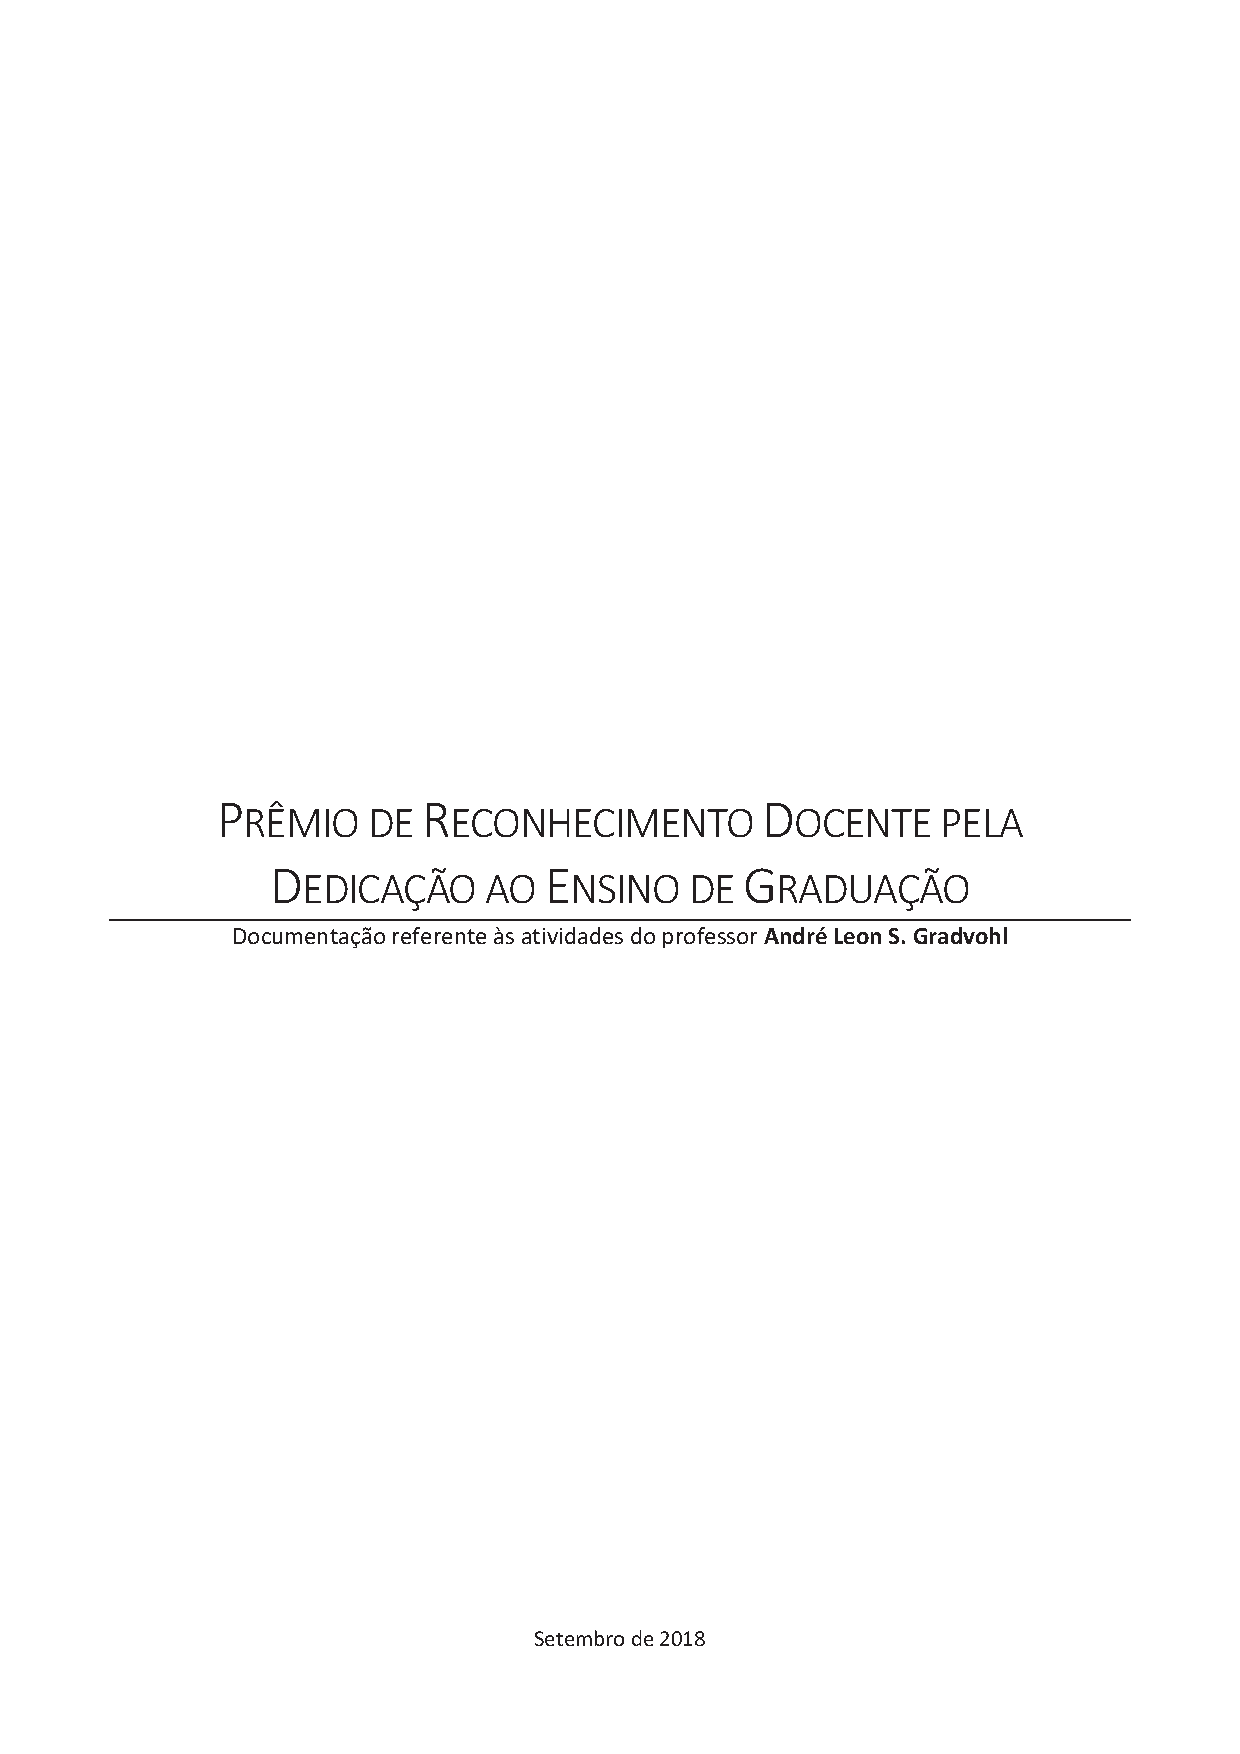
\includepdf[pages={1,{},2,{}}]{Capa_Preambulo}
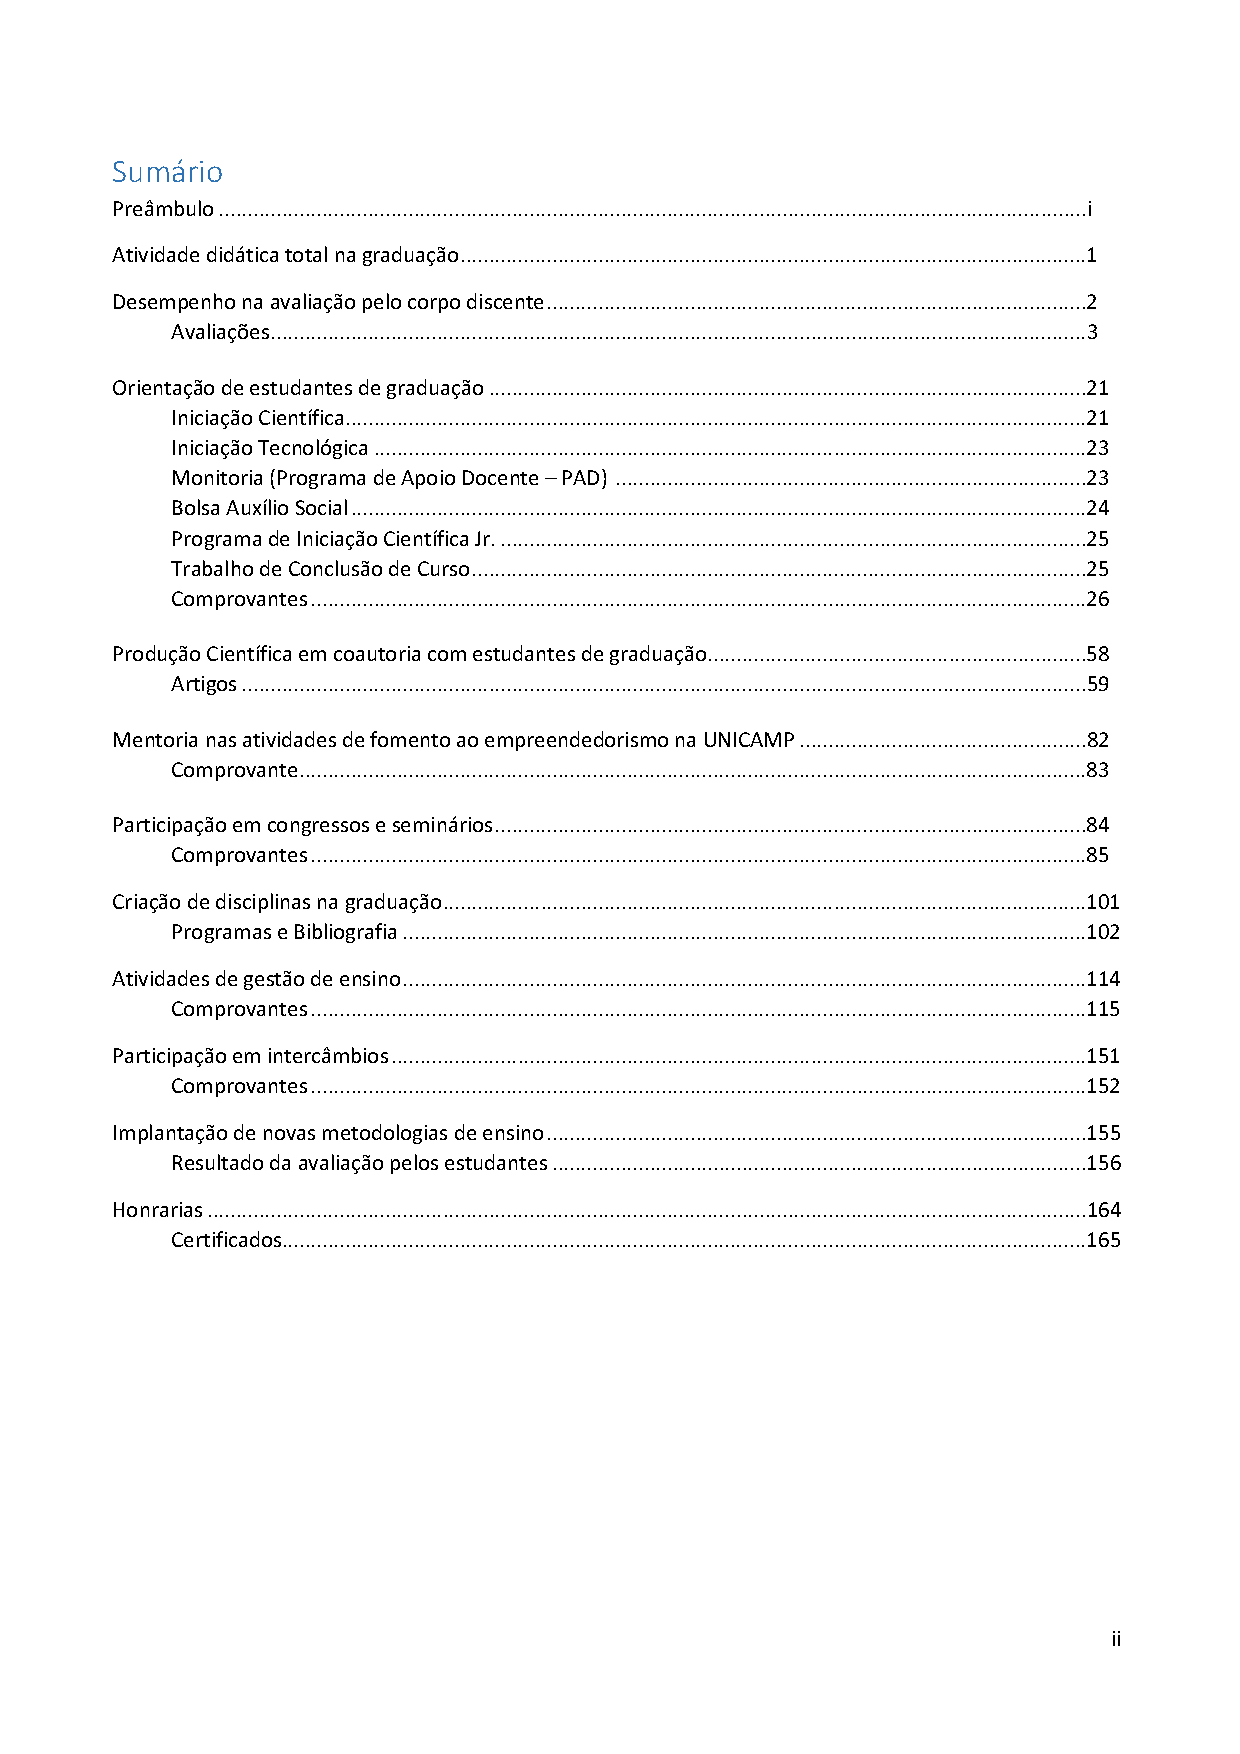
\includepdf[pages={1,{}}]{sumario}

%
%Resetando página para um
%
\setcounter{page}{1}
\includepdfset{pages=-,pagecommand=\thispagestyle{fancy}}
%
%
%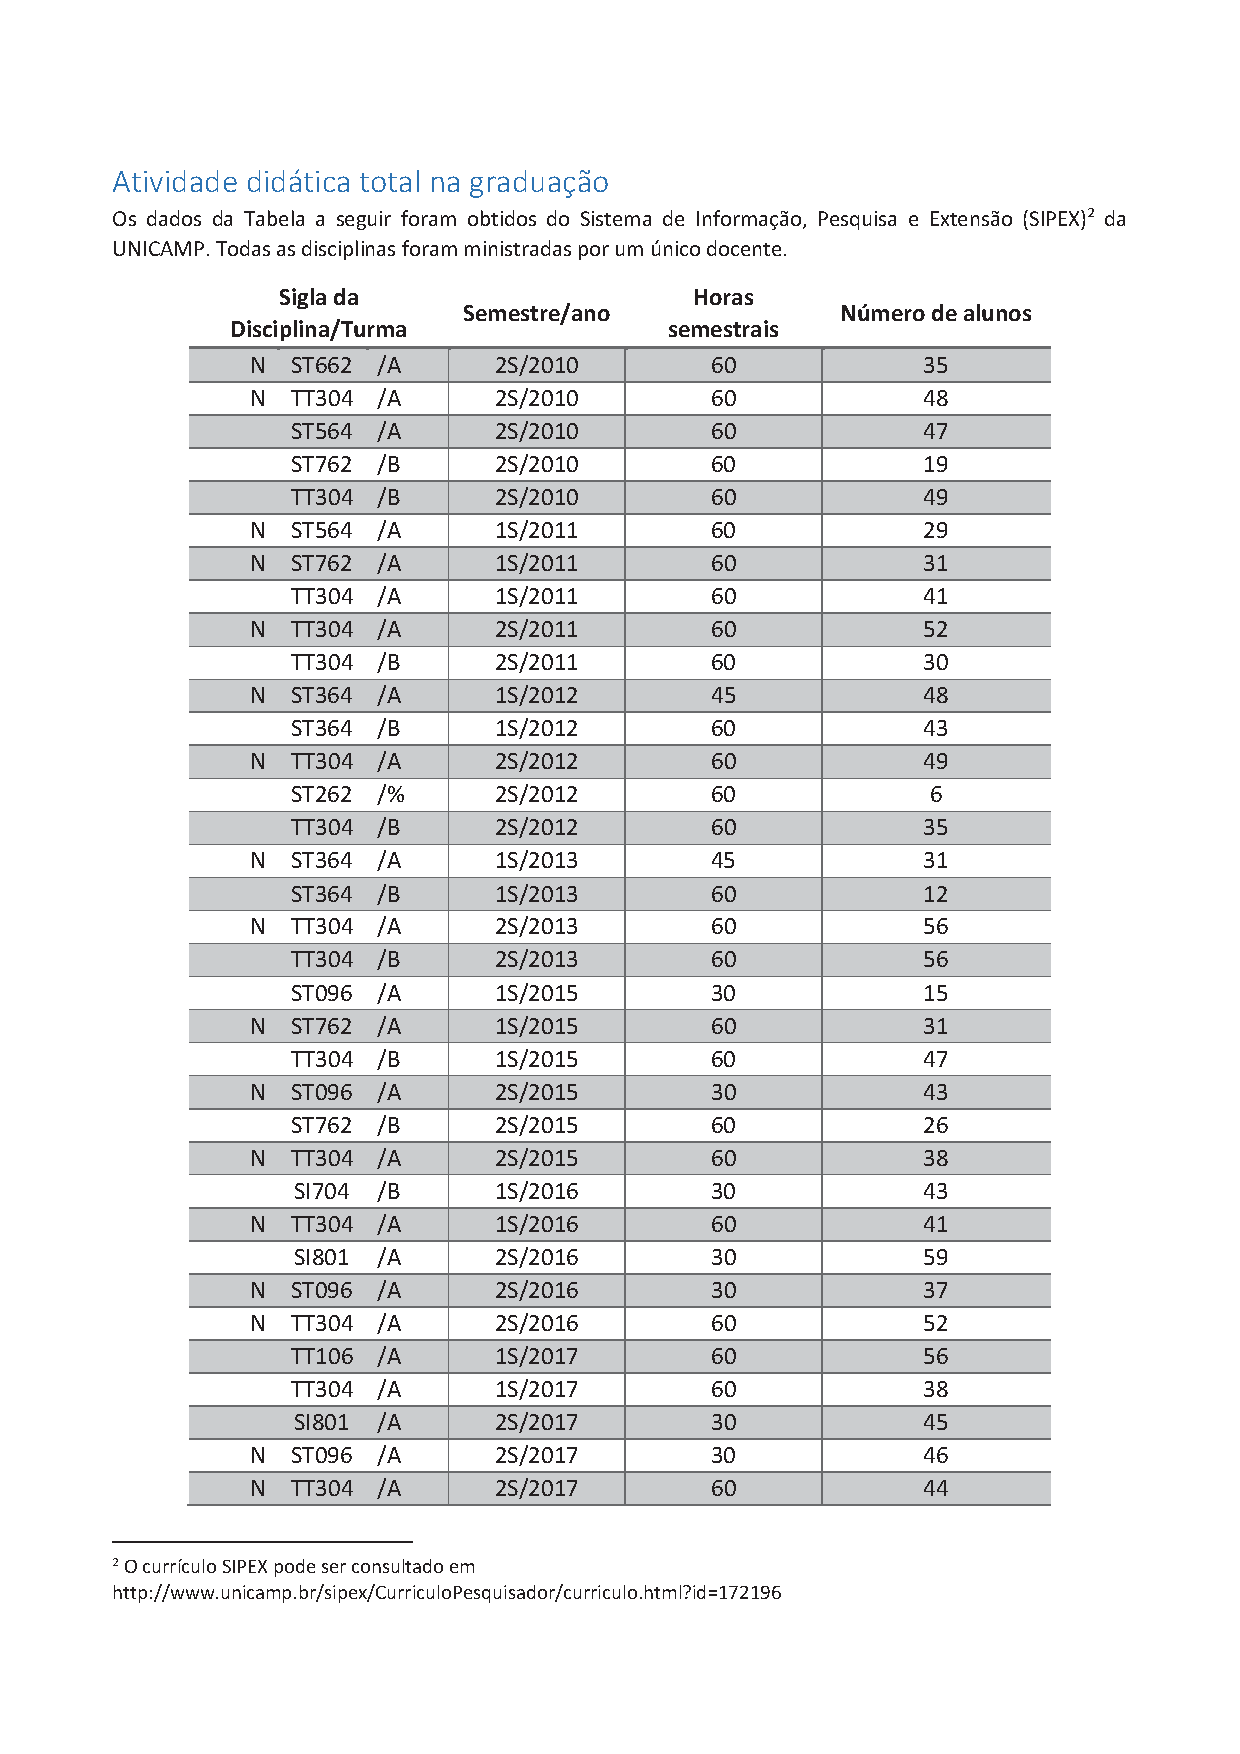
\includepdf{AtividadeDidatica}
%\includepdf{./docs/1_1_RelatorioPAG}
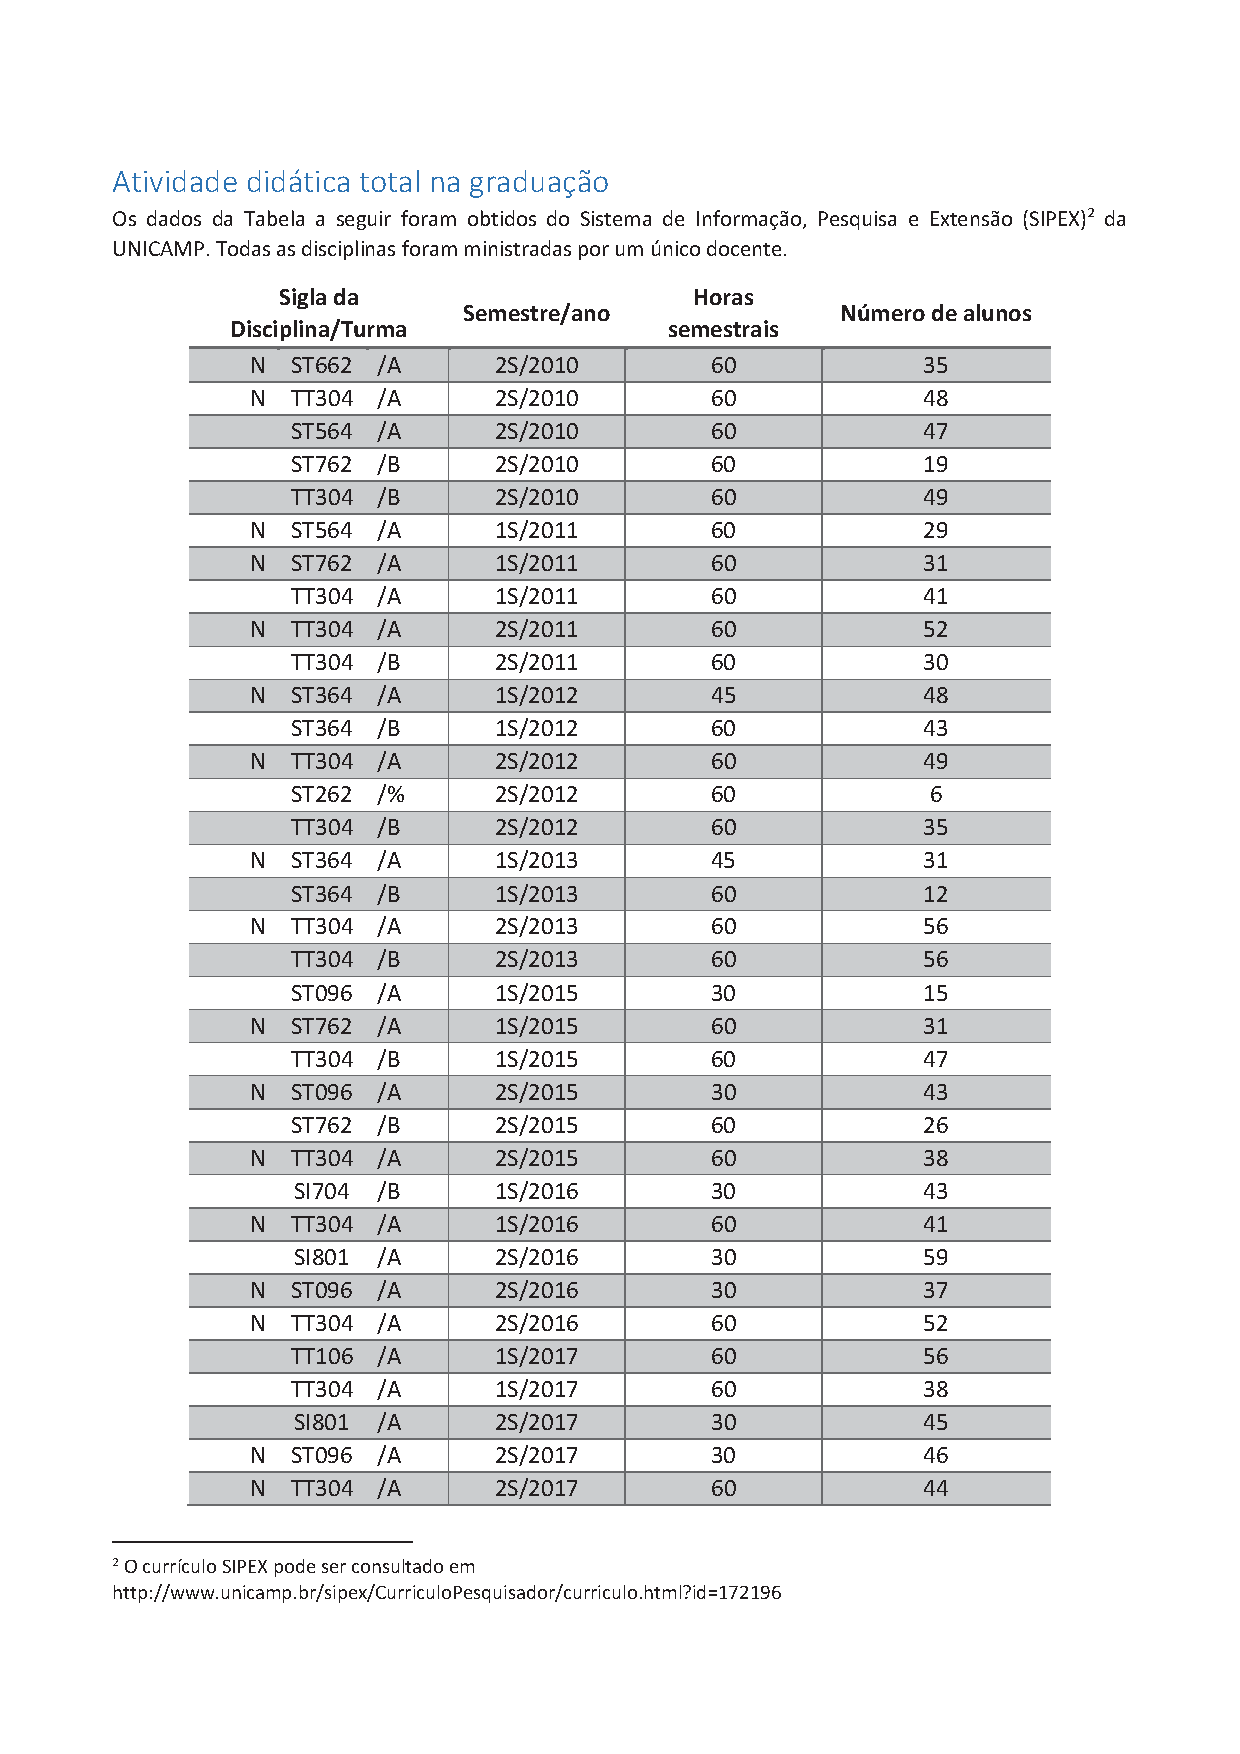
\includepdf{AtividadeDidatica}
\includepdf{./docs/1_1_RelatorioPAG}
%
%
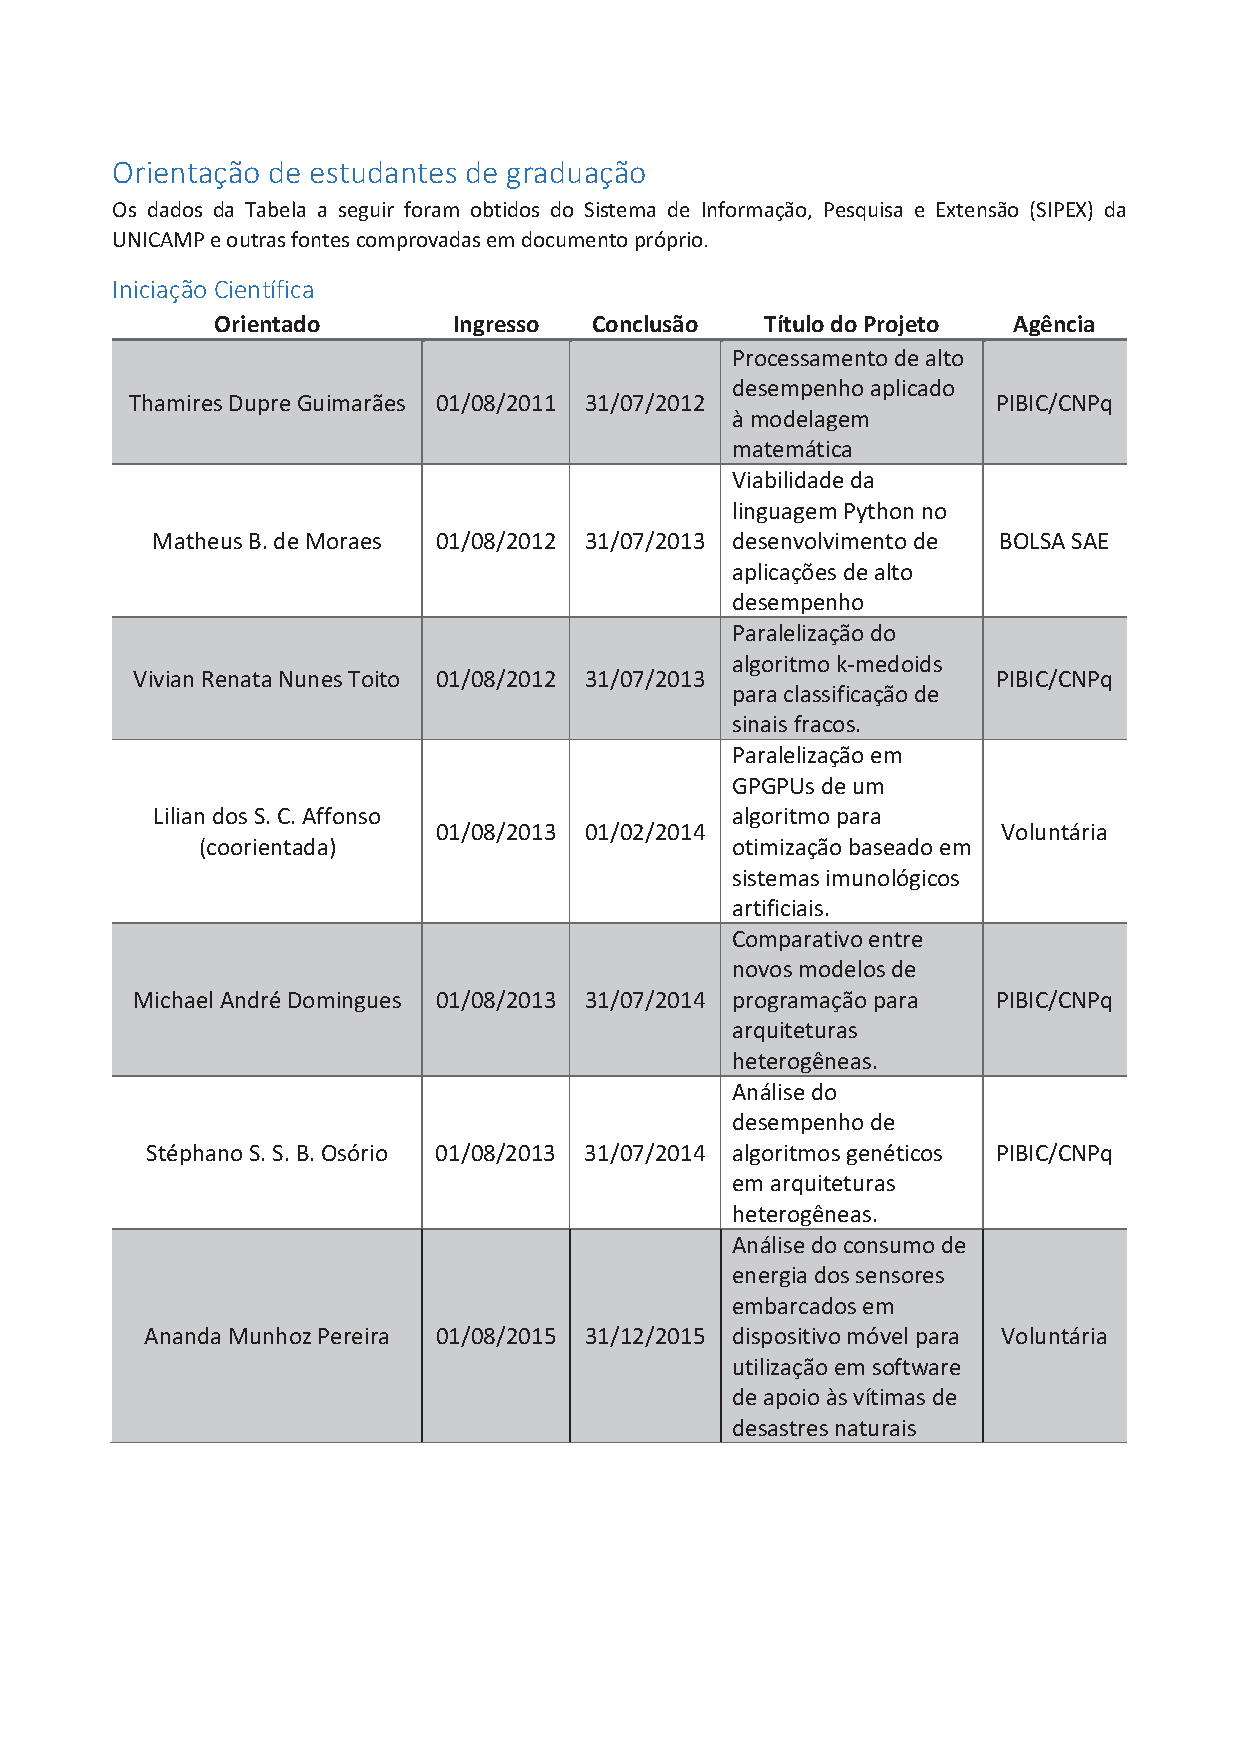
\includepdf{OrientacaoAlunos}
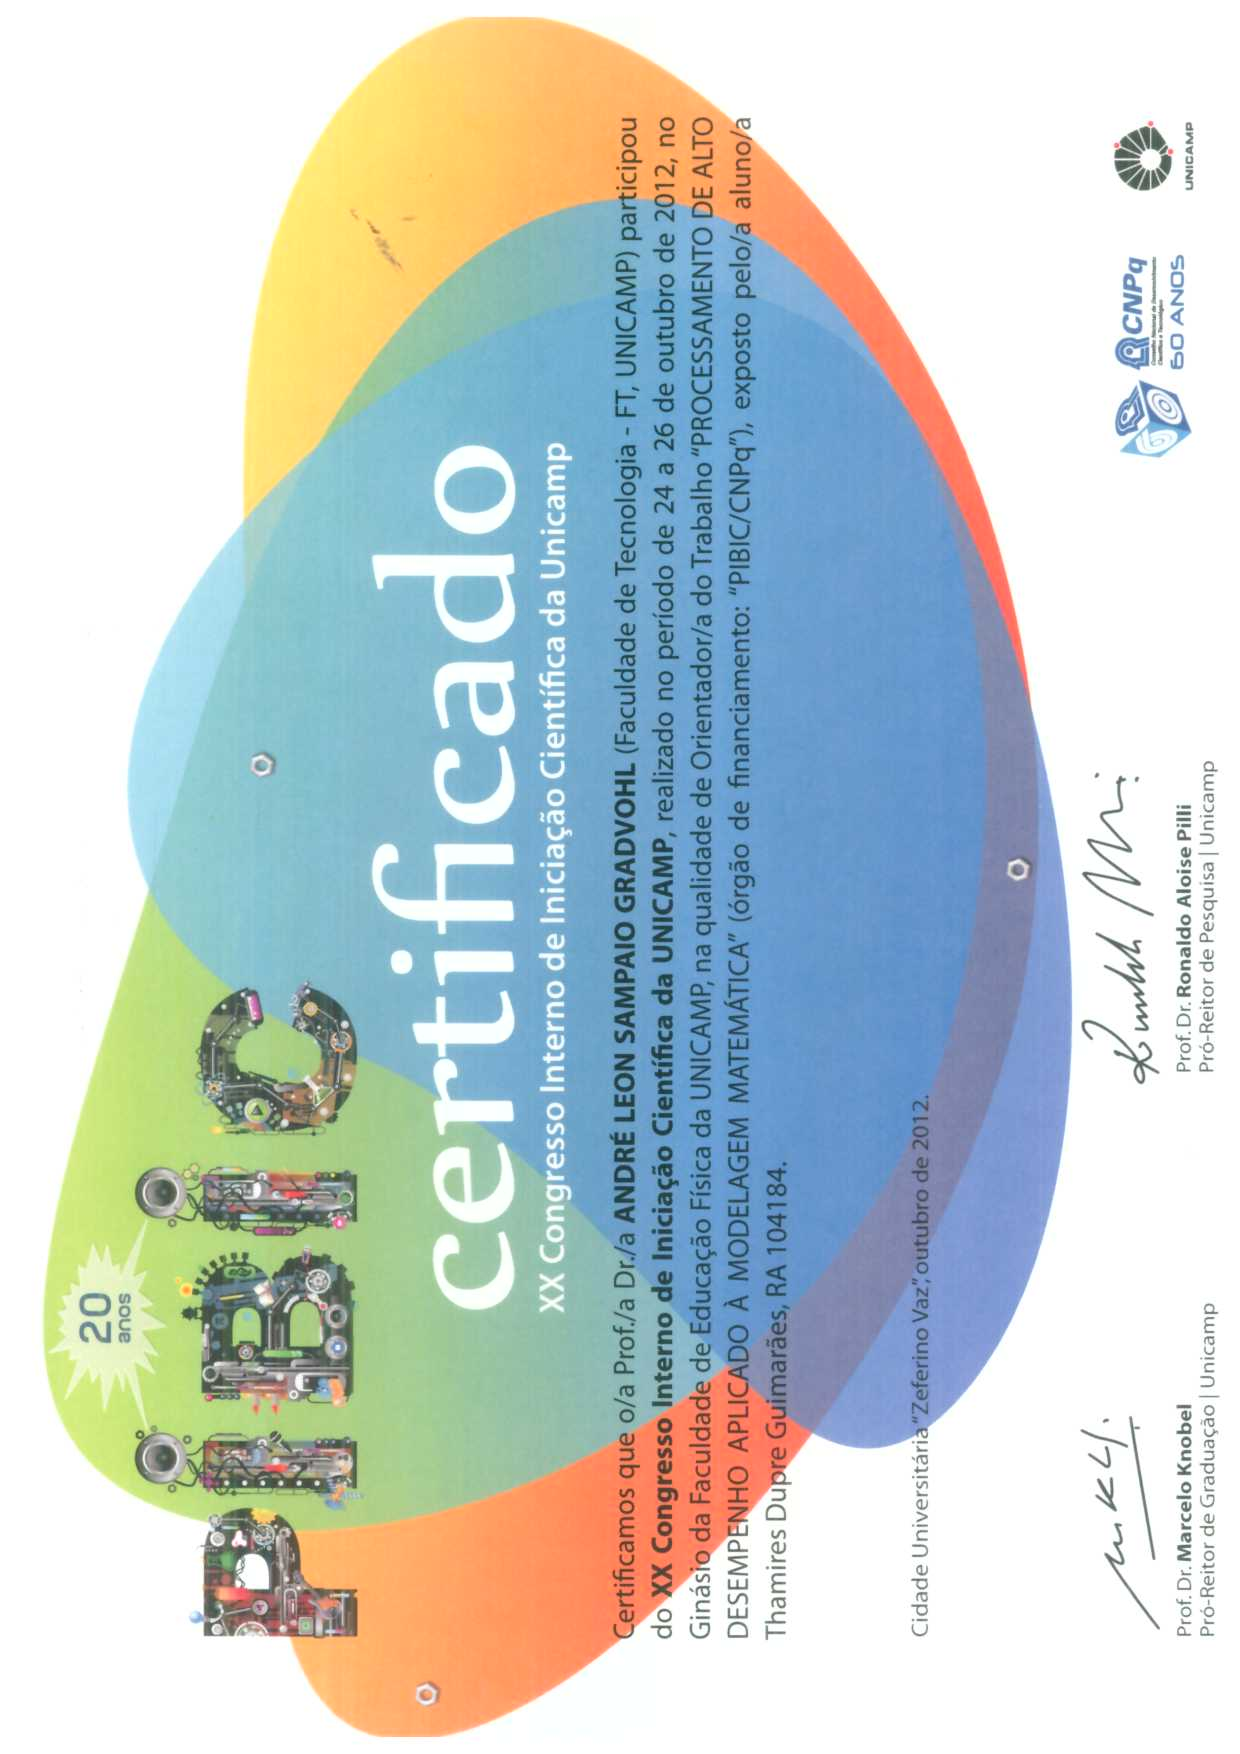
\includepdf{./docs/CertificadosPIBIC2012_2017}
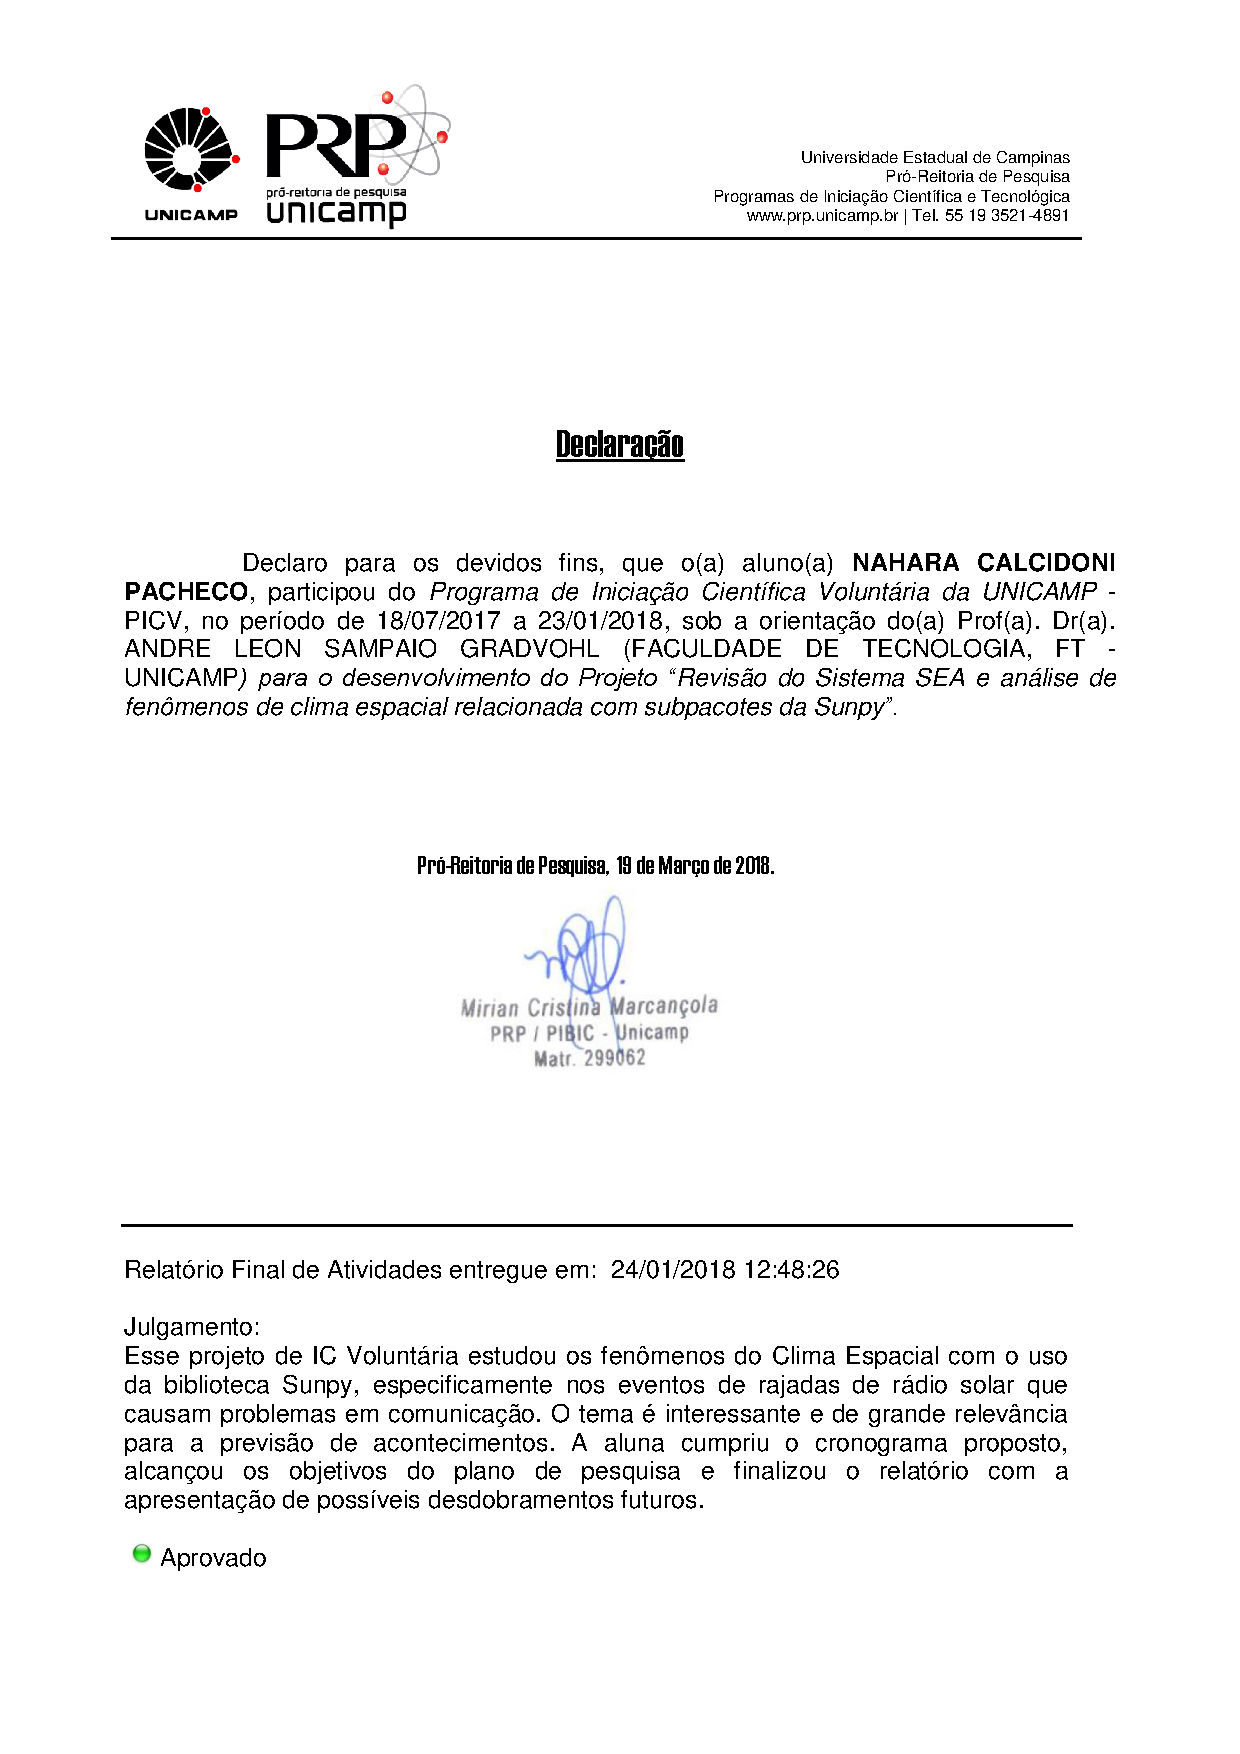
\includepdf{./docs/CertificadoCV2017_NaharaPacheco}
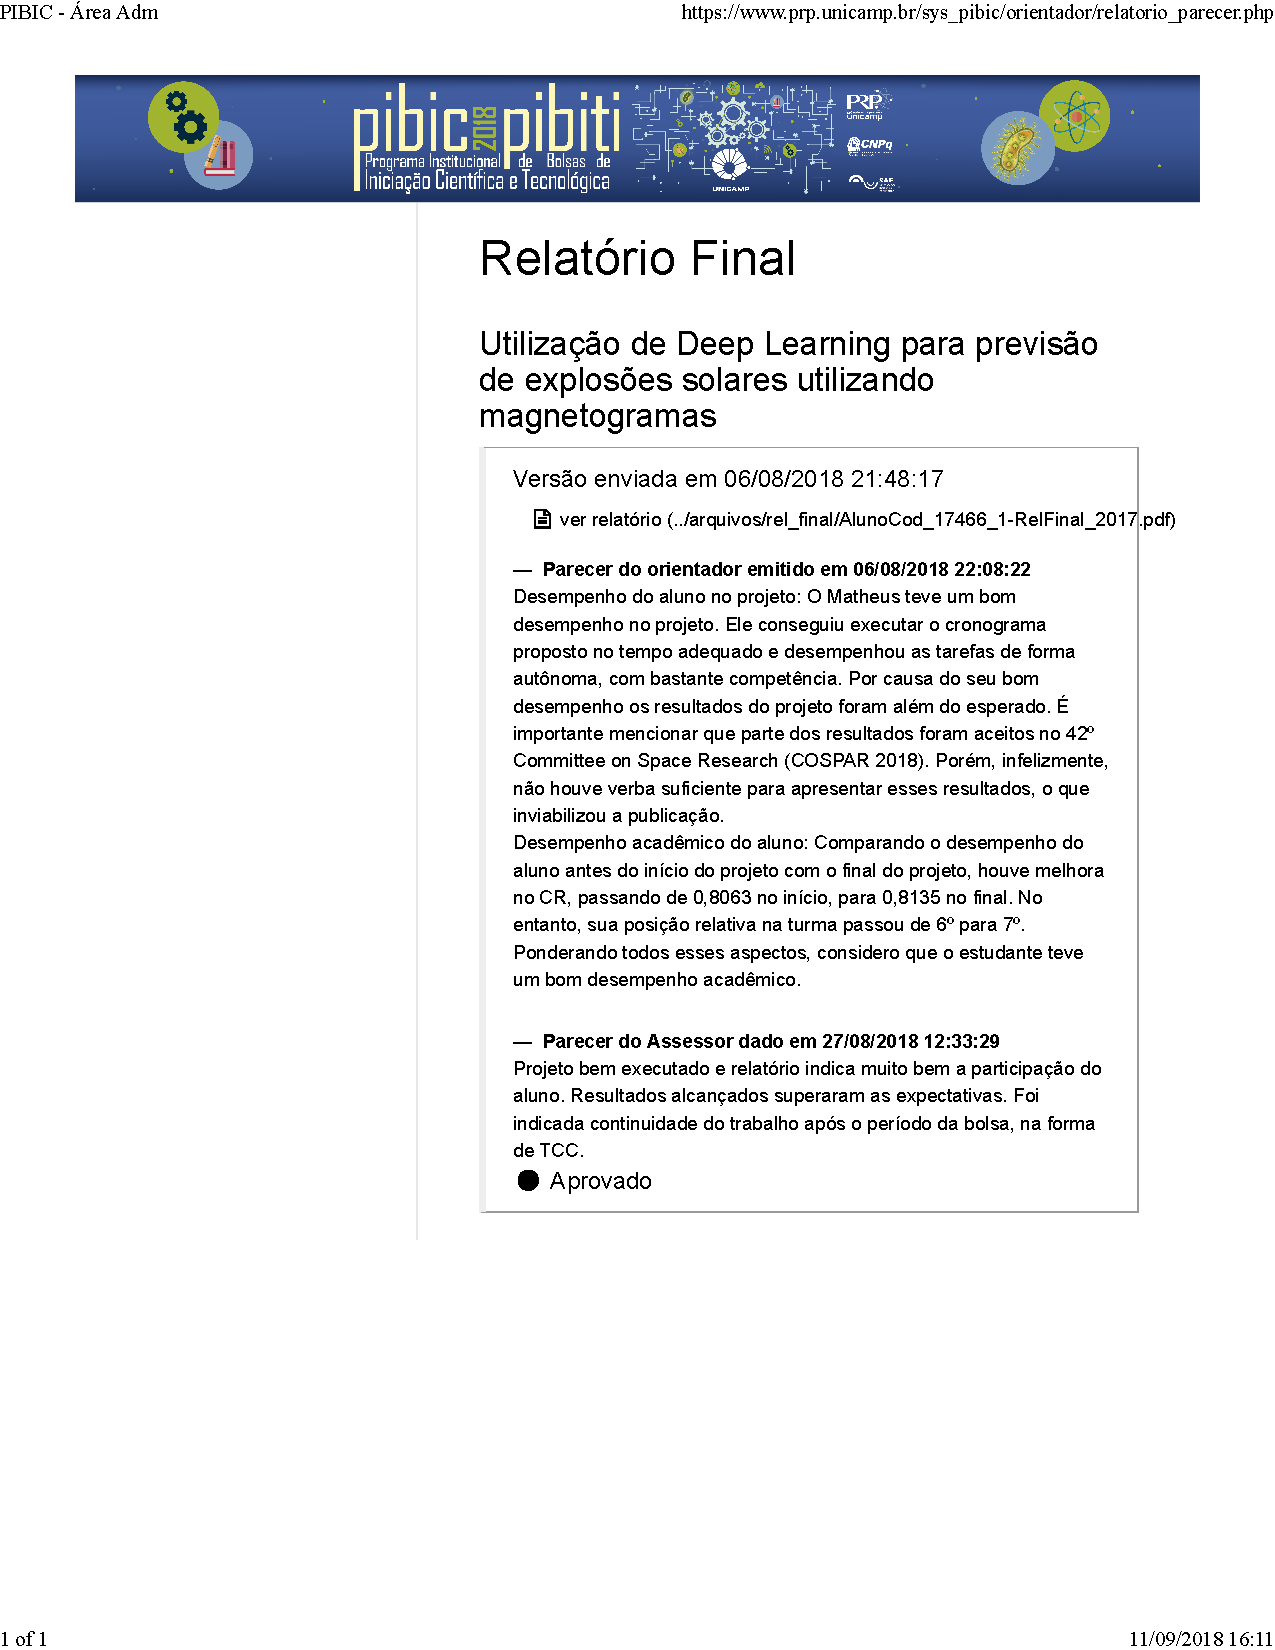
\includepdf{./docs/AprovacaoIC_MatheusEvers}
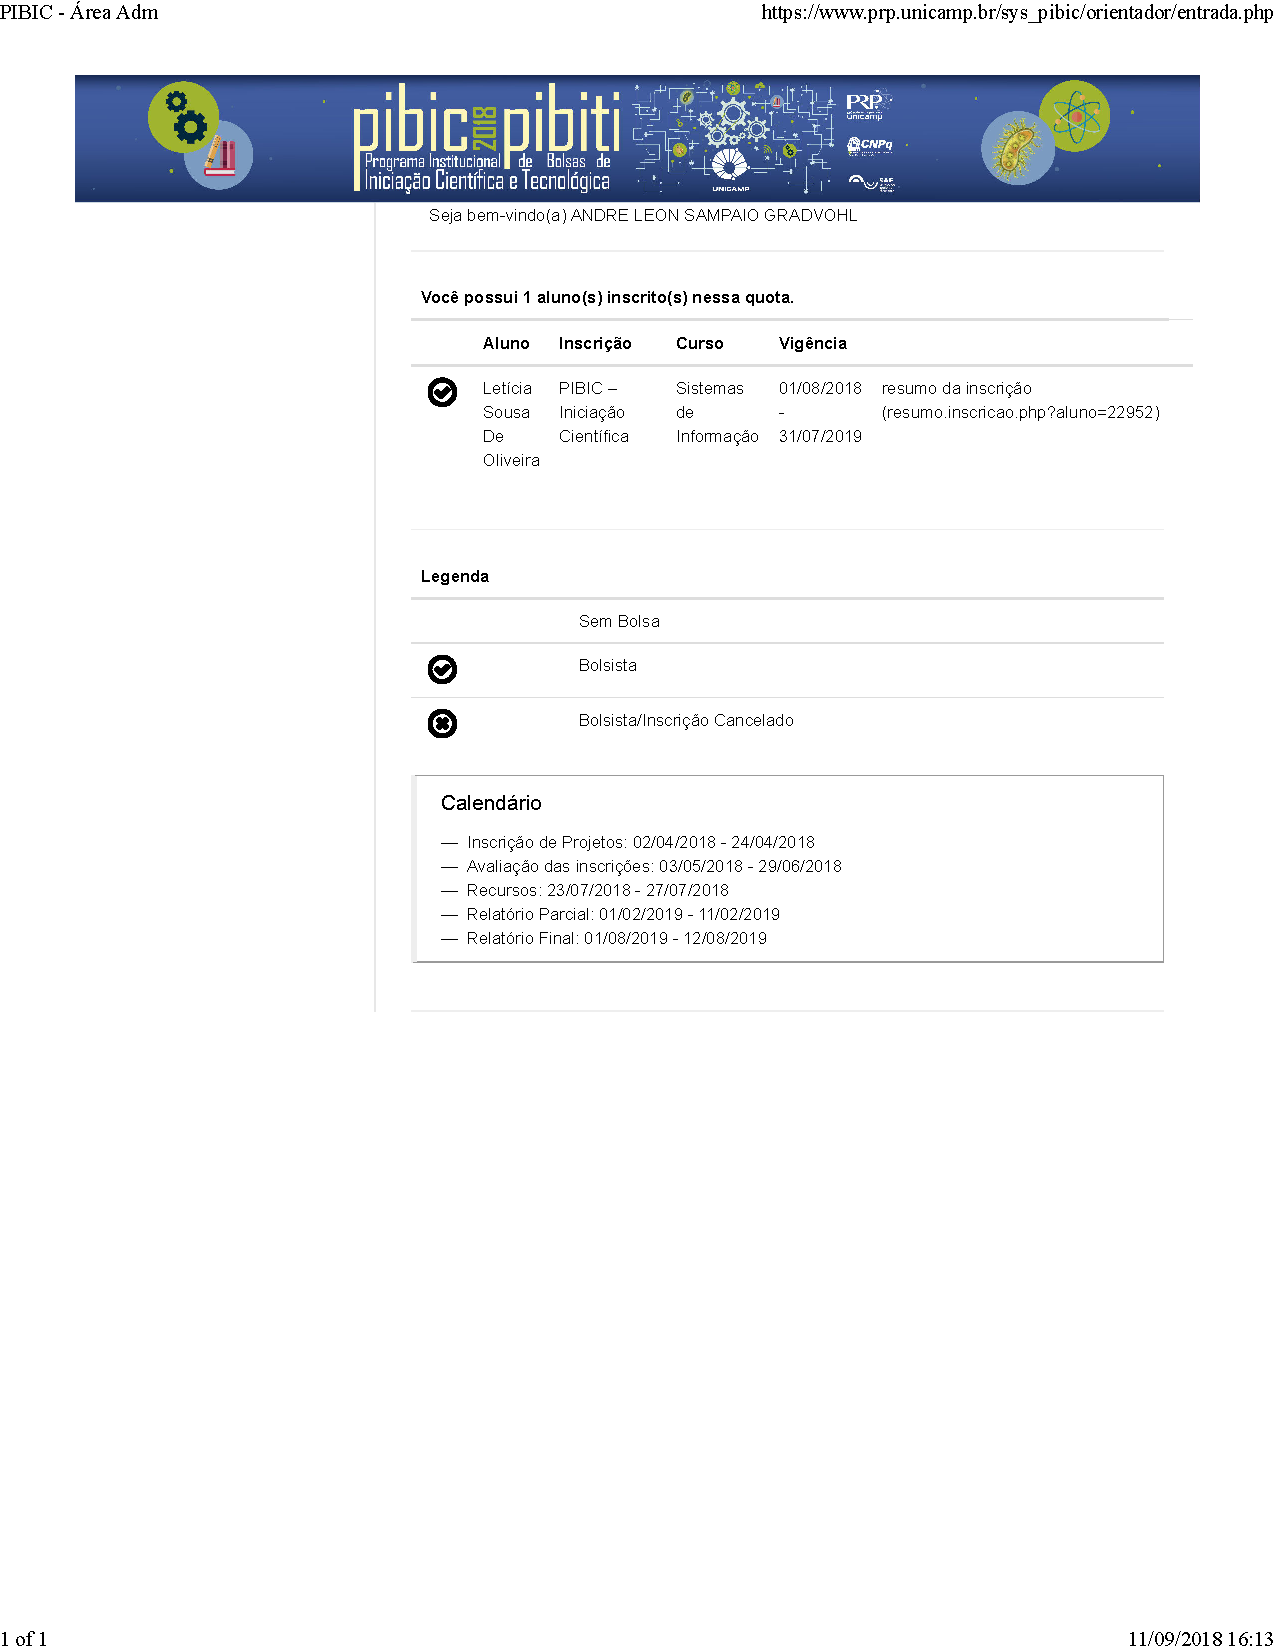
\includepdf{./docs/AprovacaoIC_LeticiaOliveira}
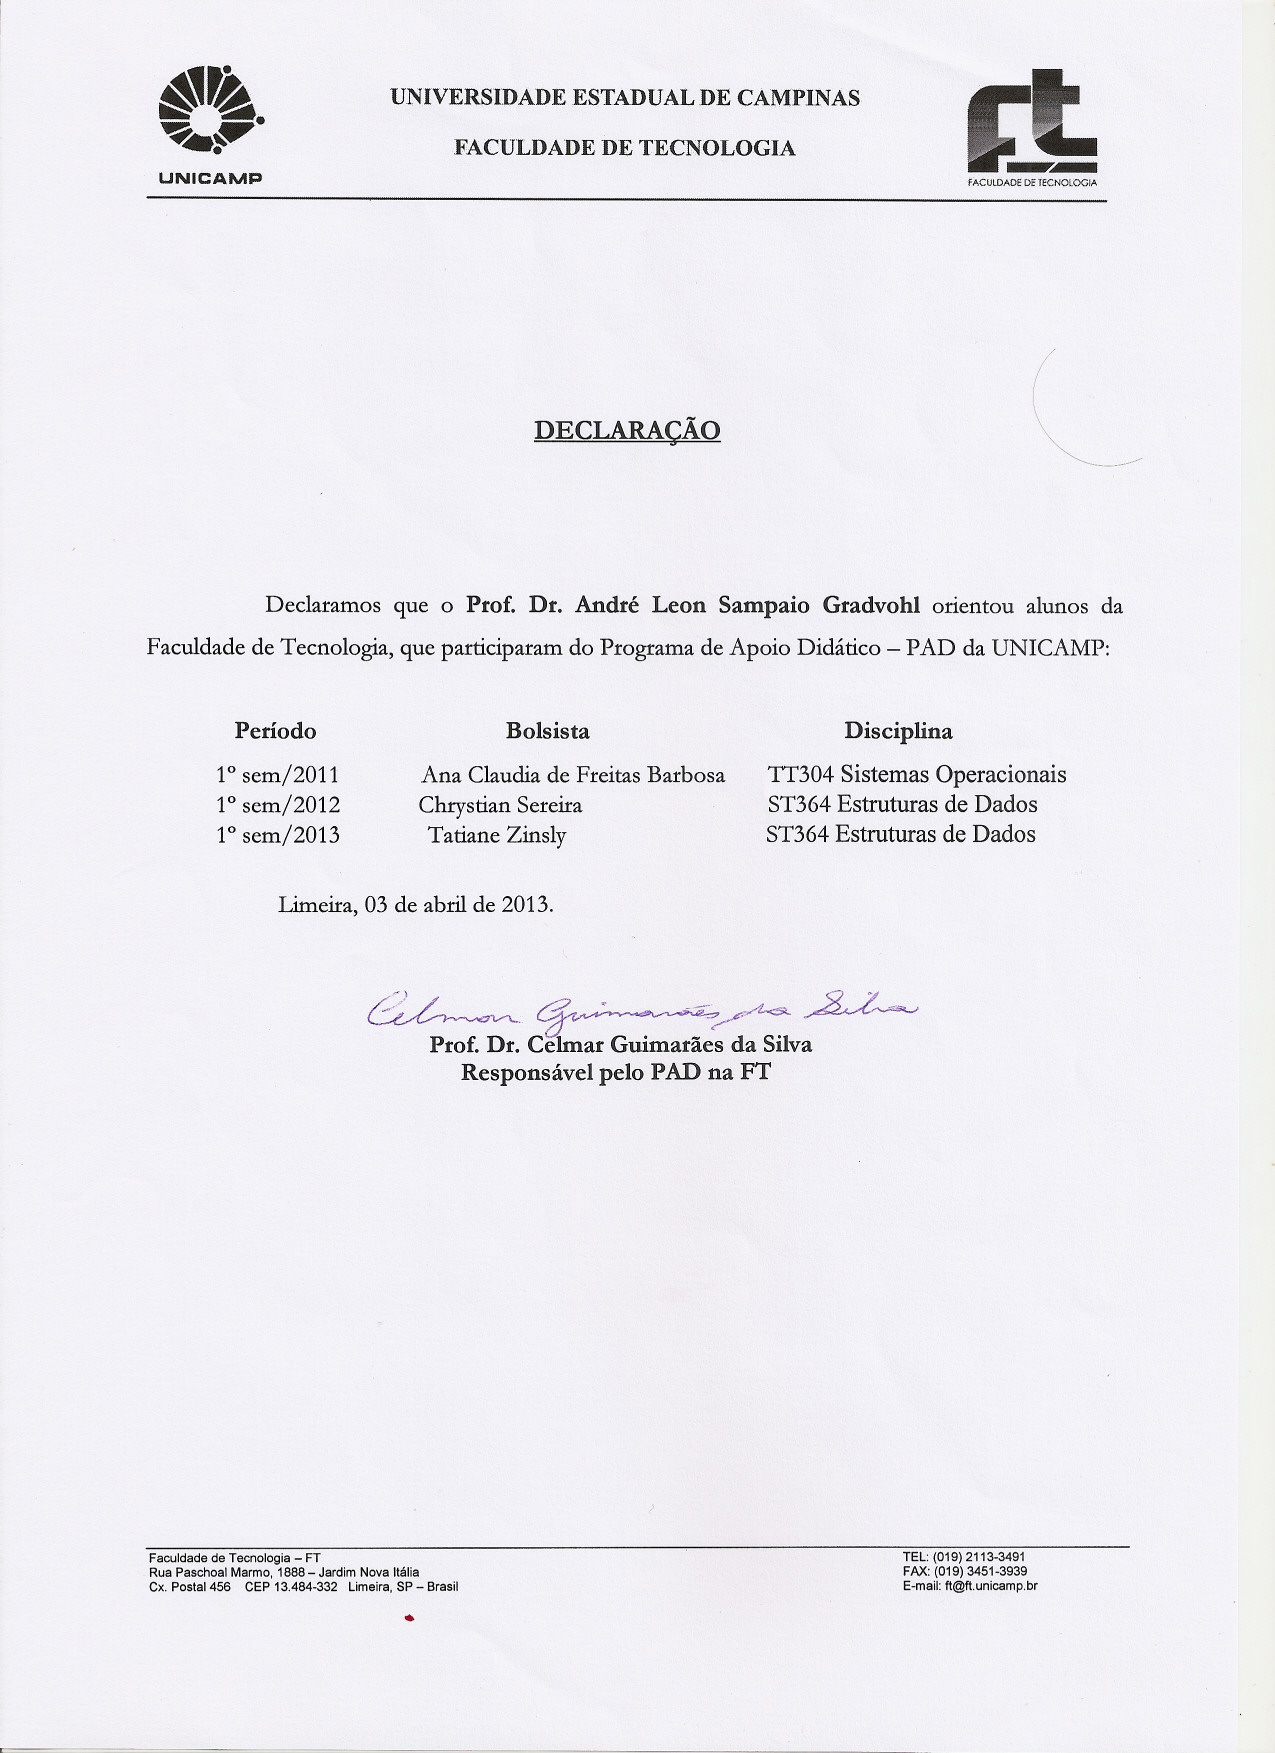
\includepdf{./docs/2_6_CertificadosOrientacaoPAD_2013_2017}
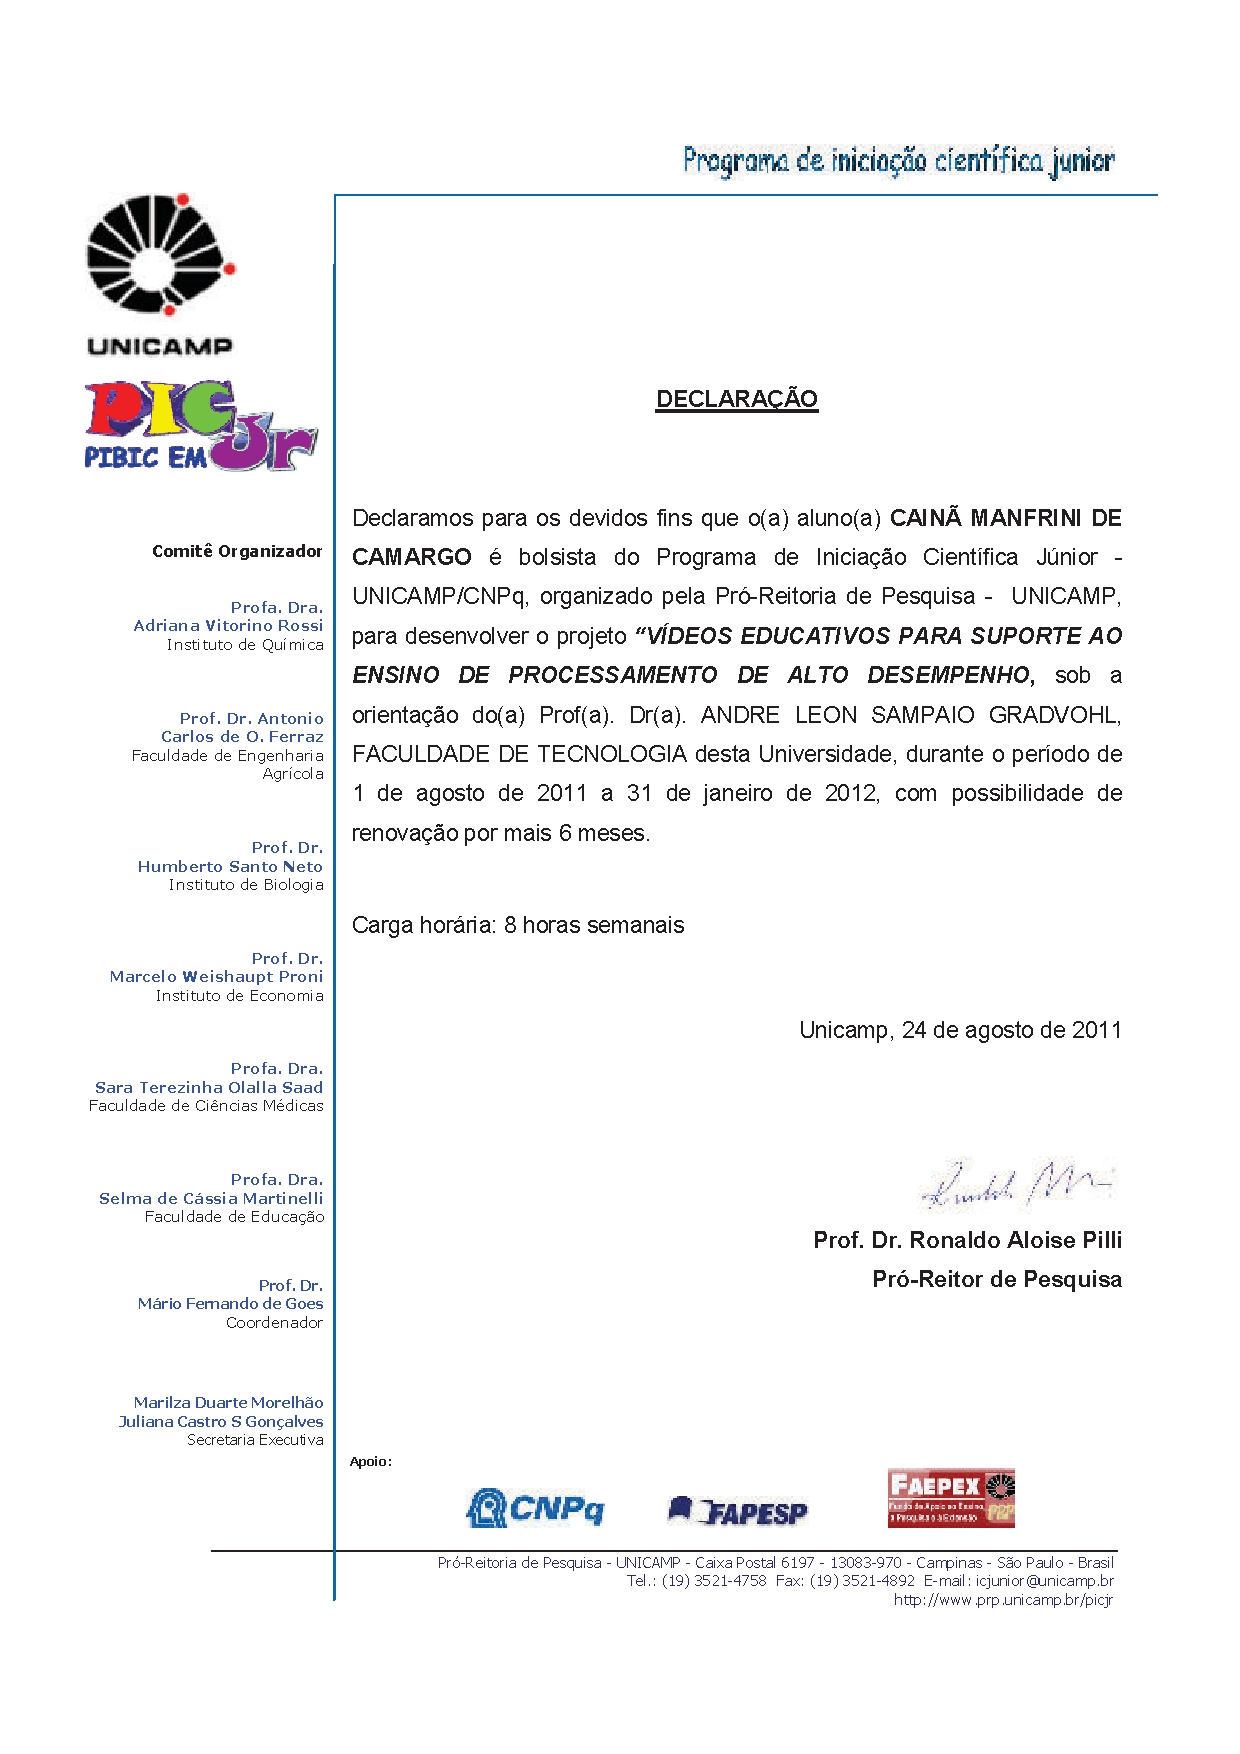
\includepdf{./docs/2_7_declaracaoPicJR}
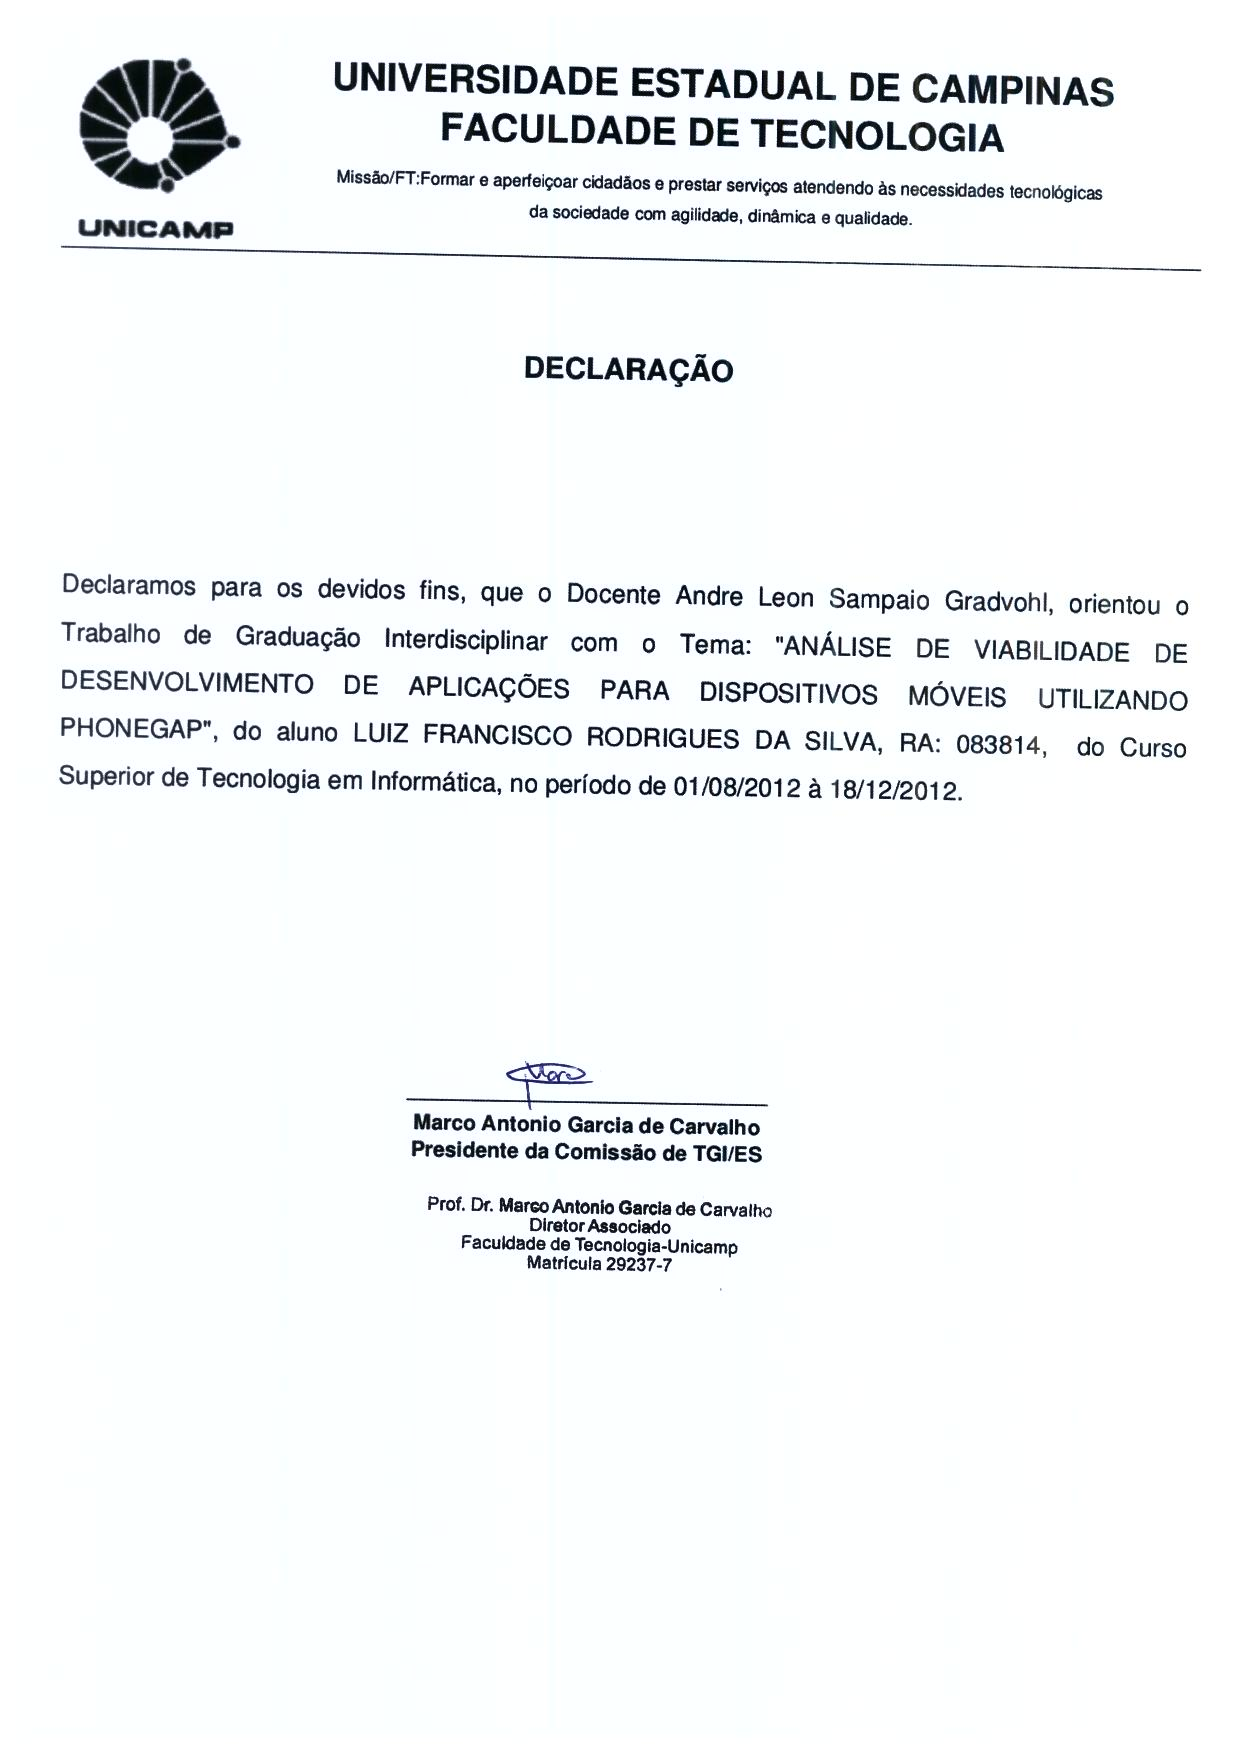
\includepdf{./docs/2_8_declaracaoTCC_2012_2010}
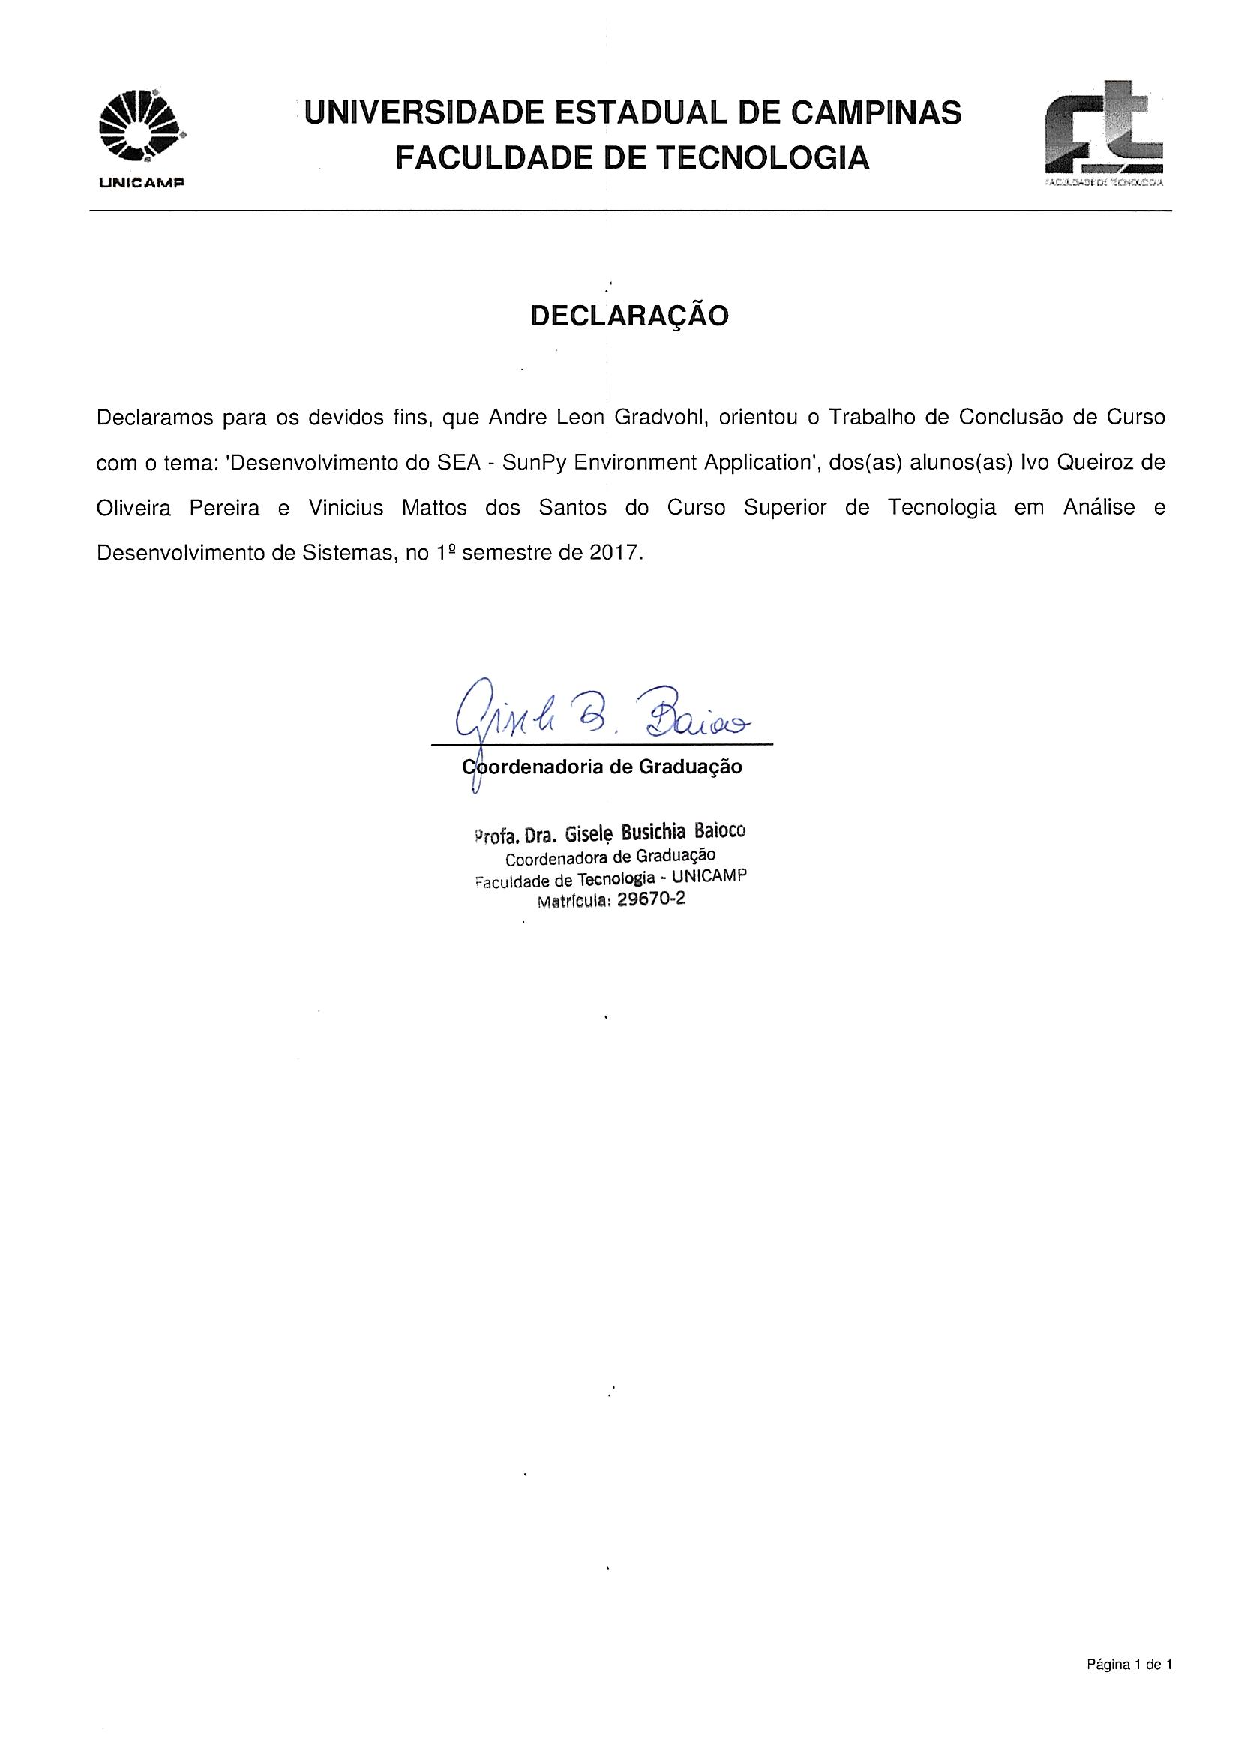
\includepdf{./docs/2_8_declaracaoTCC_2012_2017}
%
%
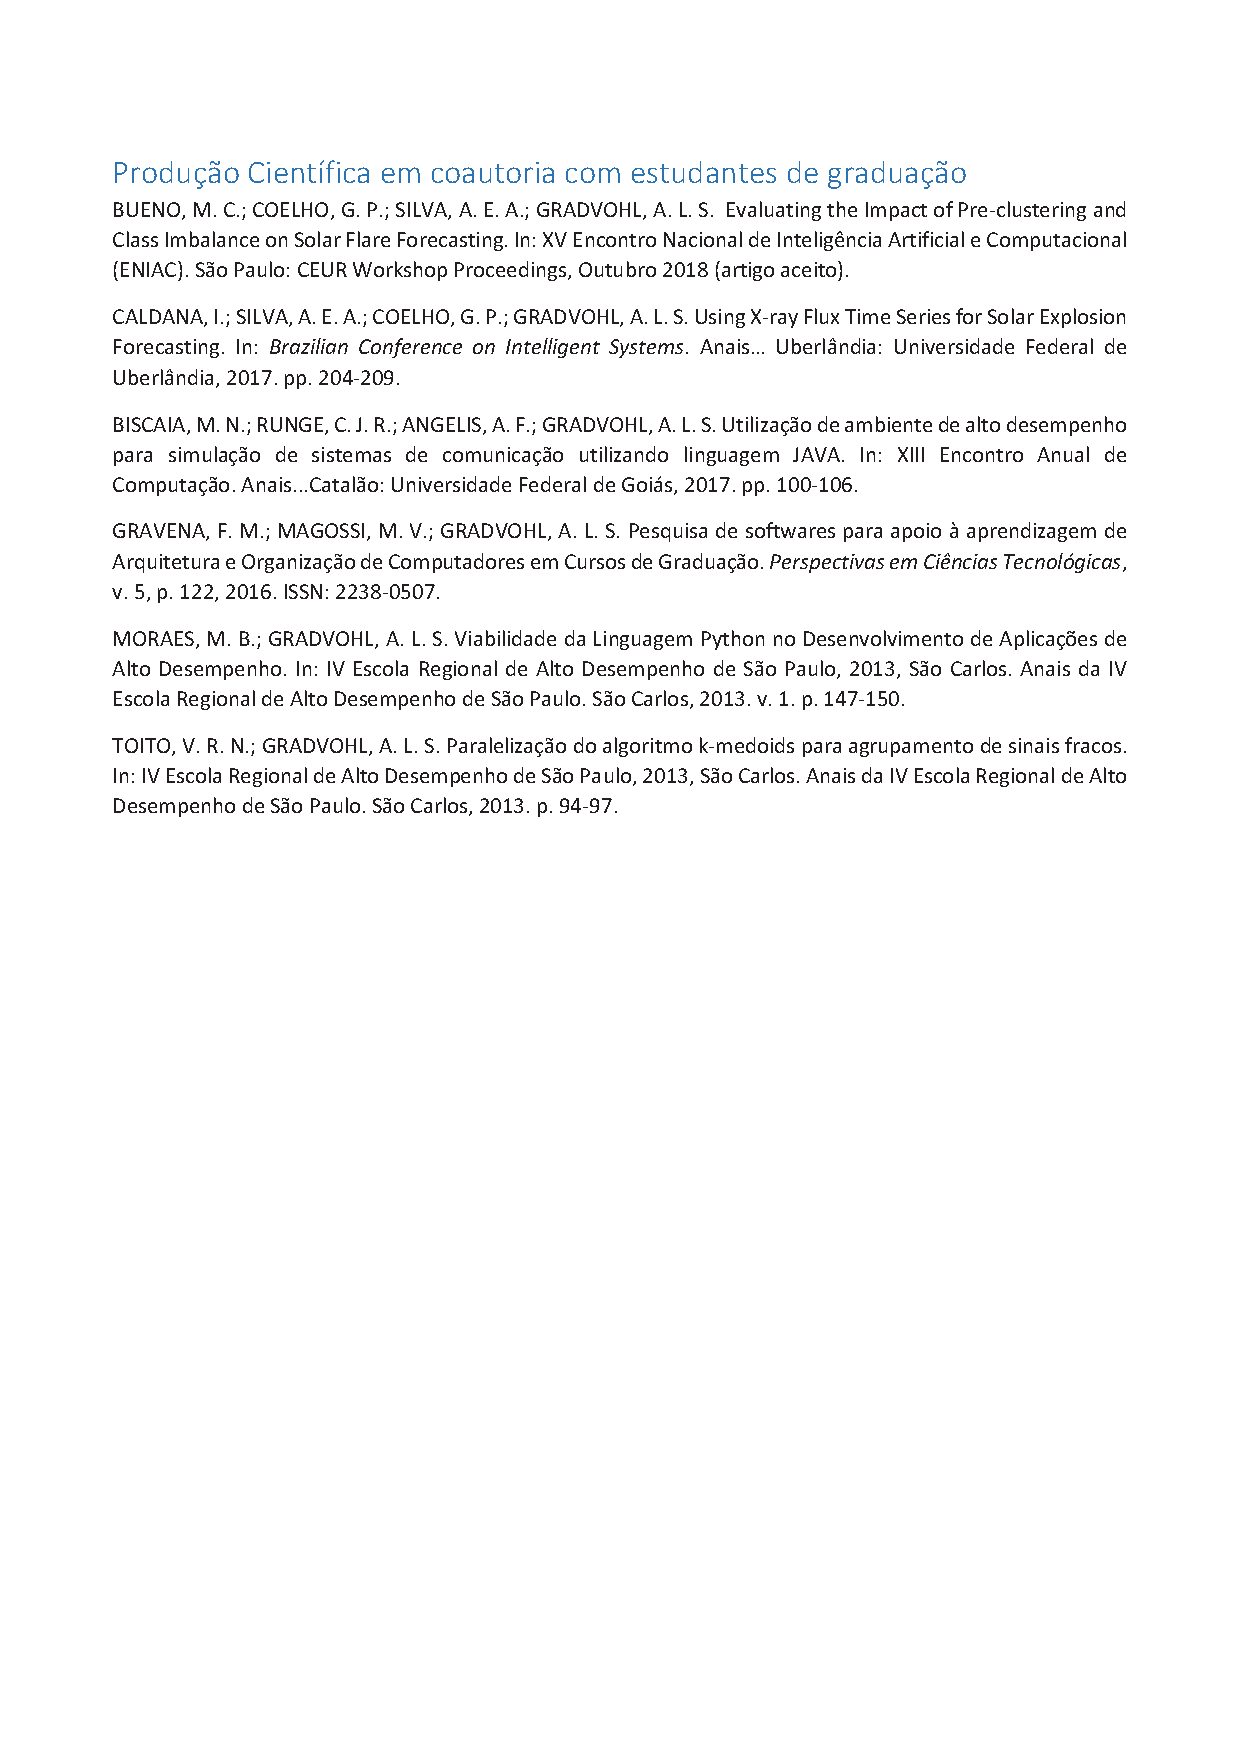
\includepdf{ProducaoCientifica.pdf}
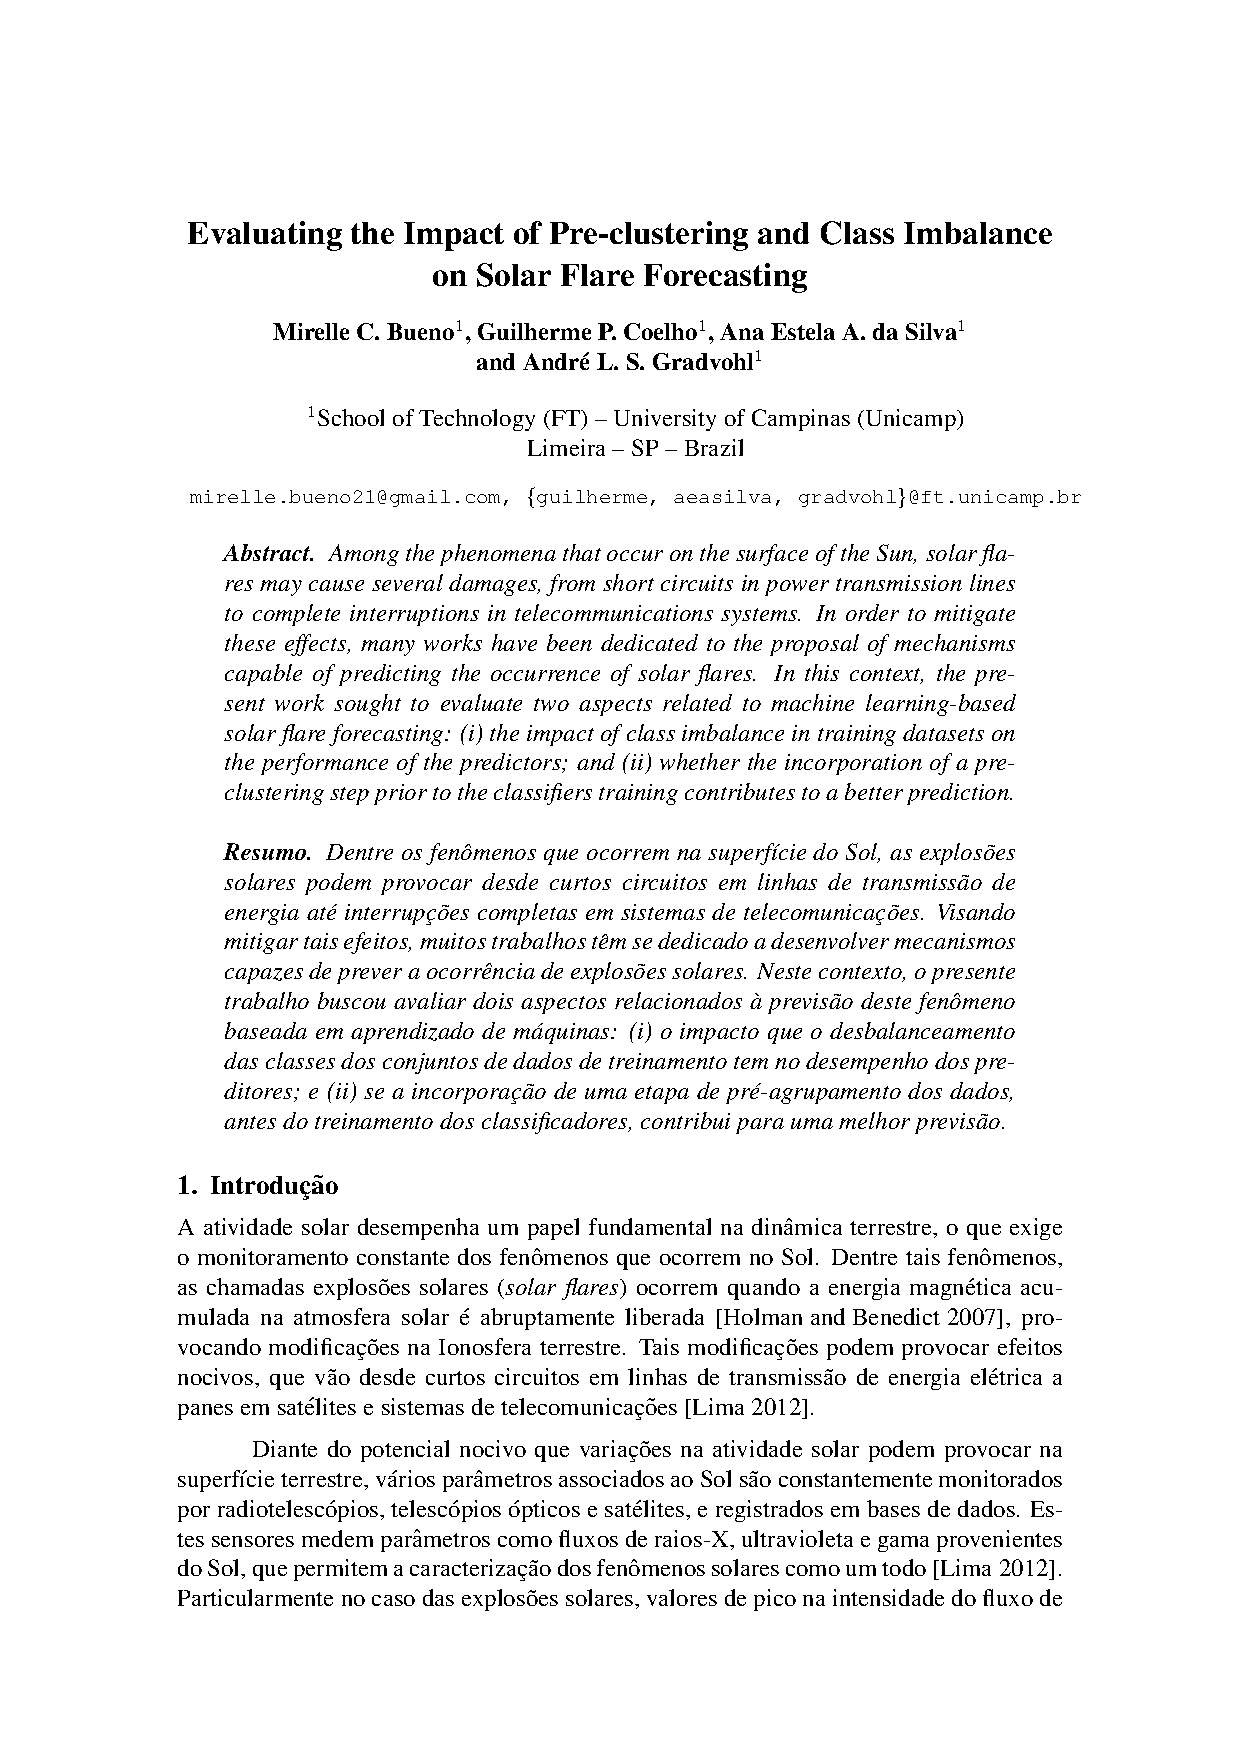
\includepdf[nup=1x2,frame,landscape=true, width=118mm, height=195mm]{./docs/ArtigoMirelle_2018}
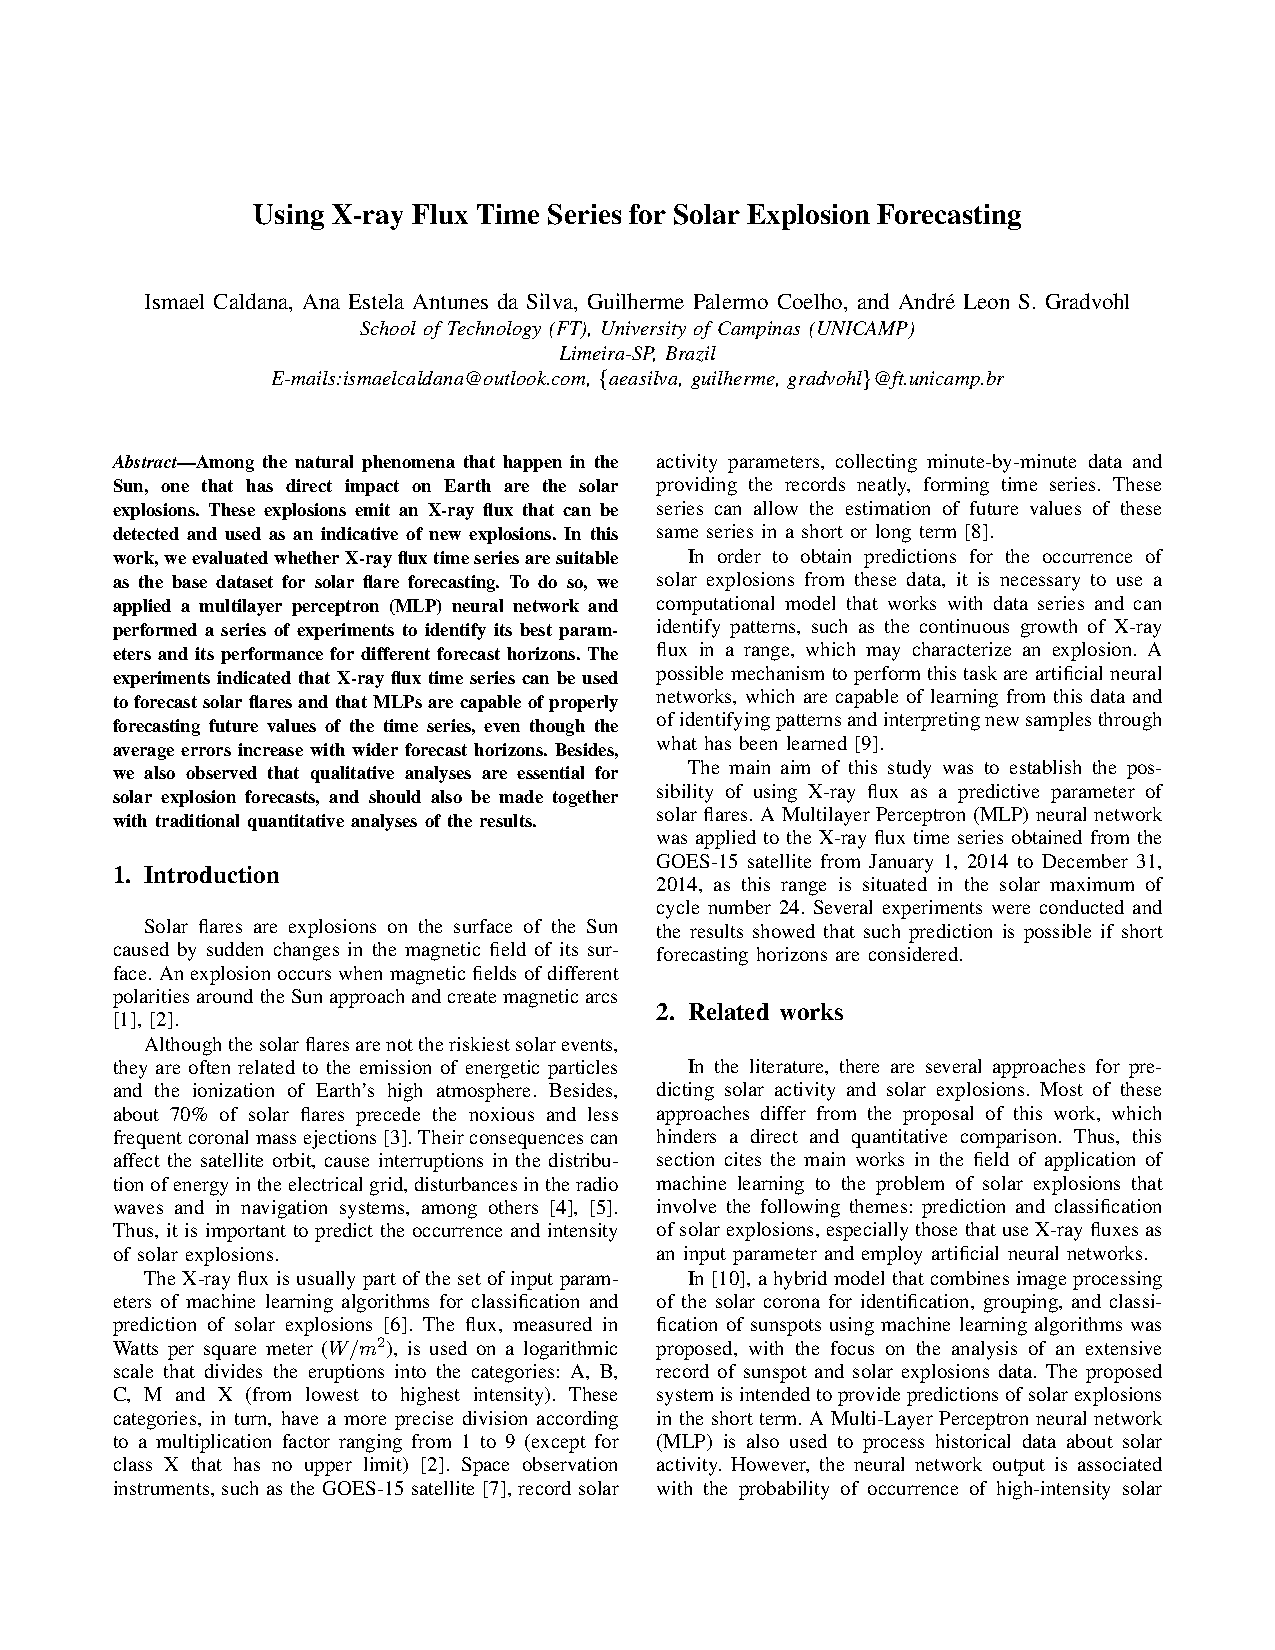
\includepdf[nup=1x2,frame,landscape=true,  width=118mm, height=195mm]{./docs/3_1_ArtigoUsingX-Ray-Flux}
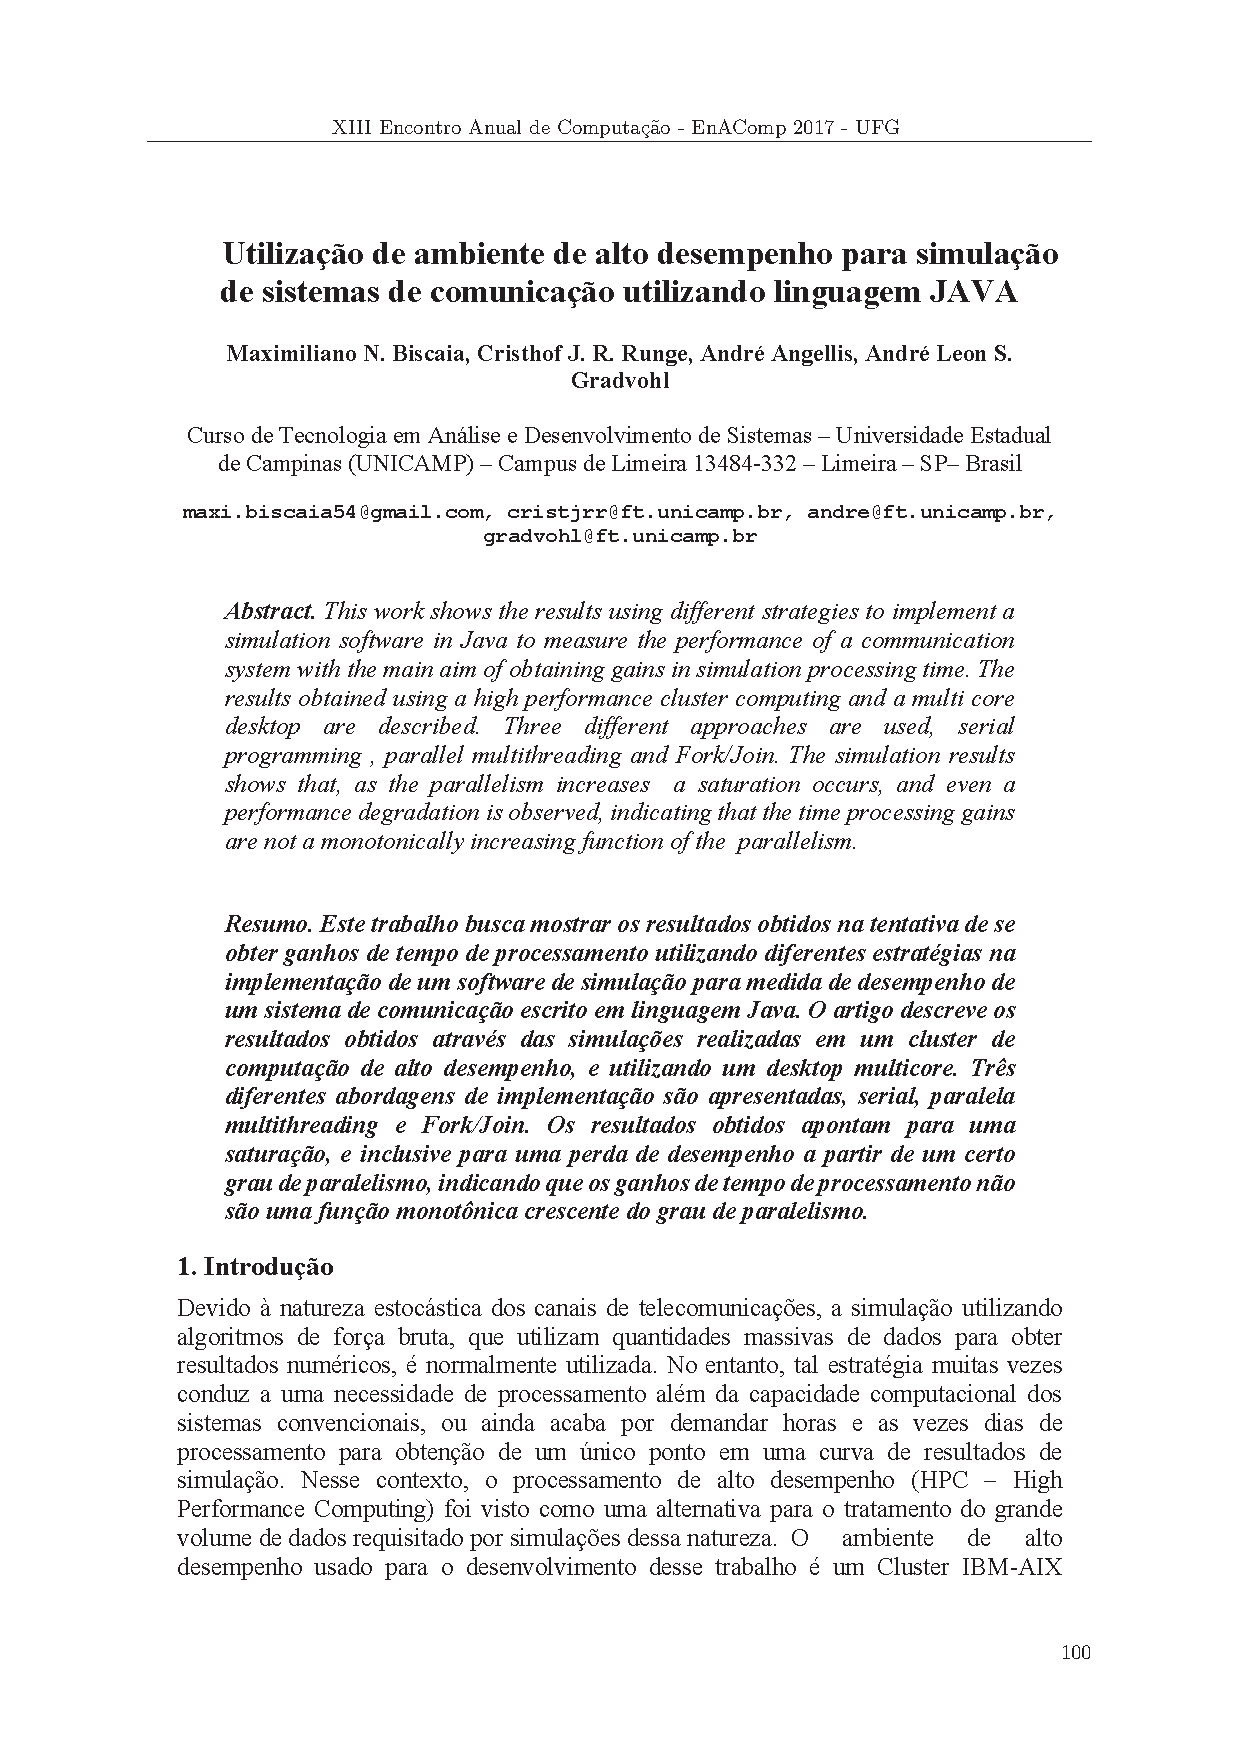
\includepdf[nup=1x2,frame,landscape=true,  width=118mm, height=195mm]{./docs/3_2_Resumo_UtilizacaoAmbienteAltoDesempenhoJava_Enacomp2017}
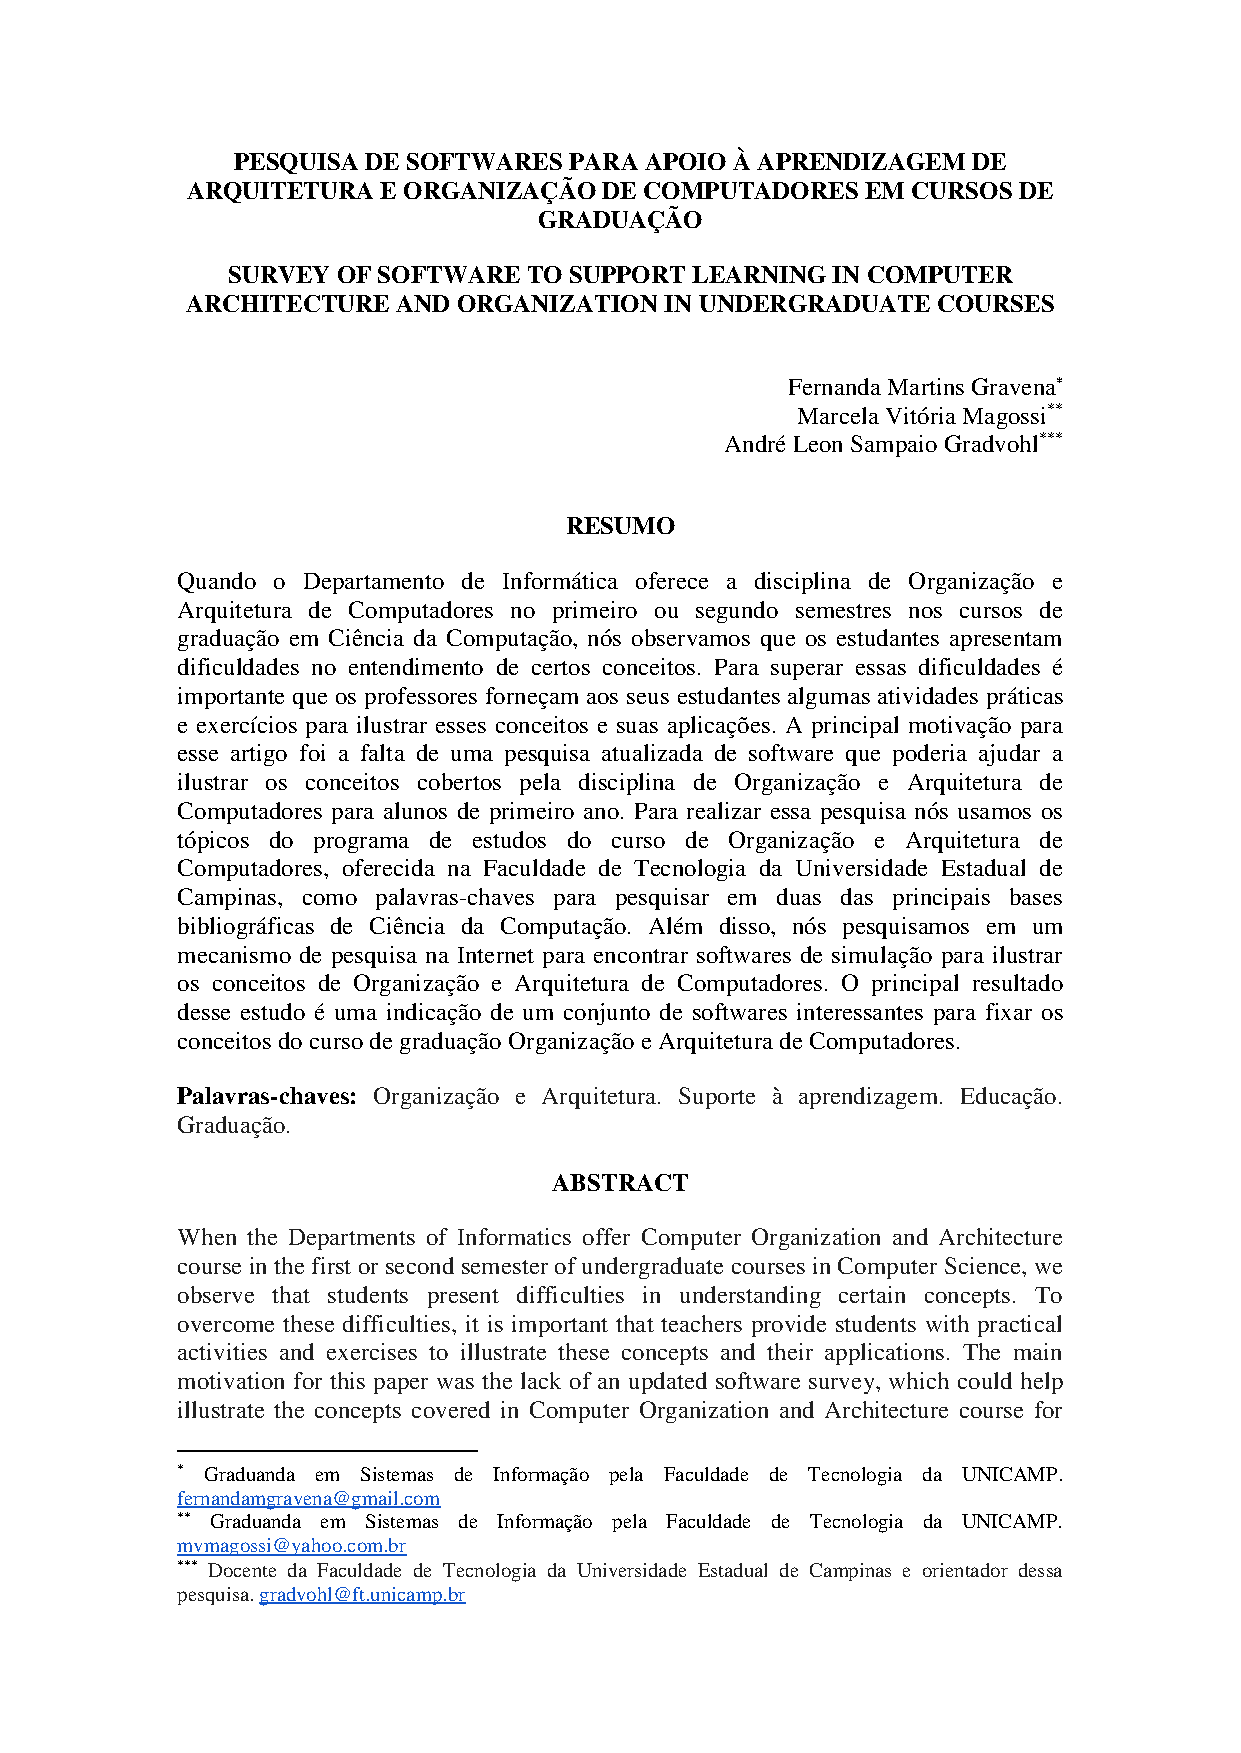
\includepdf[nup=1x2,frame,landscape=true,  width=118mm, height=195mm]{./docs/3_3_ArtigoPesquisasSoftwareApoioAprendizagemArquiteturaOrganizacaoComputadores}
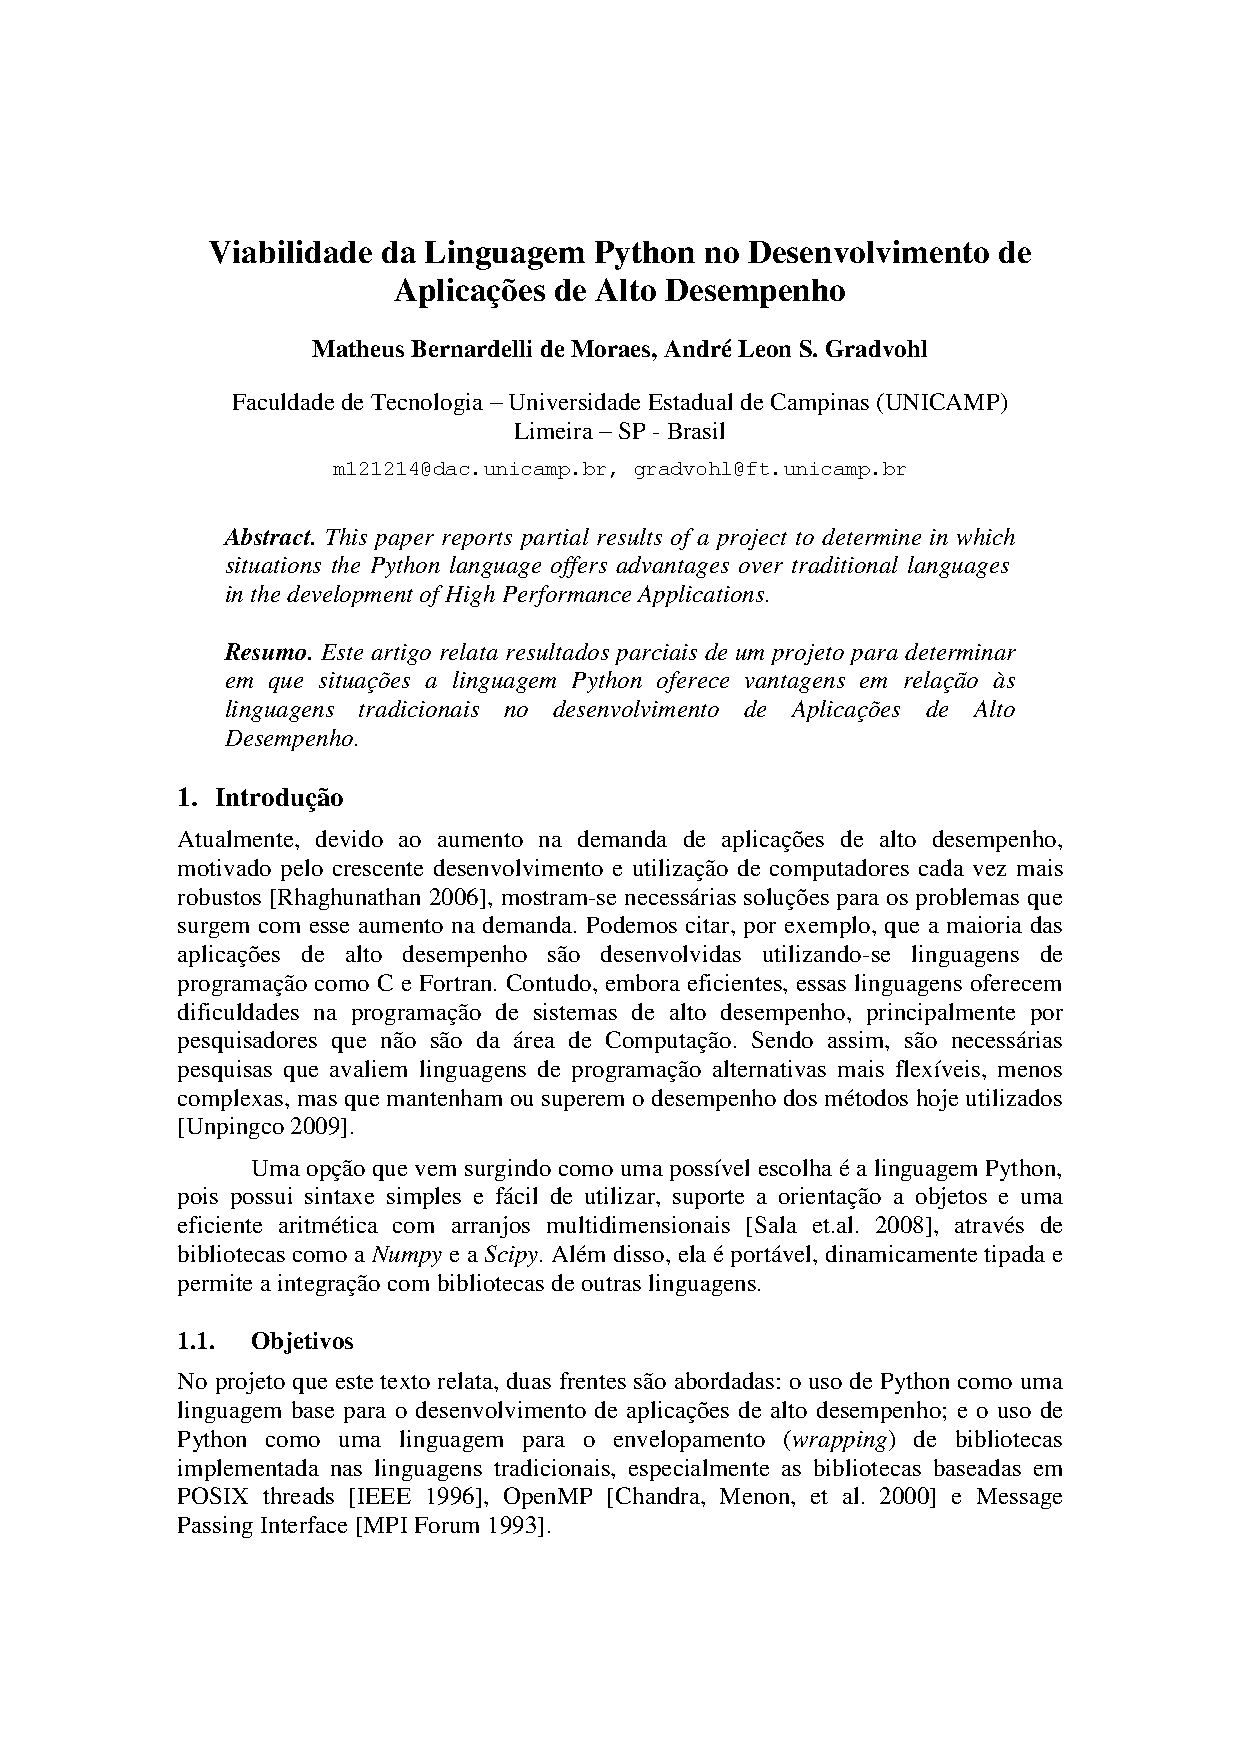
\includepdf[nup=1x2,frame,landscape=true,  width=118mm, height=195mm]{./docs/3_4_ArtigoERADMatheus}
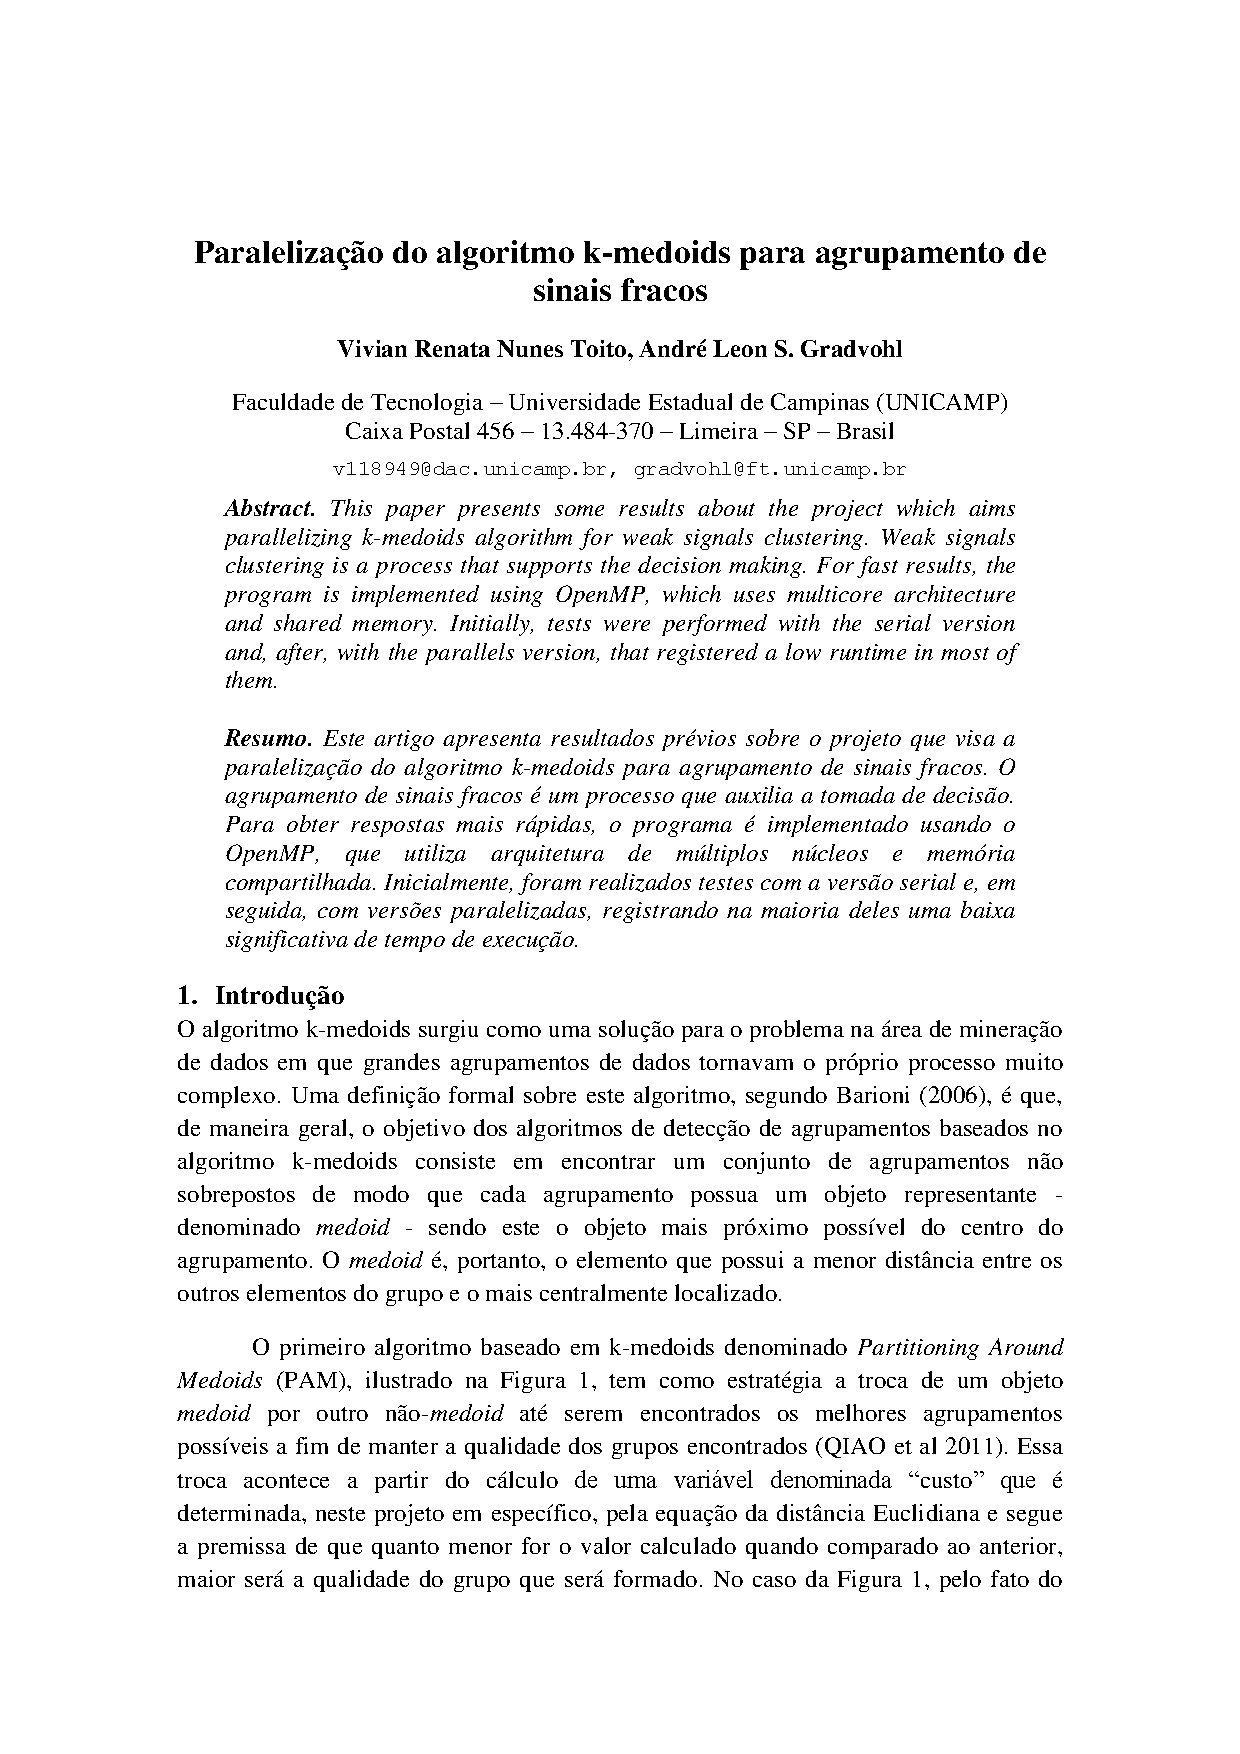
\includepdf[nup=1x2,frame,landscape=true,  width=118mm, height=195mm]{./docs/3_5_ArtigoERADVivian}
%
%
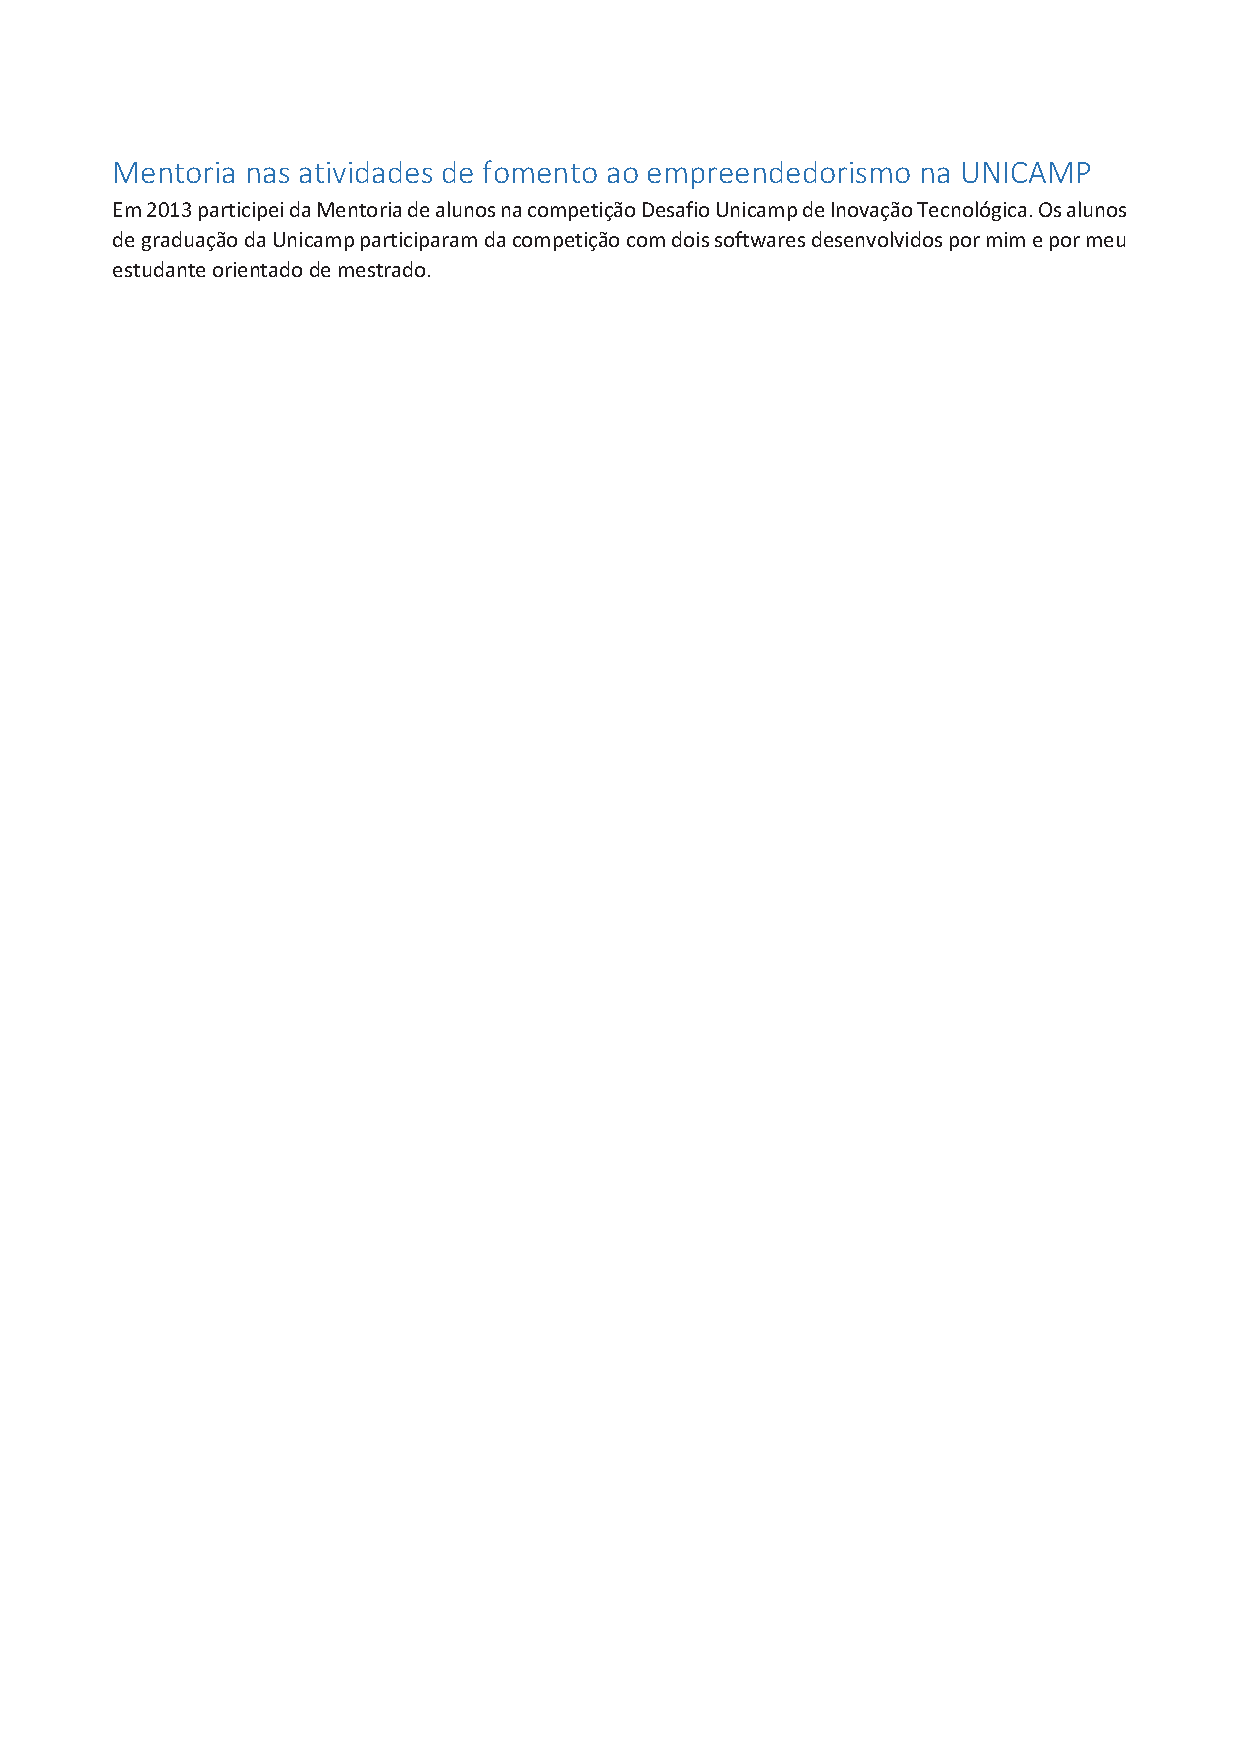
\includepdf{Mentoria.pdf}
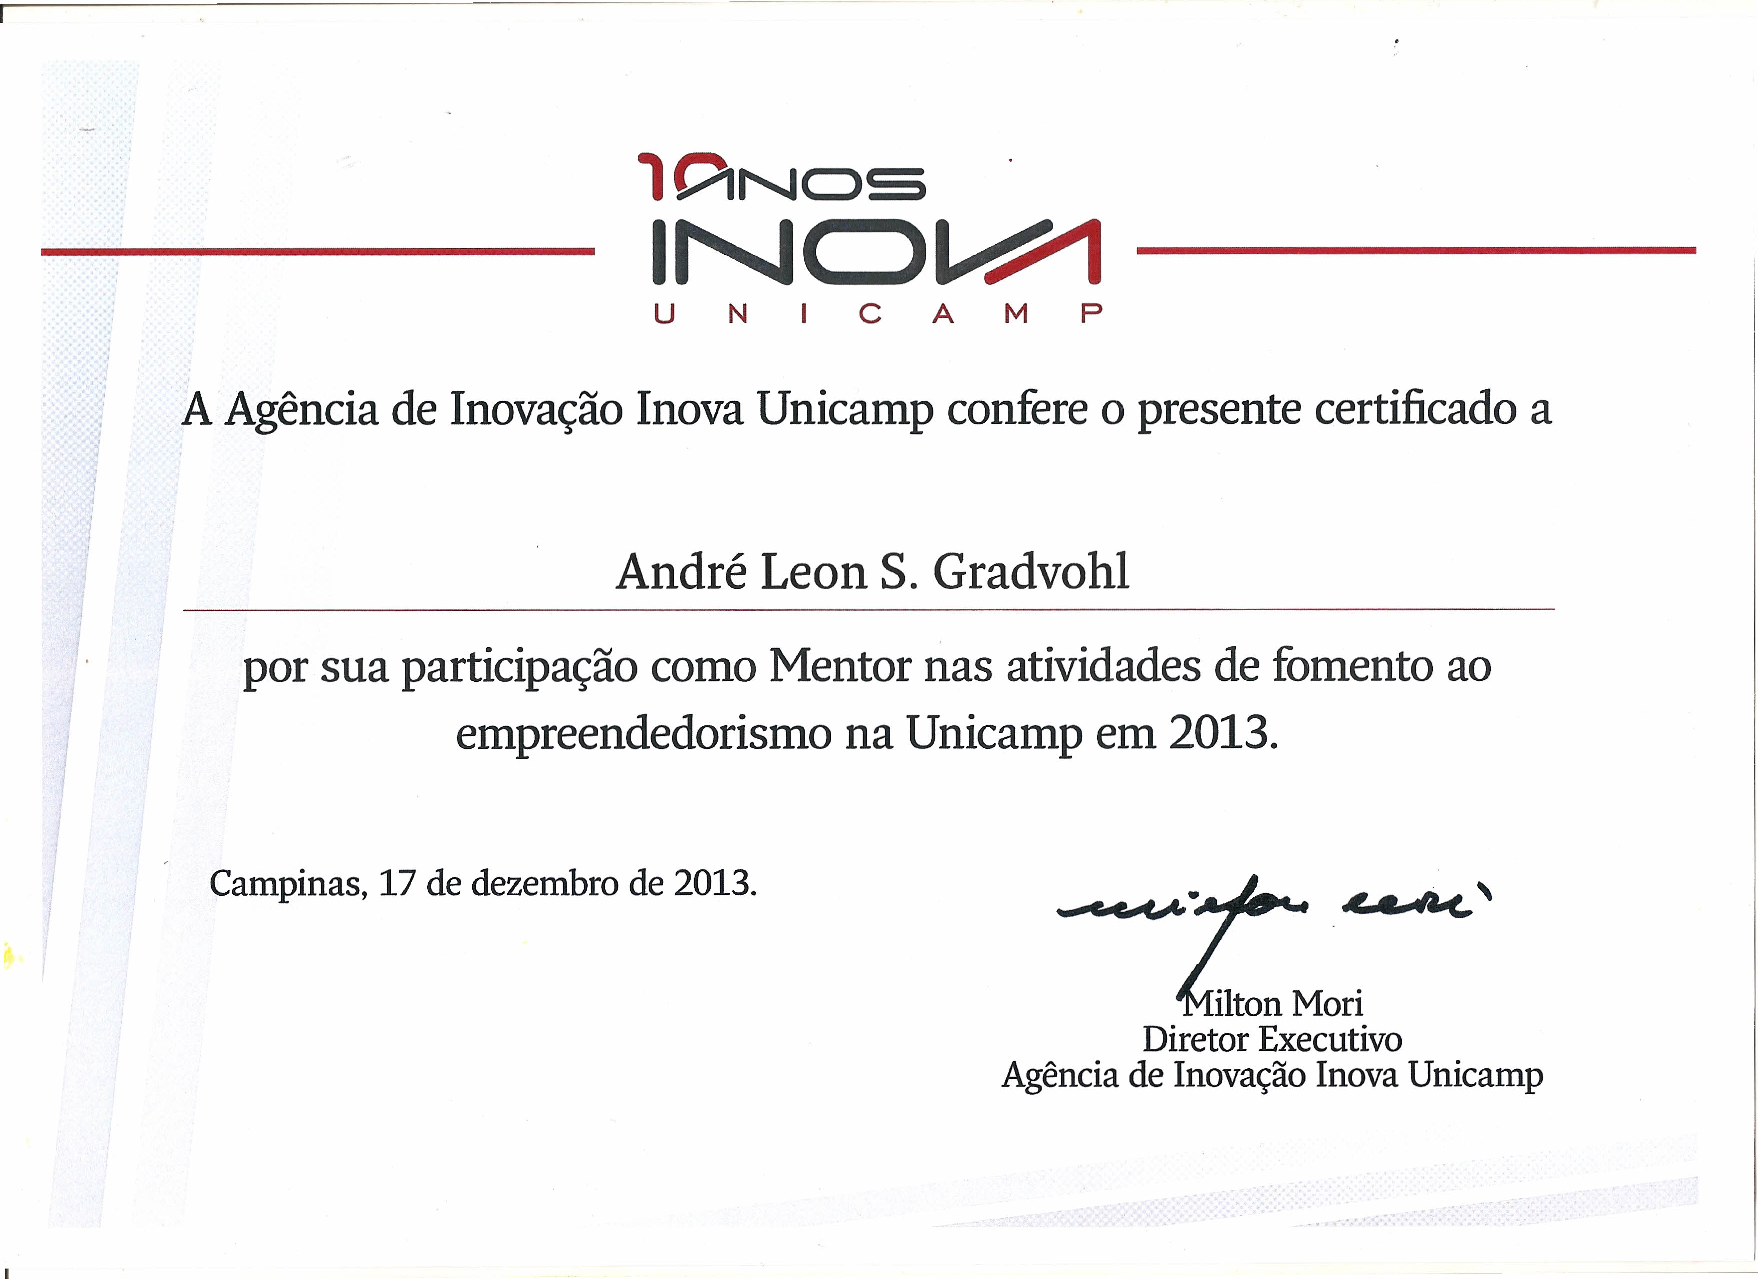
\includepdf{./docs/4_1_MentoriaInova}
%
%
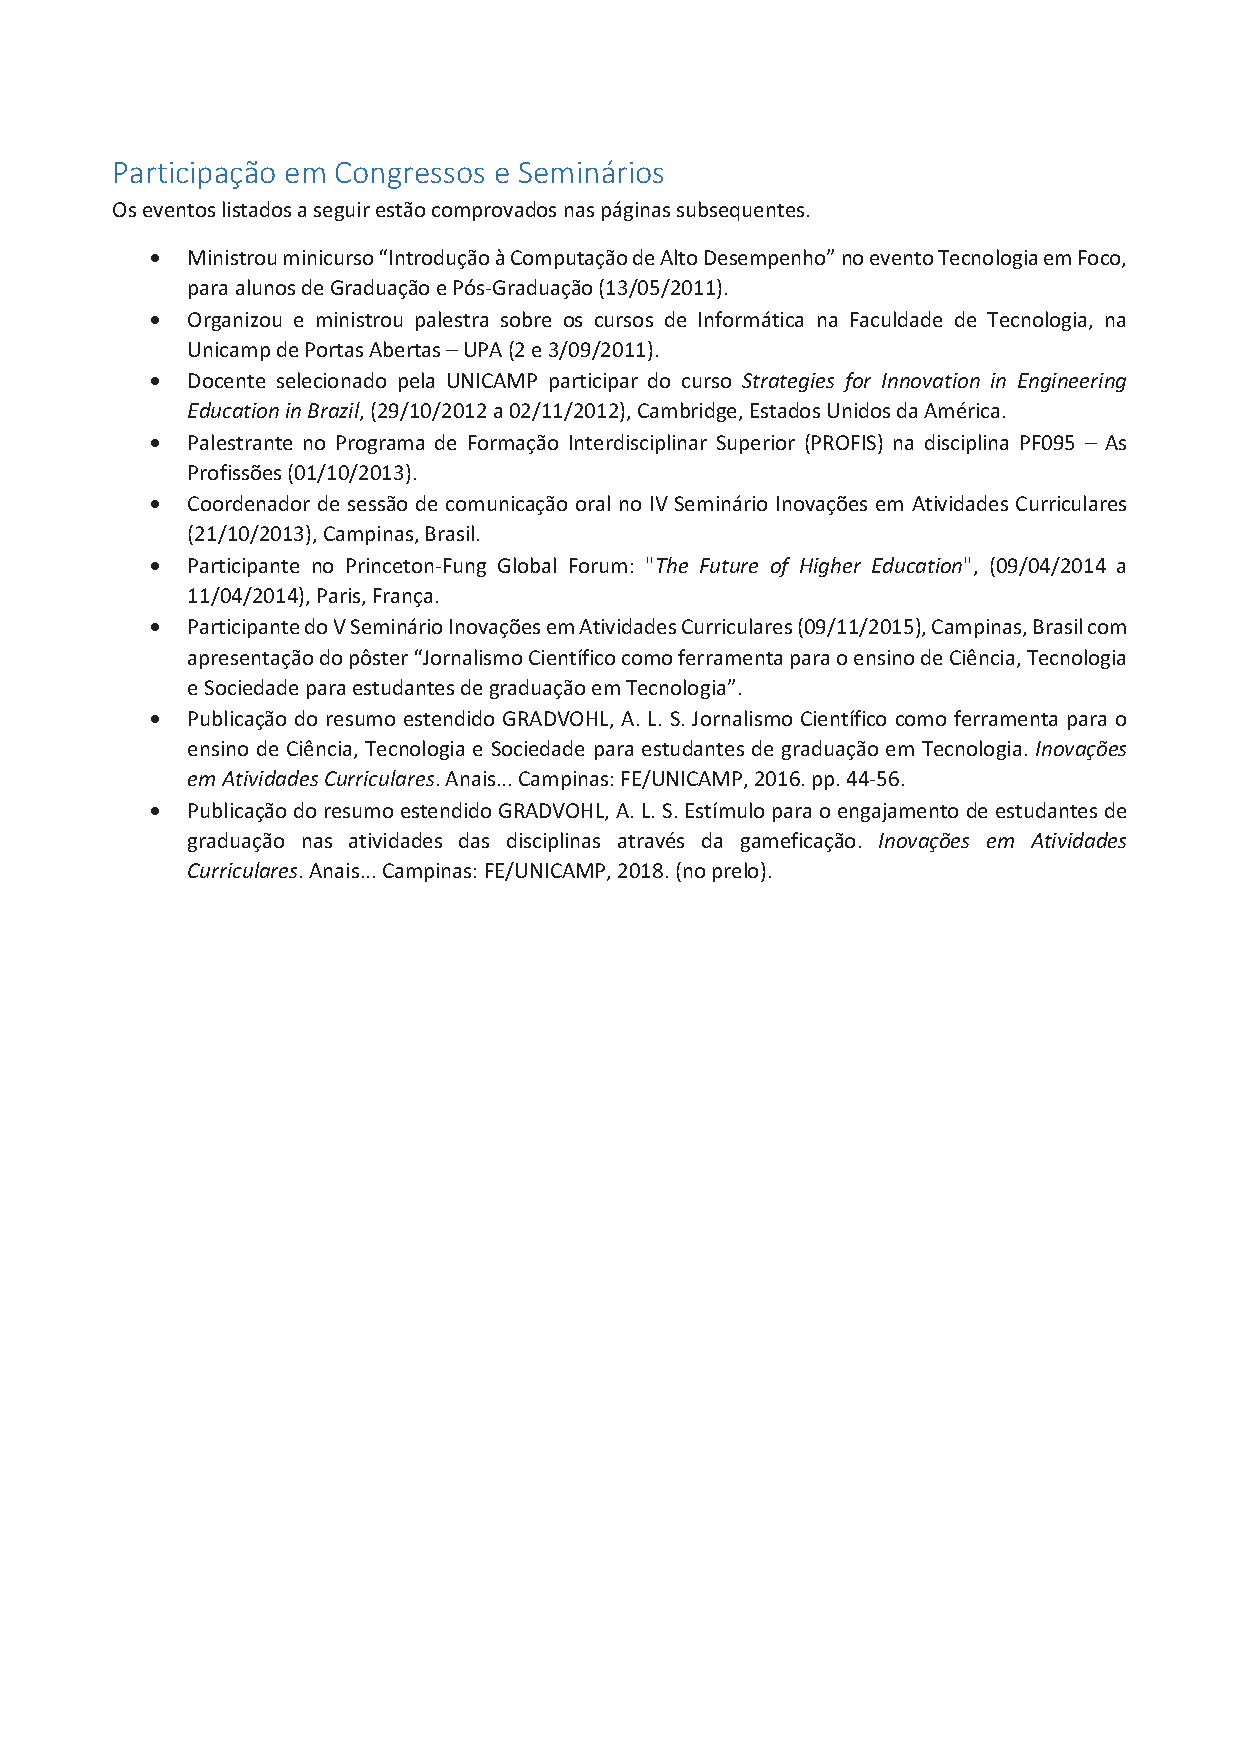
\includepdf{ParticipacaoCongressos.pdf}
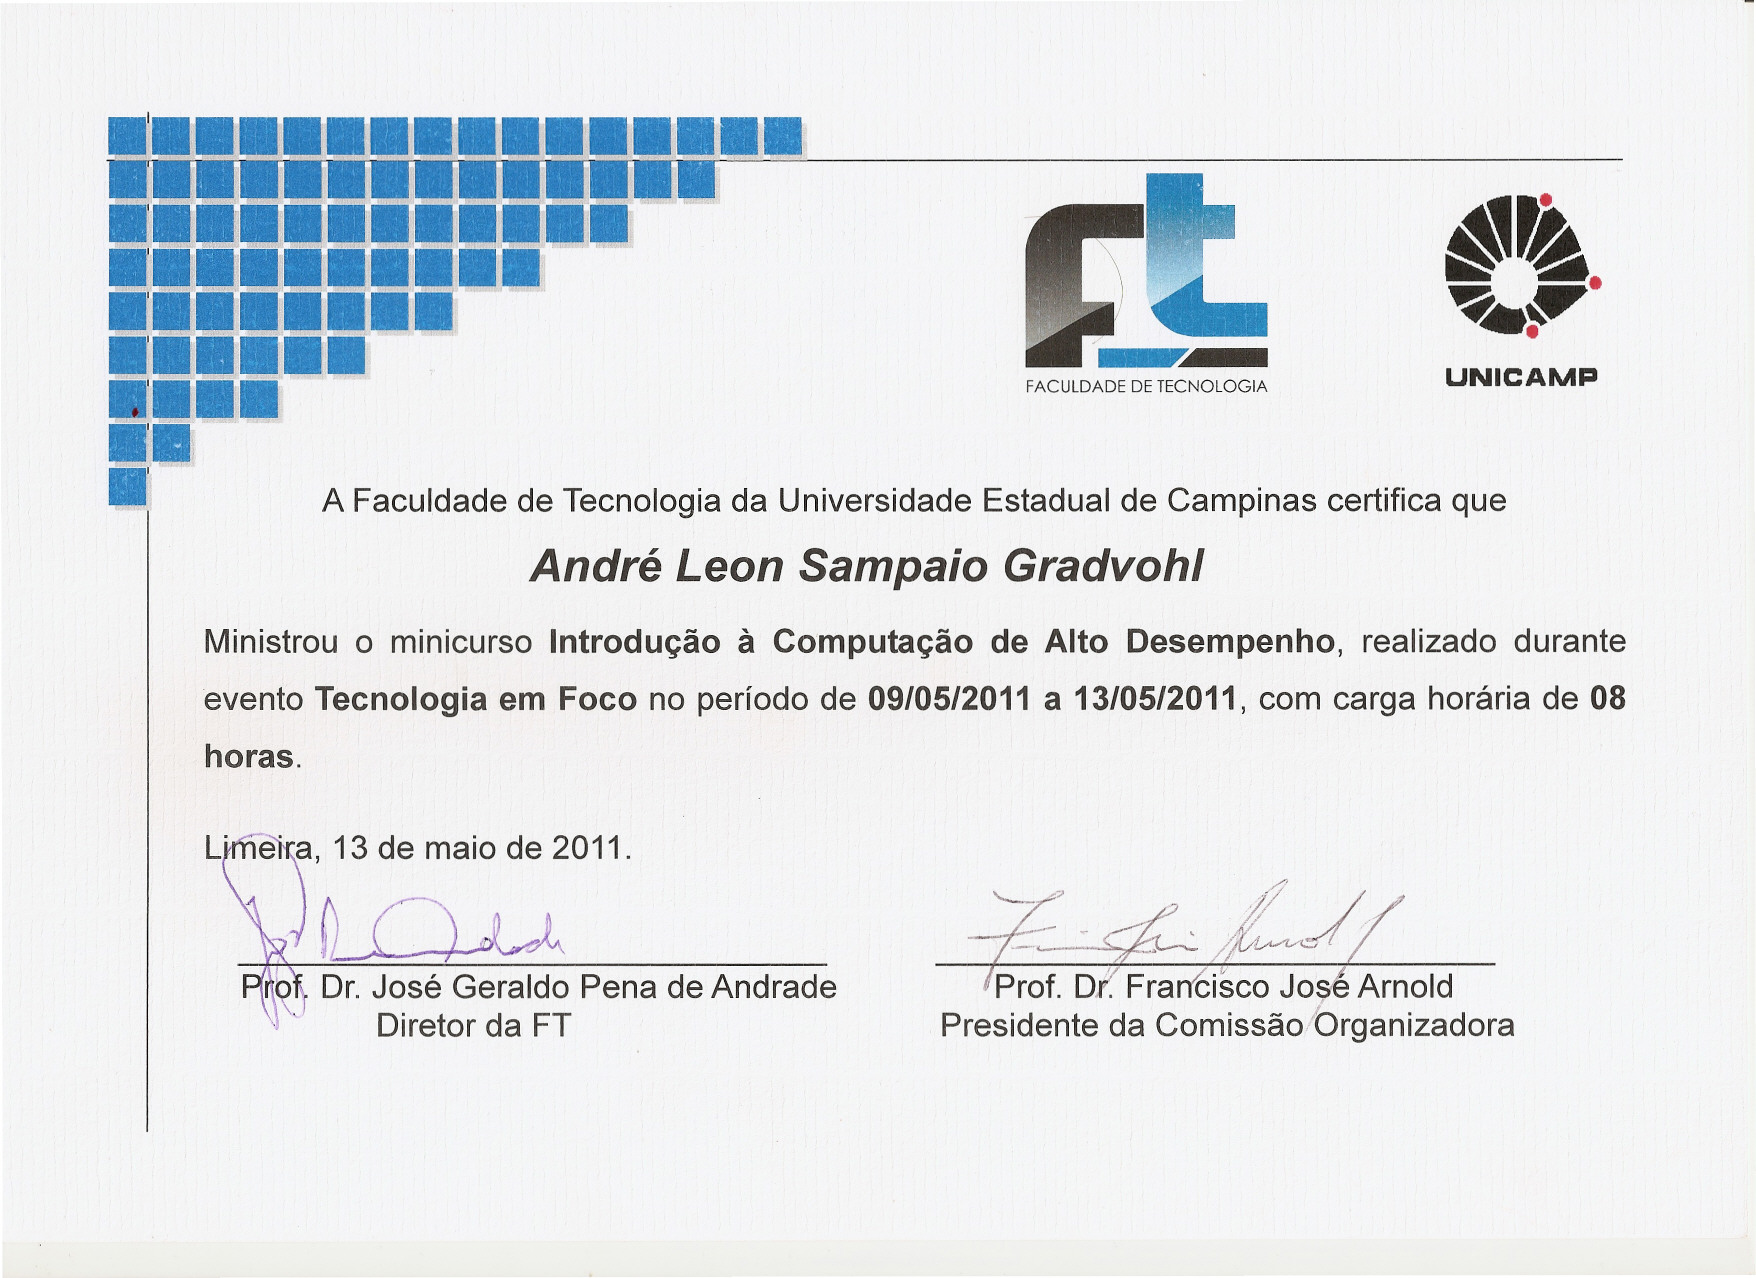
\includepdf{./docs/5_1_CertificadoMinicursoTecFoco2011}
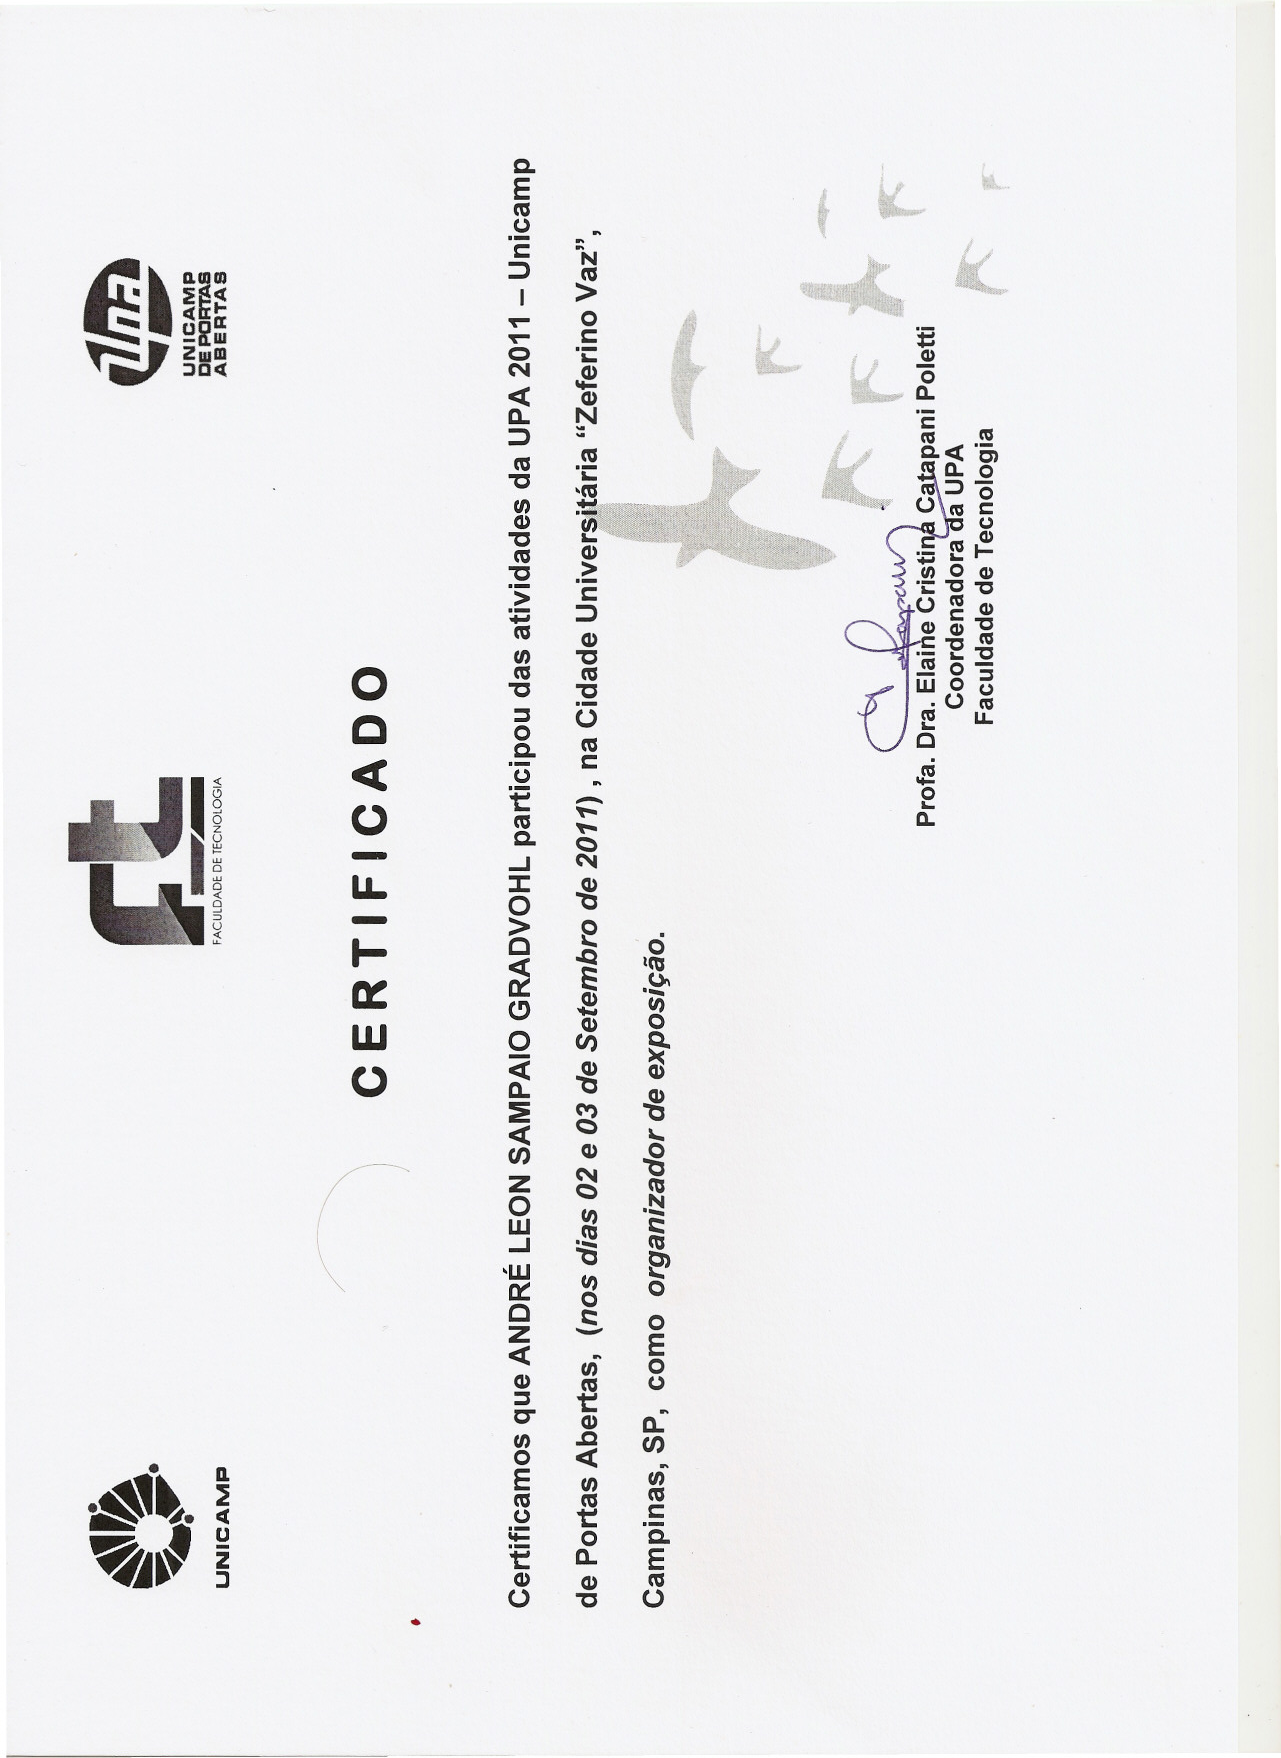
\includepdf{./docs/5_2_CertificadoOrganizacaoUPA2011}
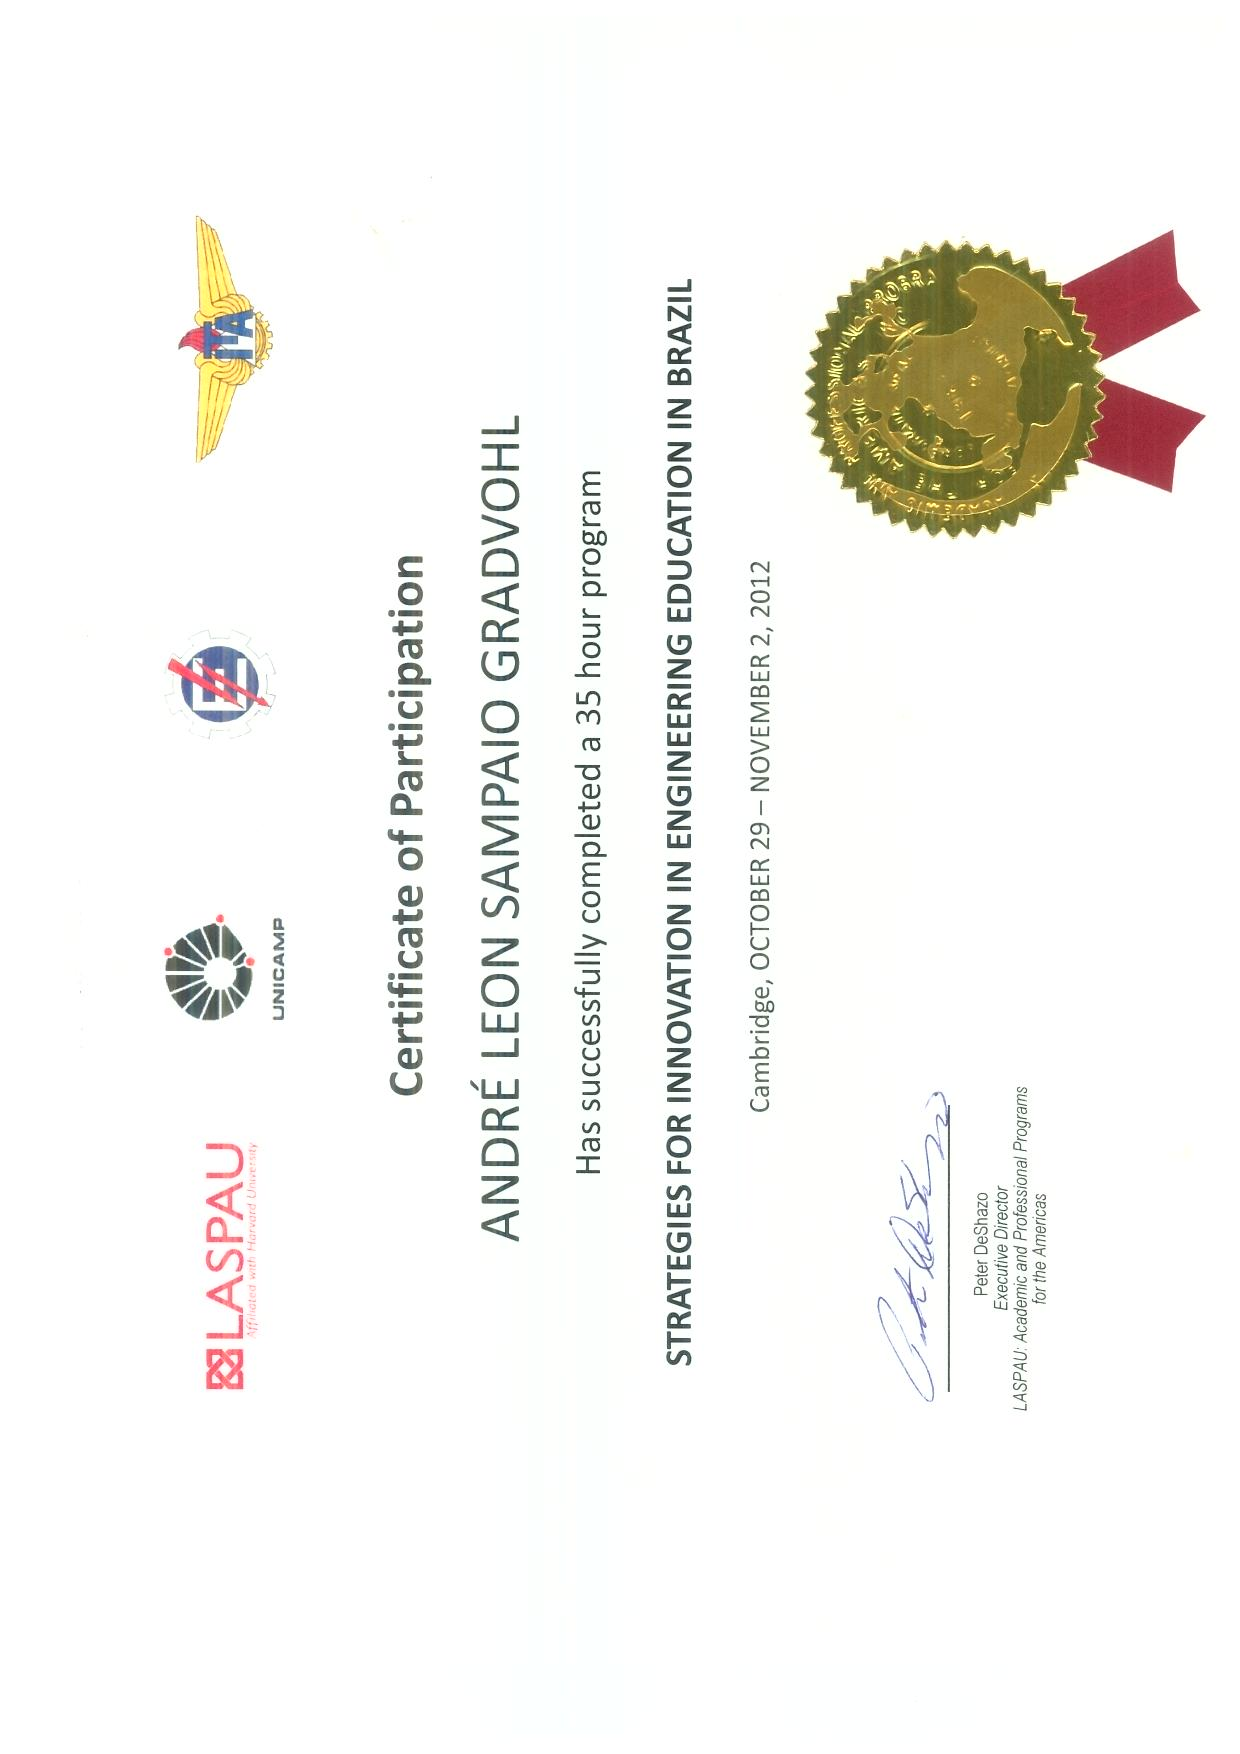
\includepdf{./docs/5_3_CertificadoLASPAU}
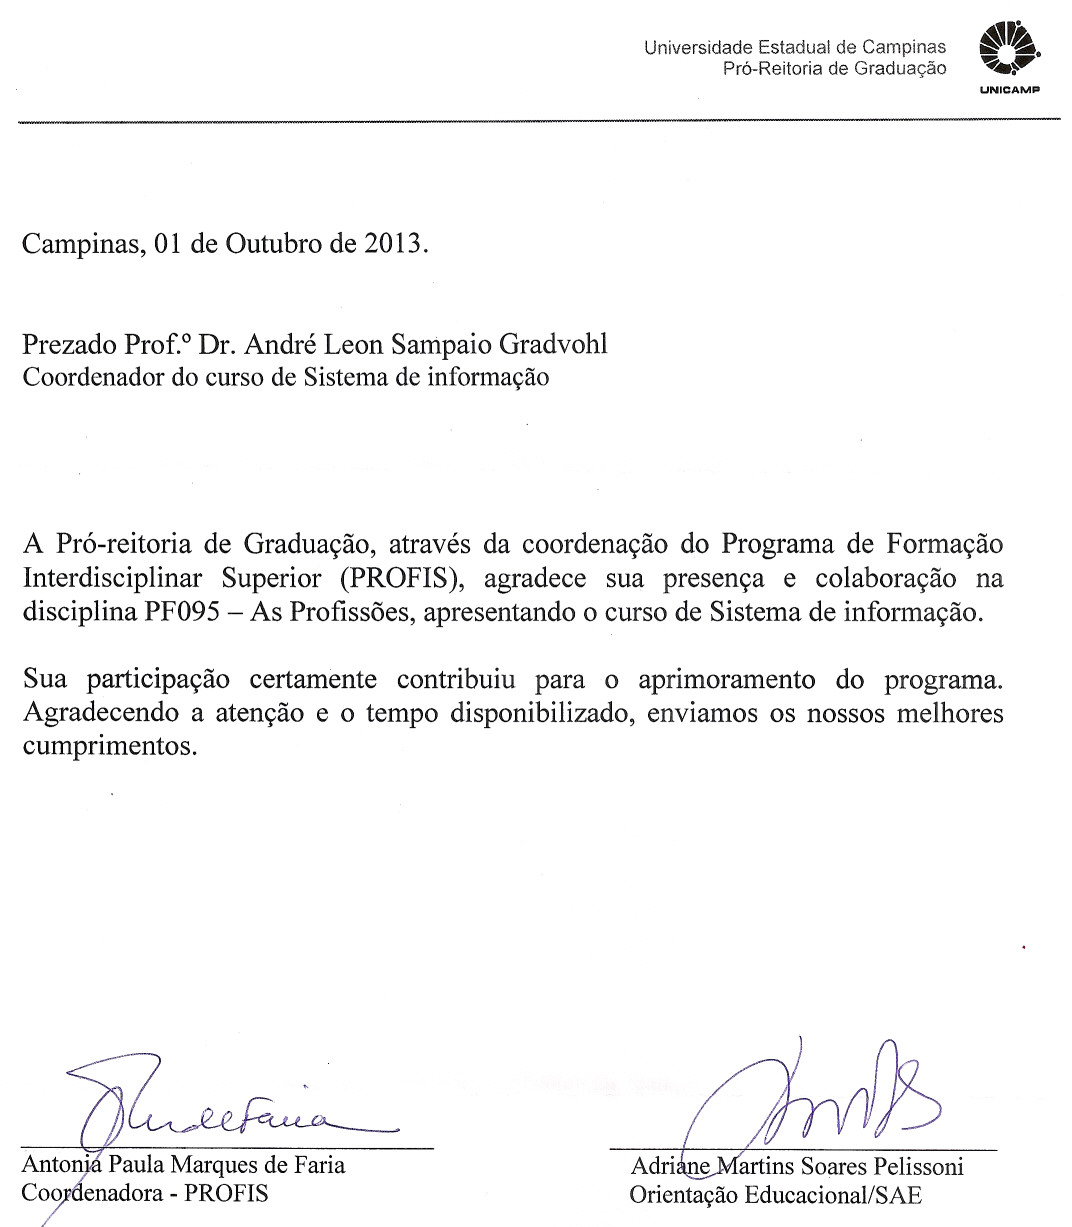
\includepdf{./docs/5_4_CertificadoPalestraProfis2013}
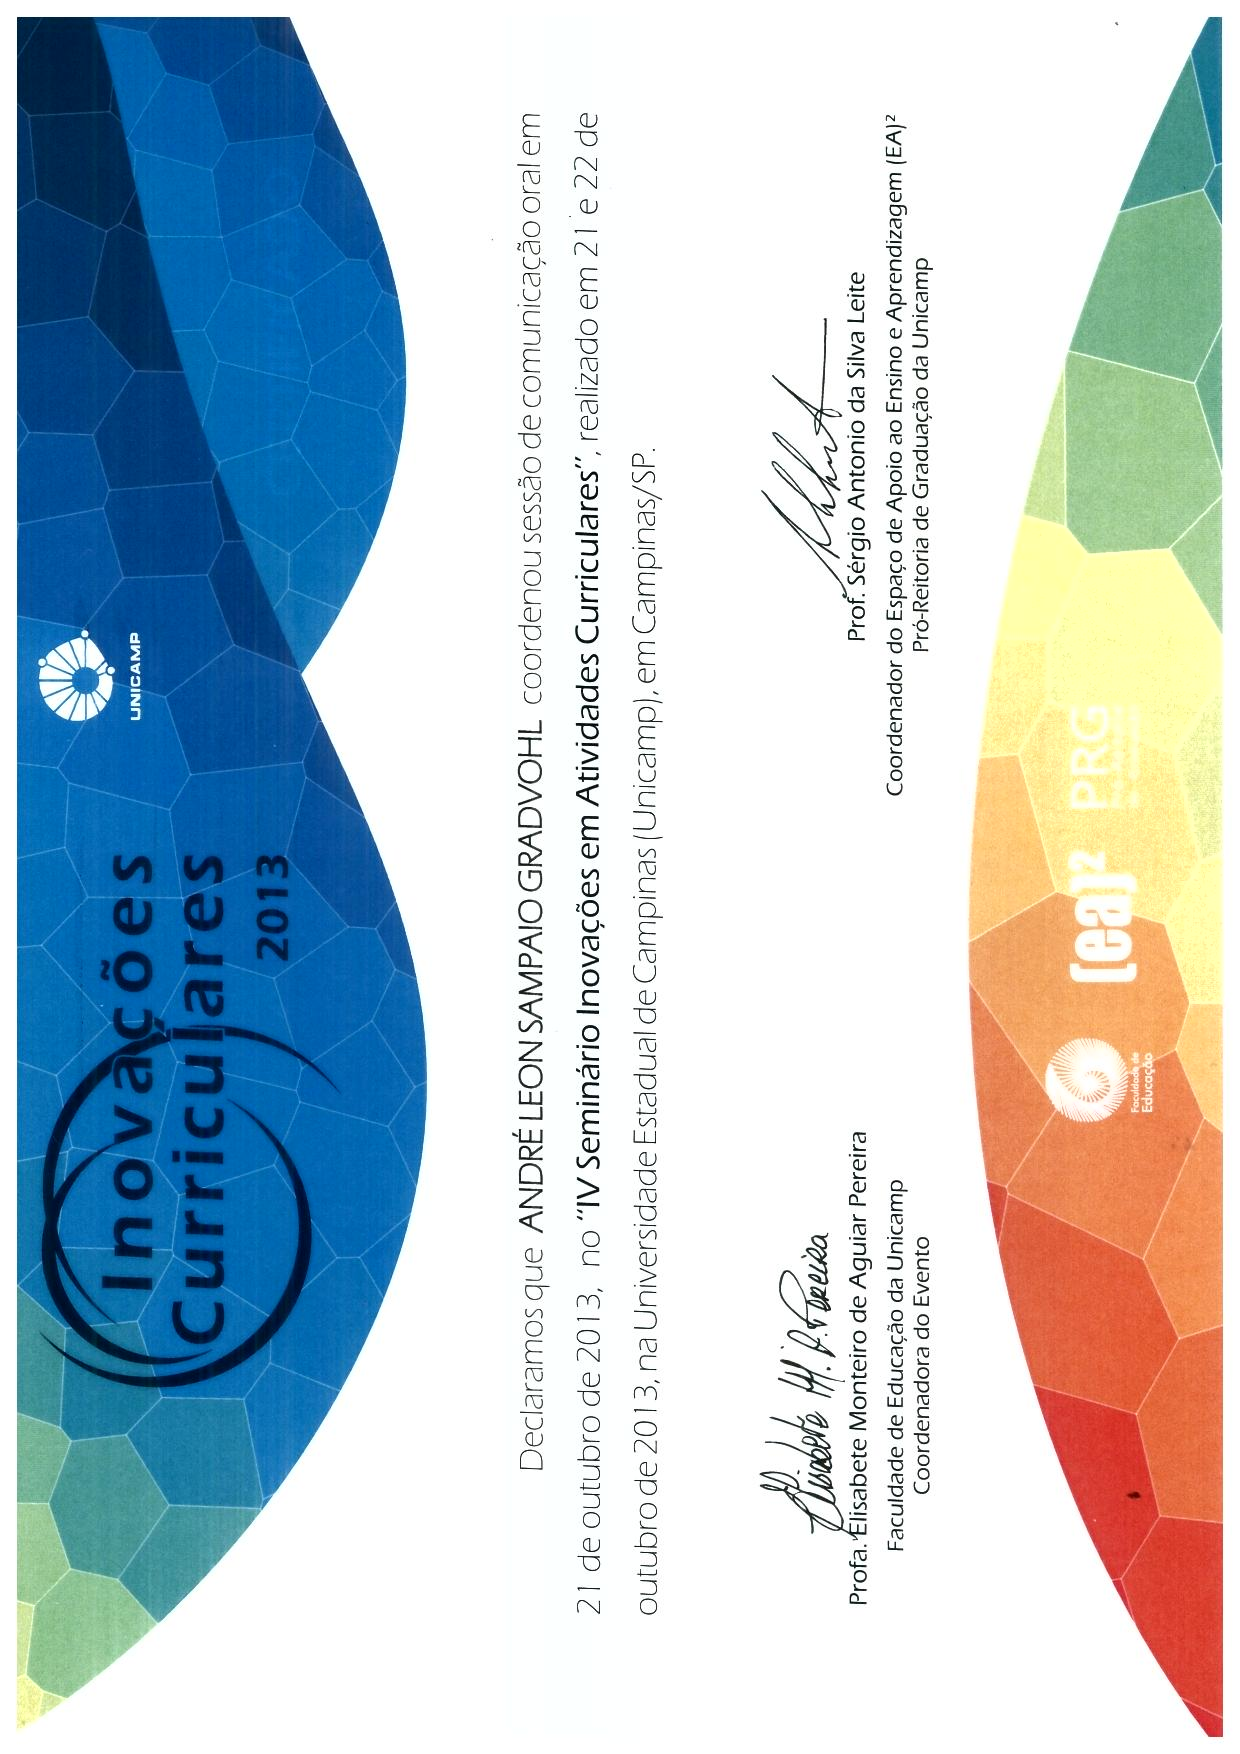
\includepdf{./docs/5_5_CertificadoCoordenadorSessaoInovacoesCurriculares2013}
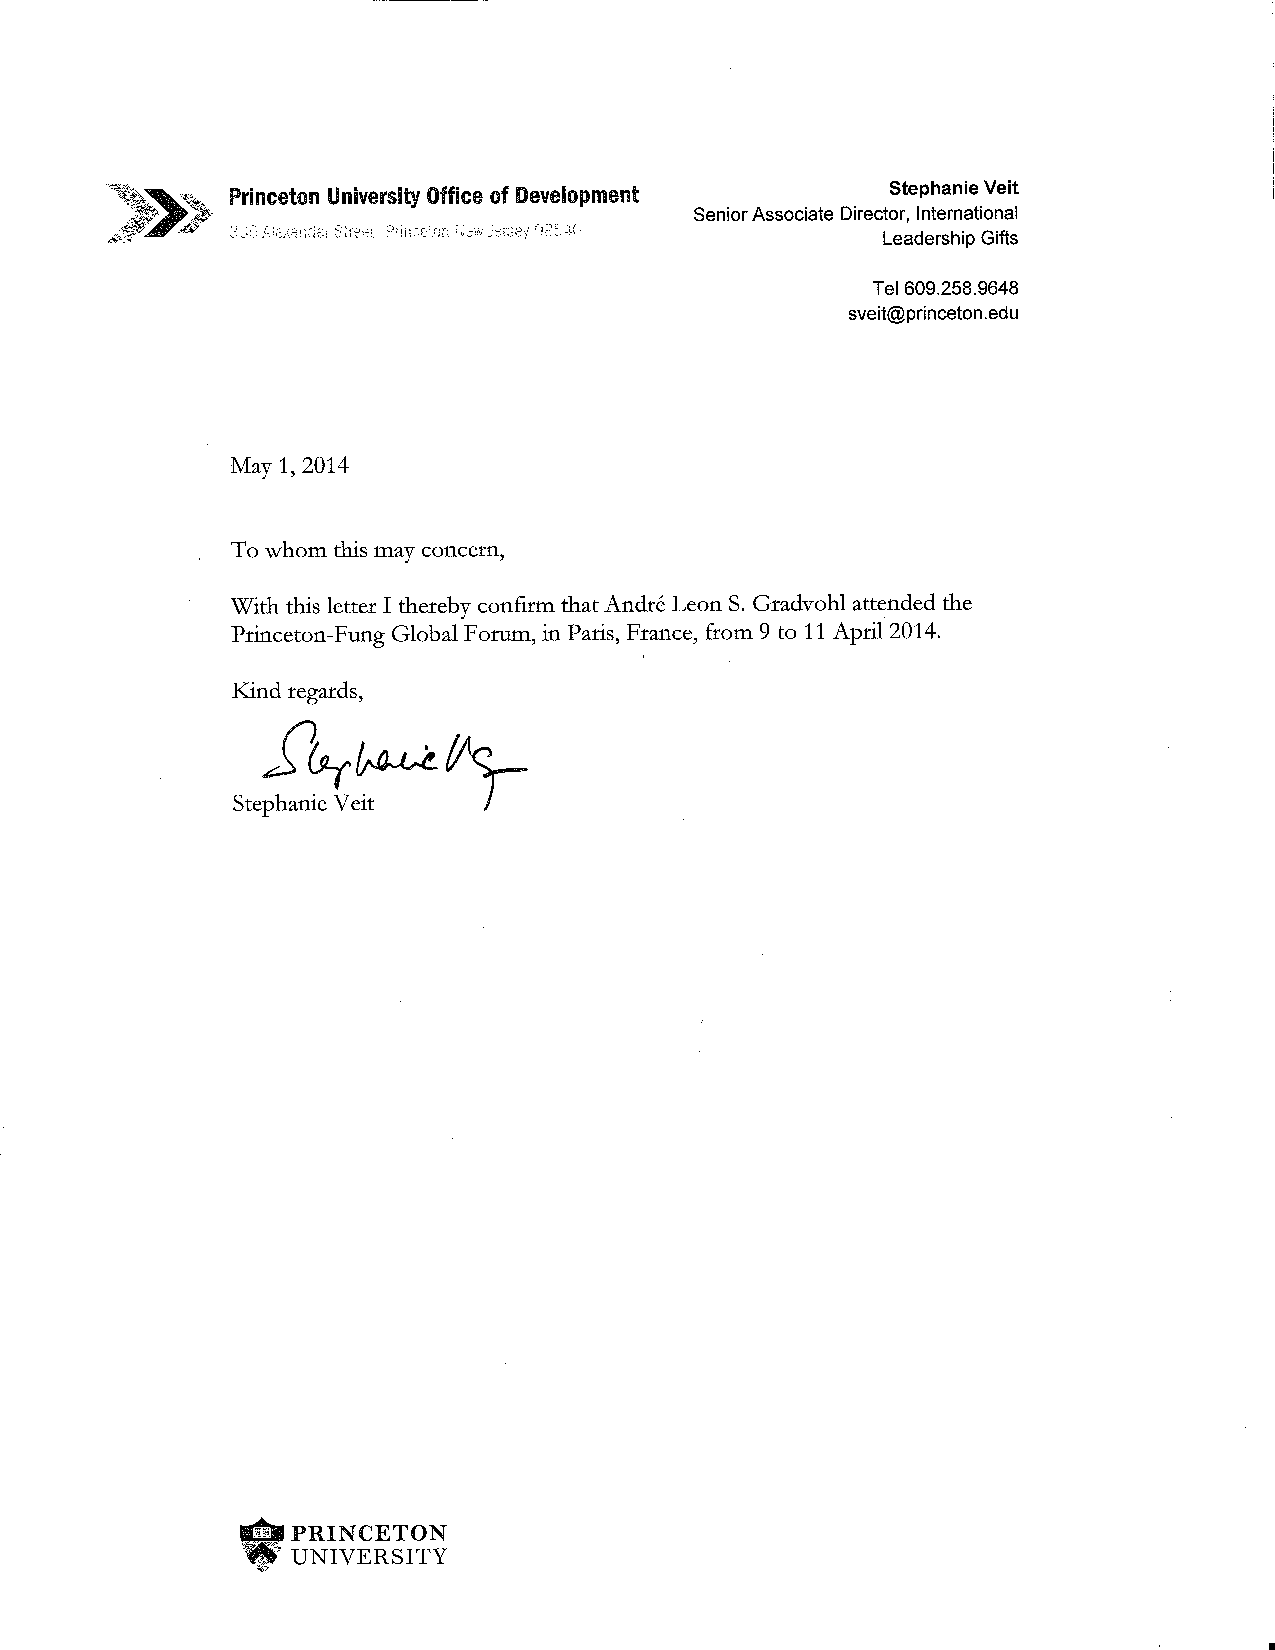
\includepdf{./docs/5_6_FungGlobalForumEducation2014}

\includepdf{./docs/5_7_CertificadoPoster_V_InovacoesCurriculares}
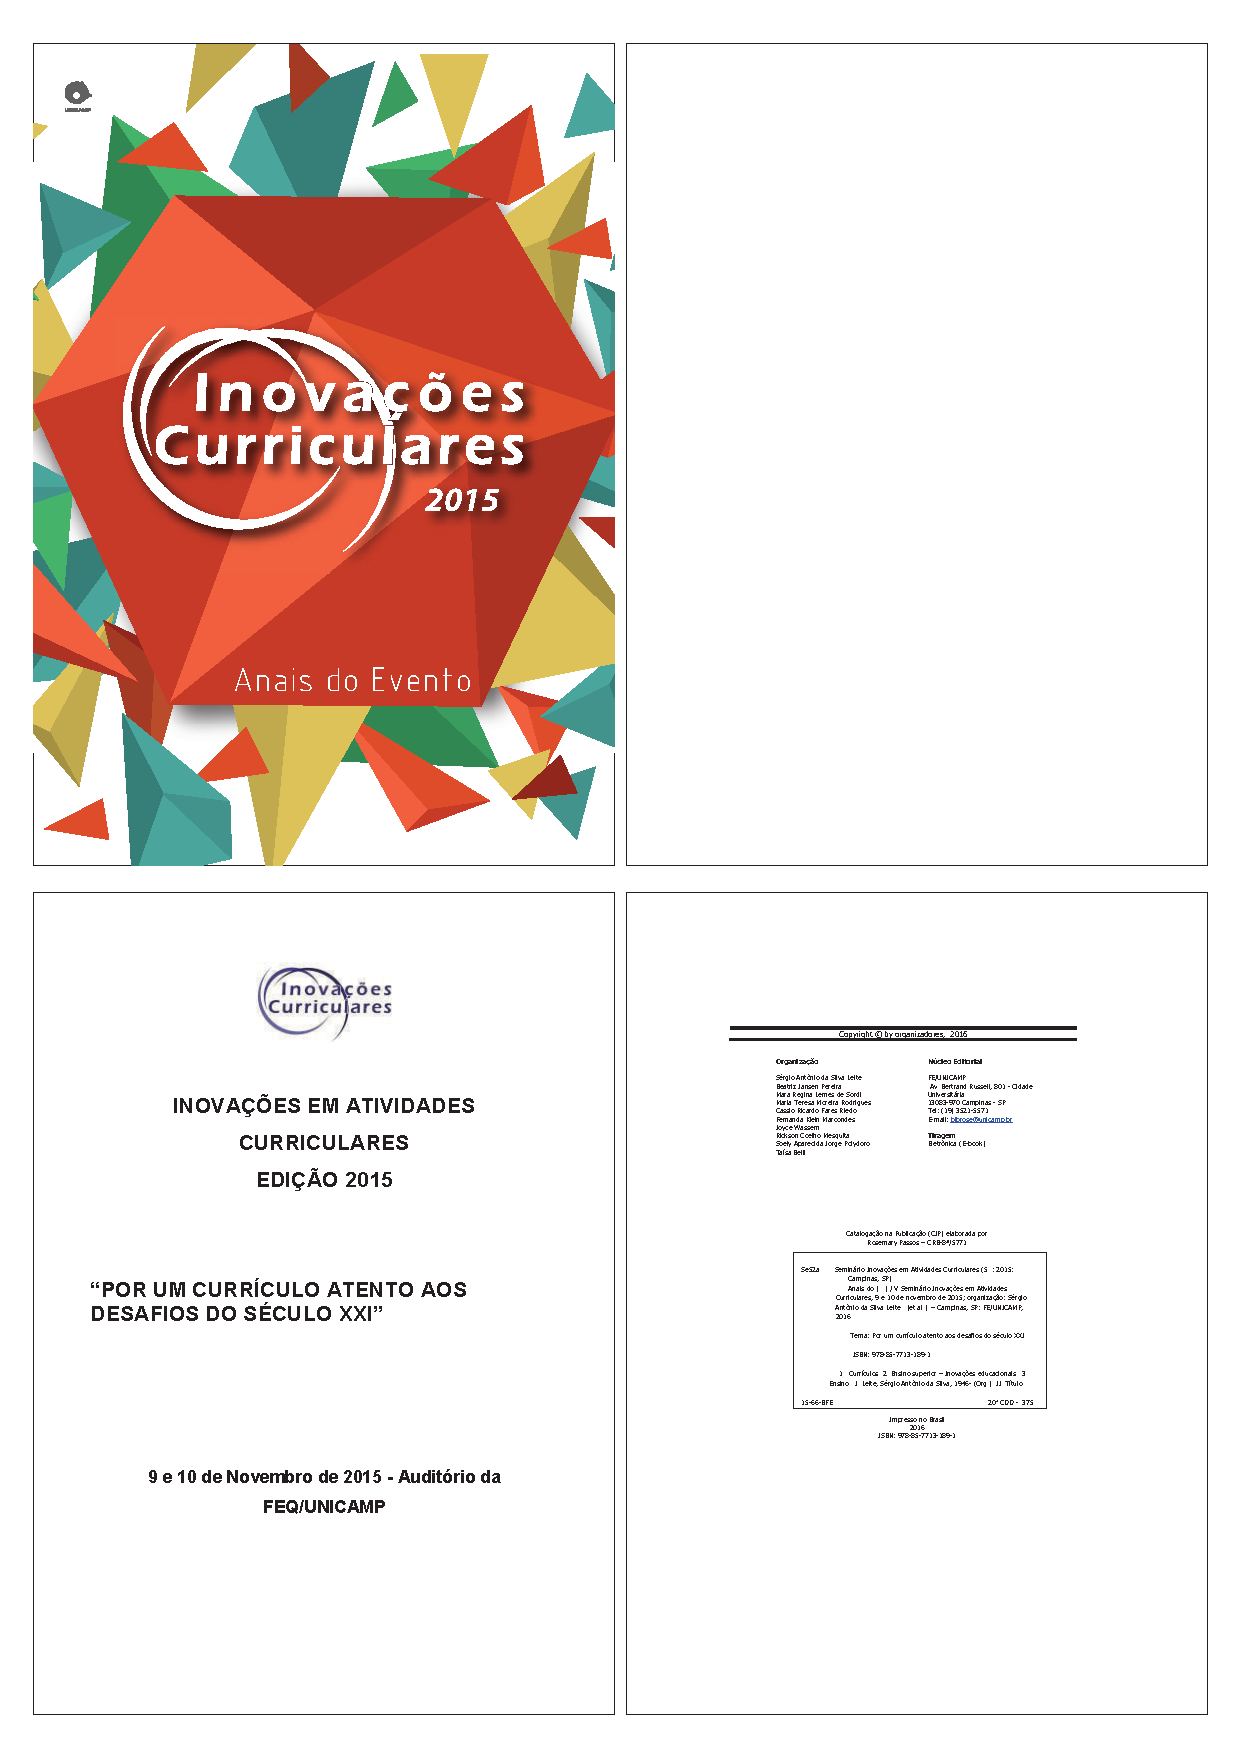
\includepdf{./docs/5_8_Artigo_em_Anais_InovacoesCurriculares_2015_4x4}
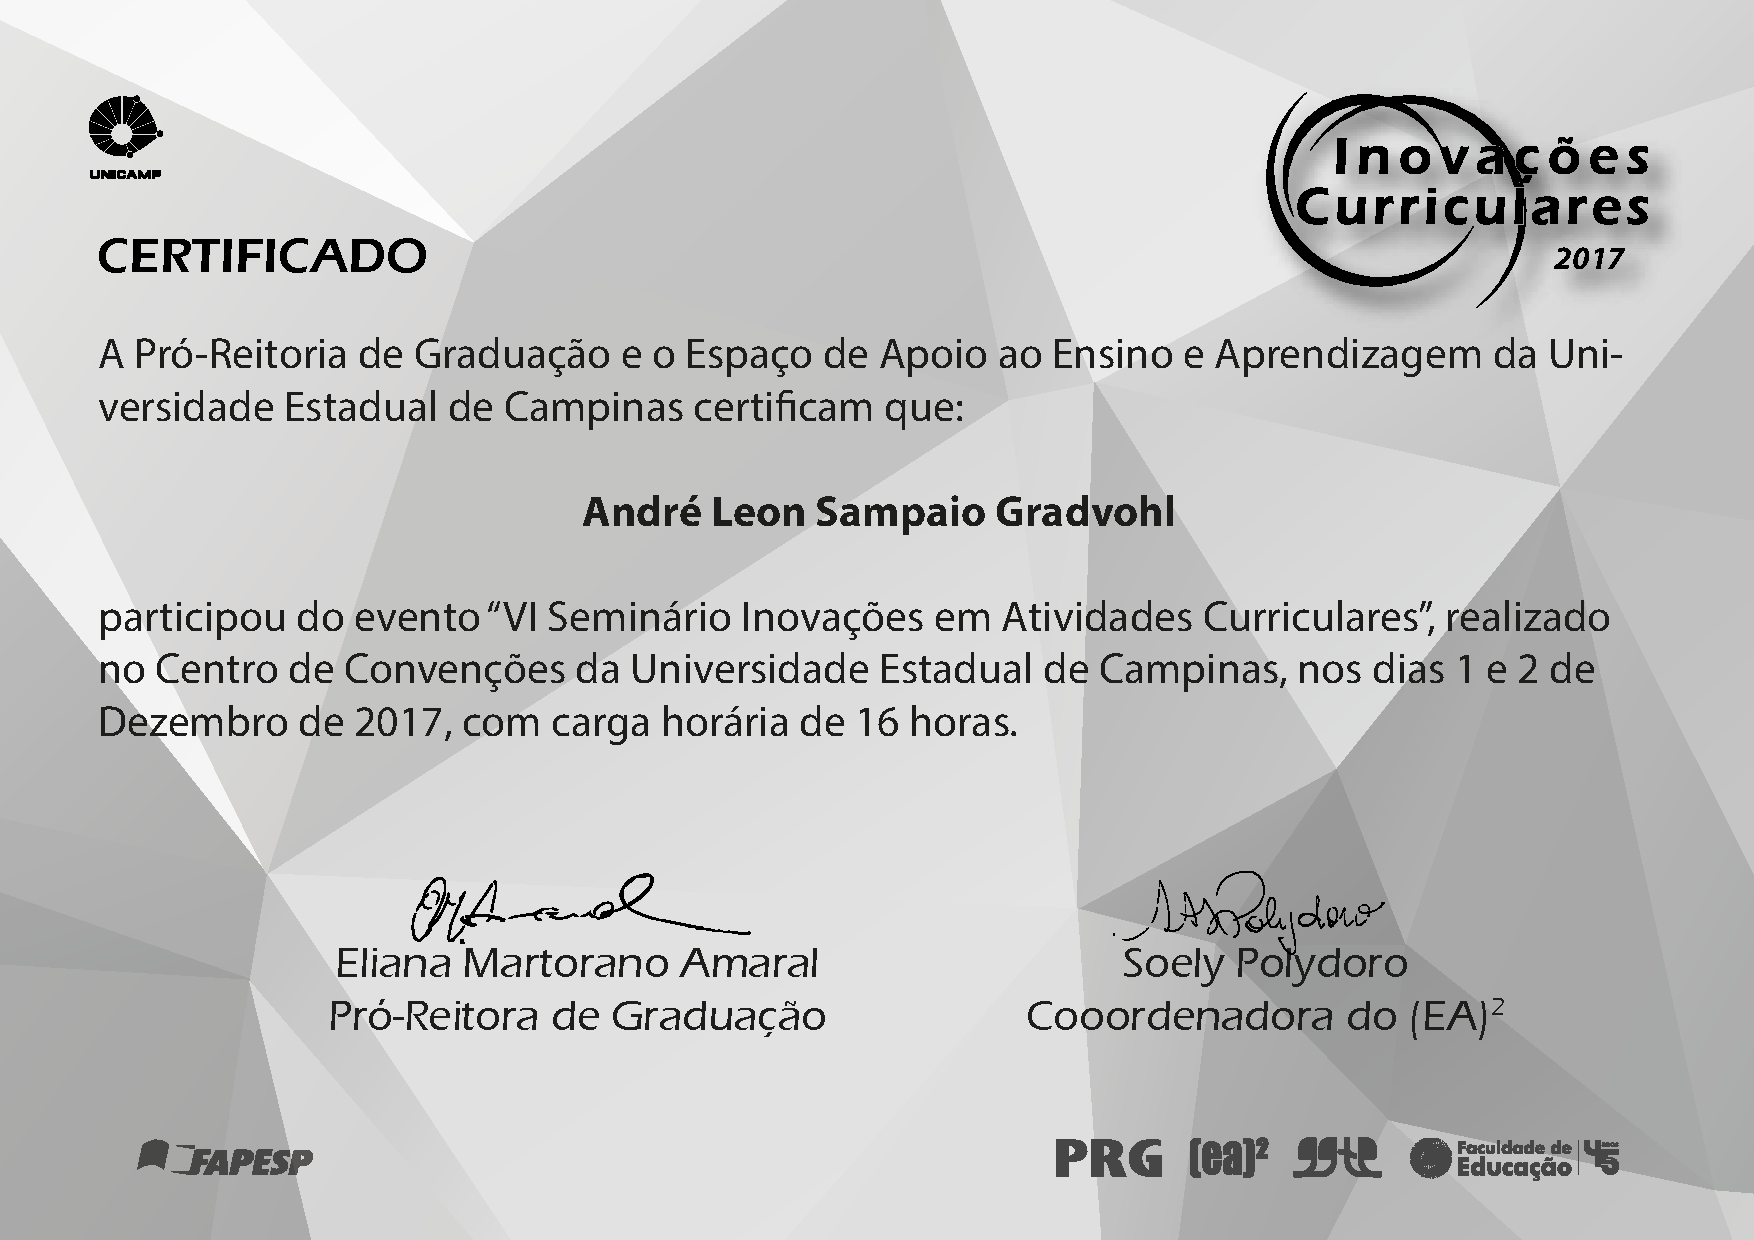
\includepdf{./docs/5_9_1_CertificadoInovacoesCurriculares2017}
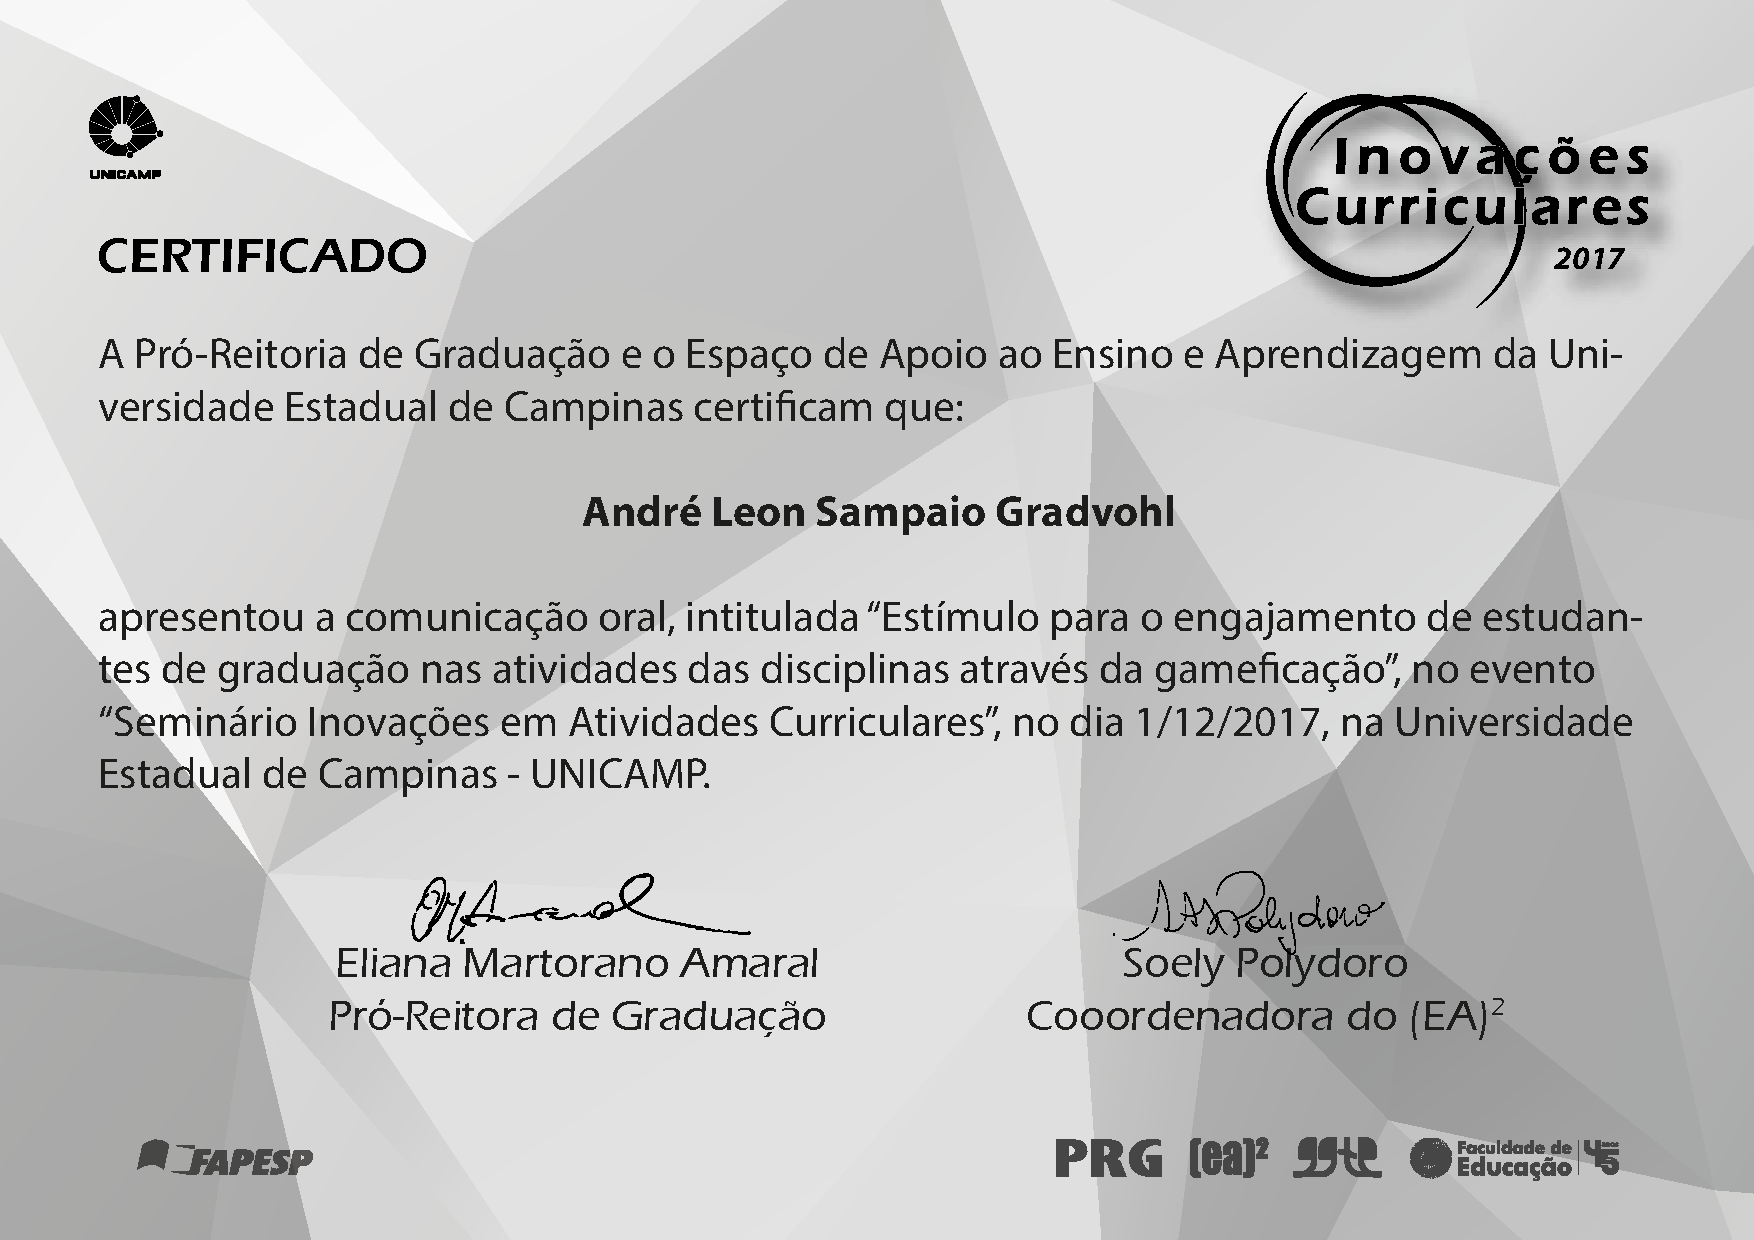
\includepdf{./docs/5_9_2_CertificadoInovacoesCurriculares2017}
%
%
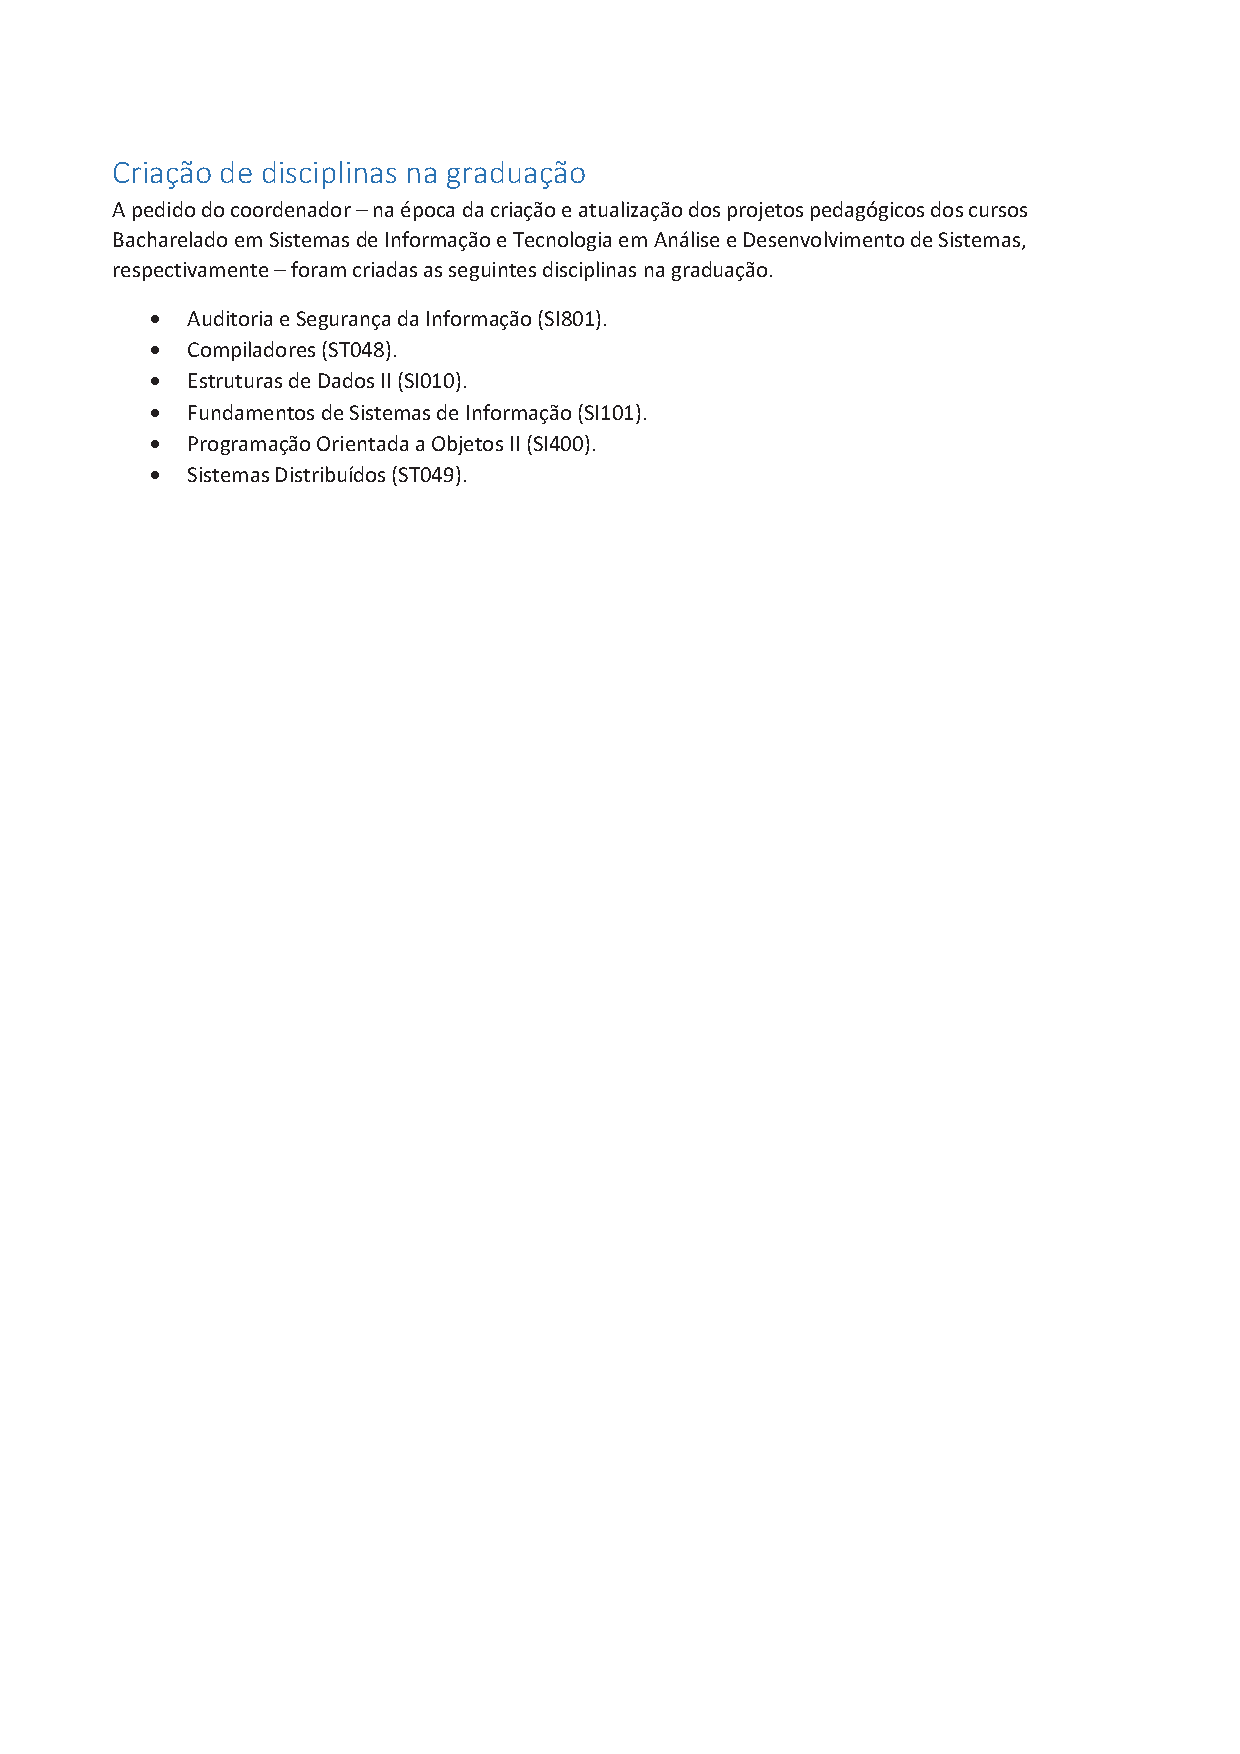
\includepdf{CriacaoDisciplinas.pdf}
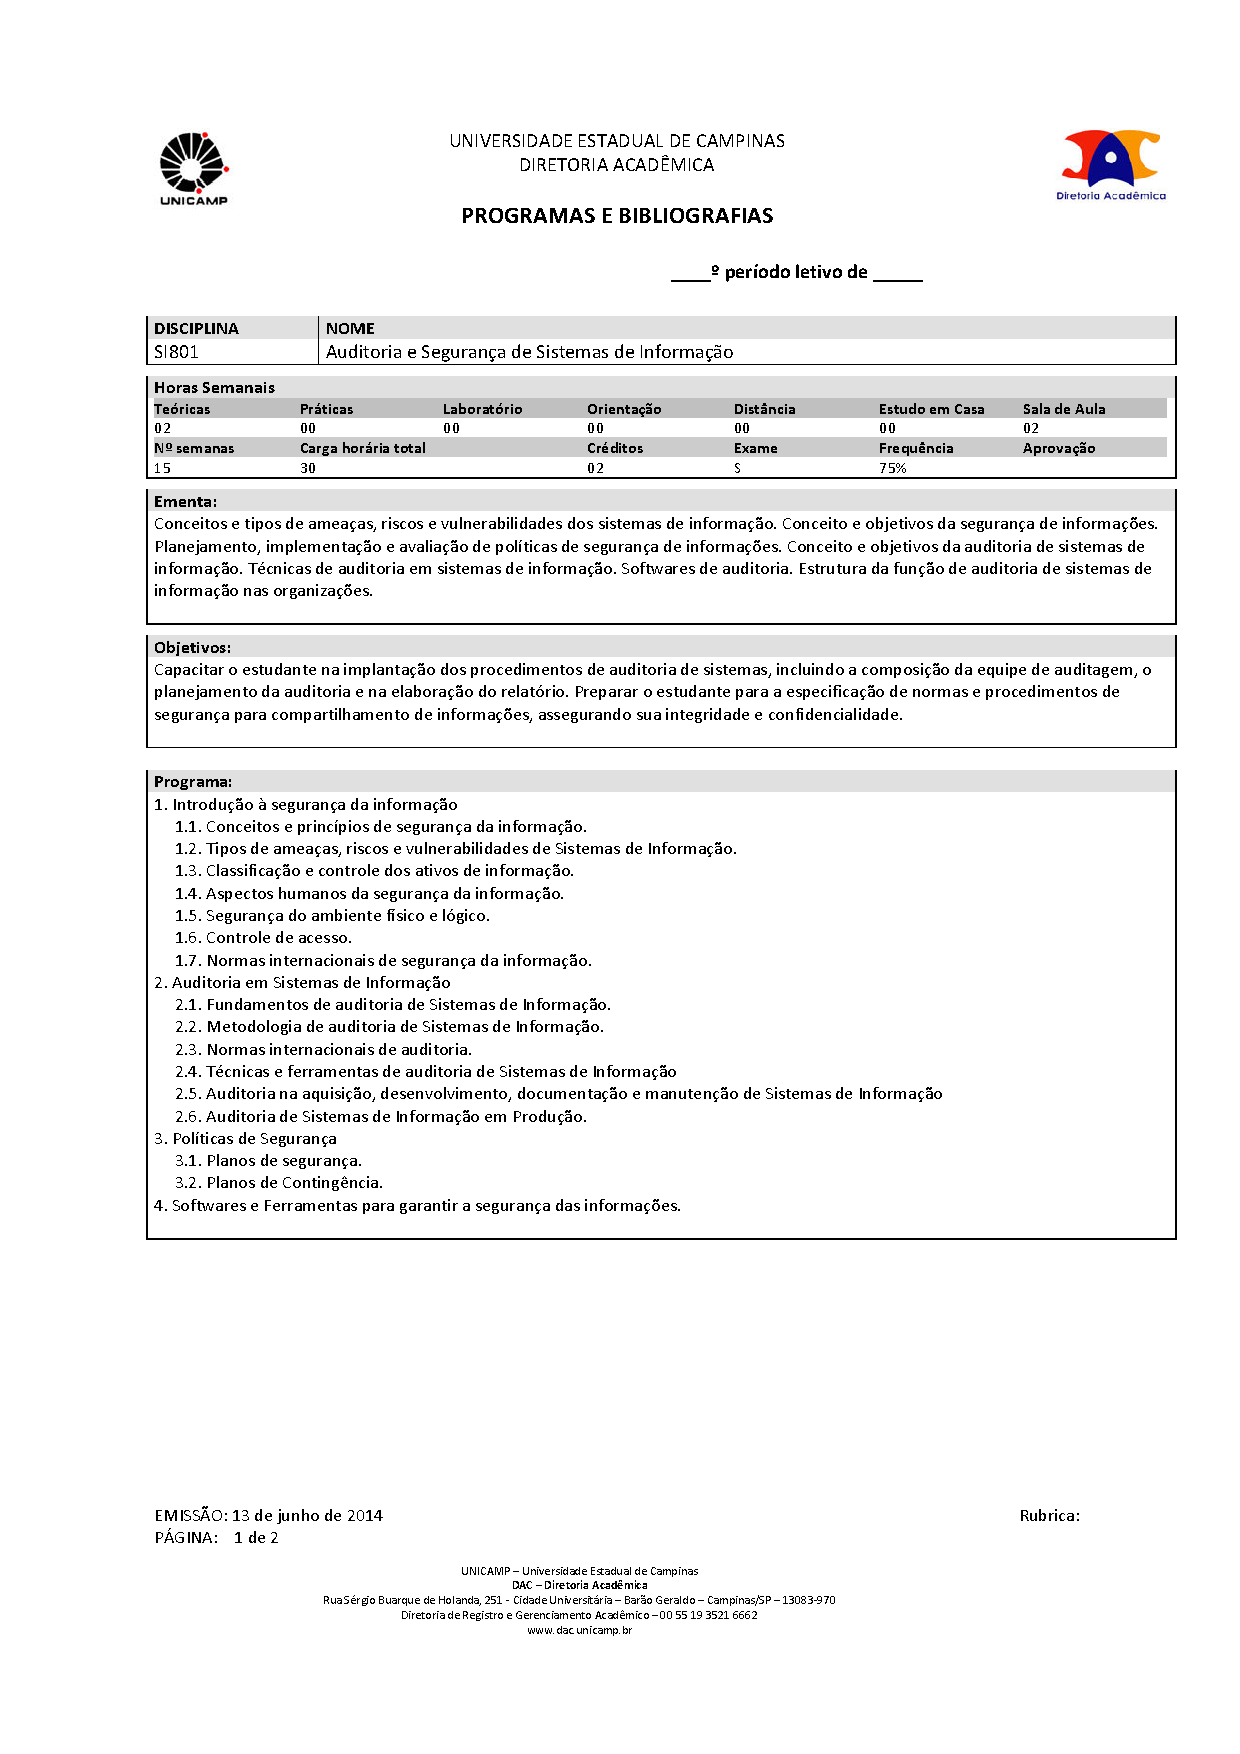
\includepdf{./docs/6_1_ProgramaDACAuditoriaSegurancaSistemasInformacao}
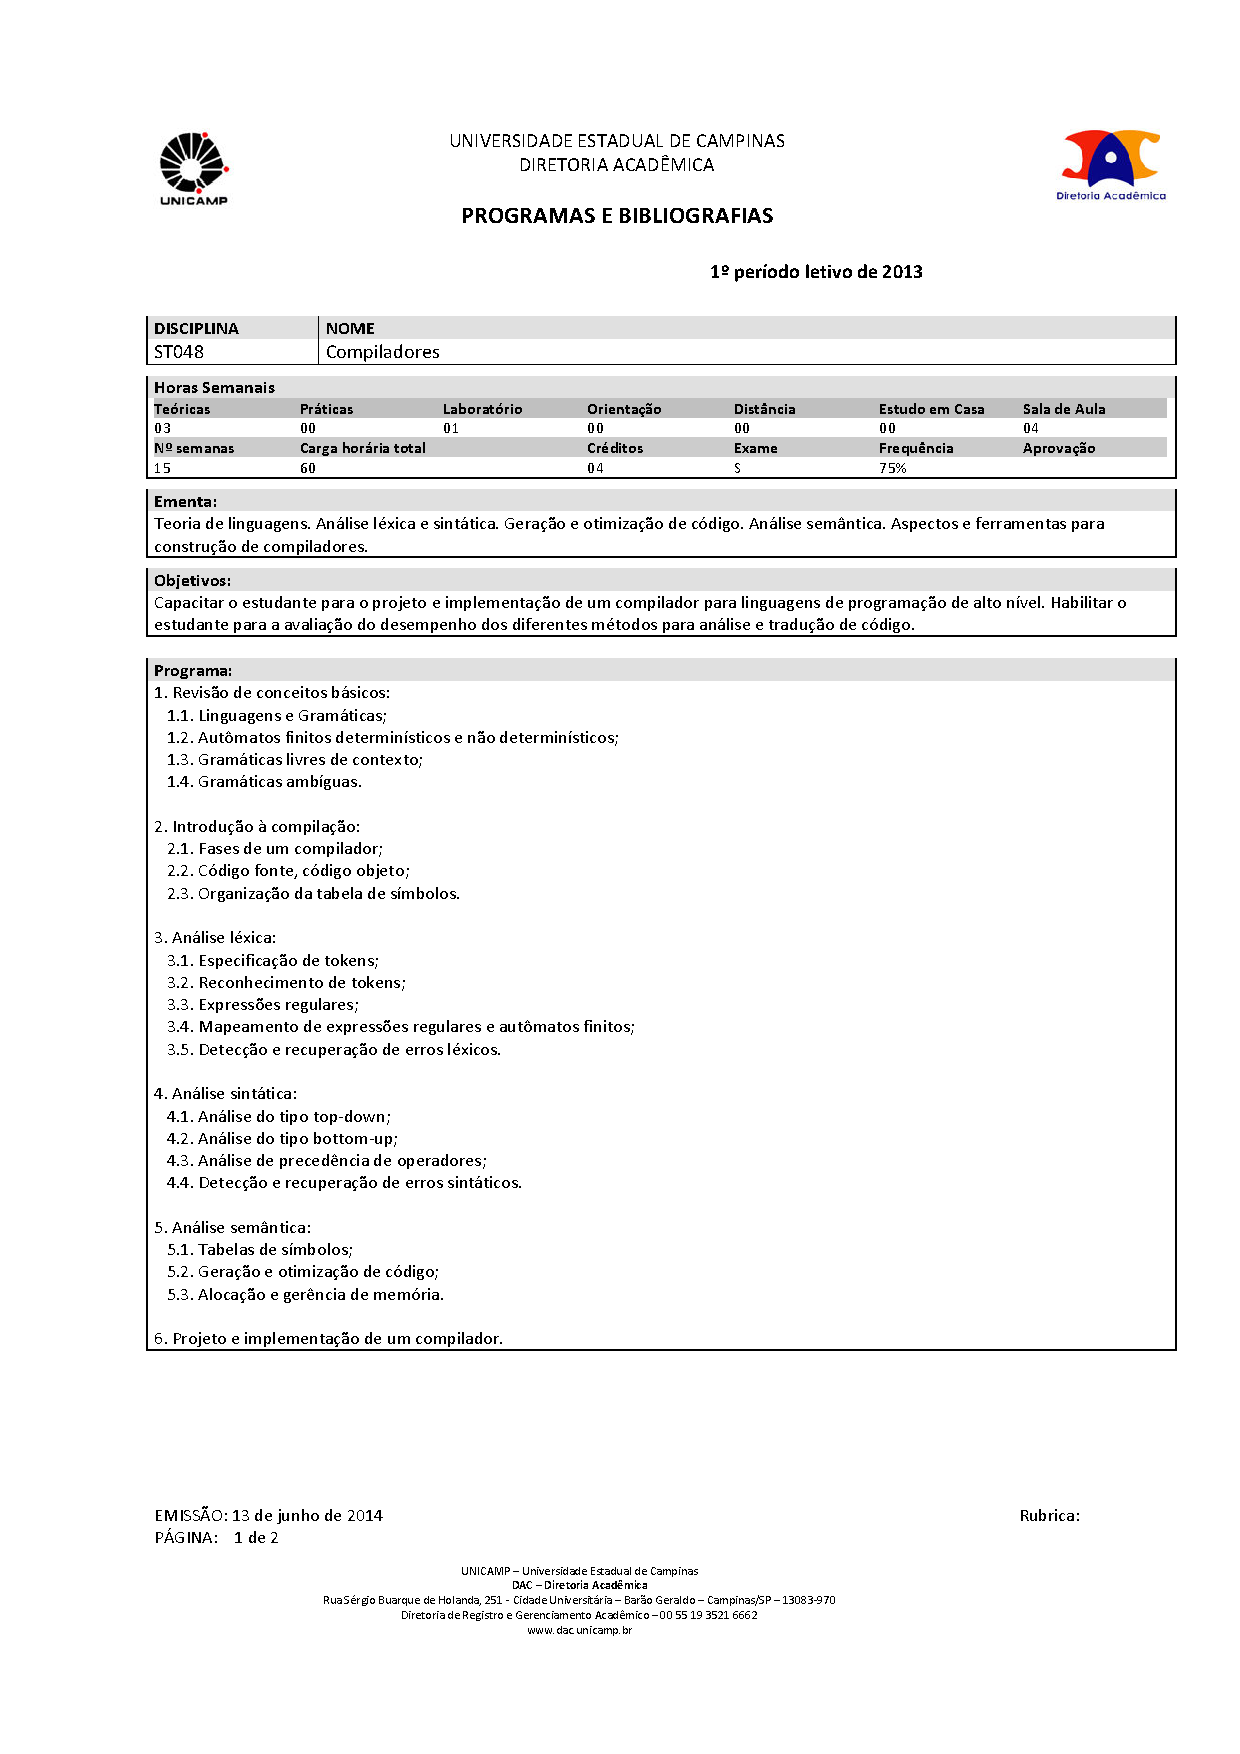
\includepdf{./docs/6_2_ProgramaDACCompiladores}
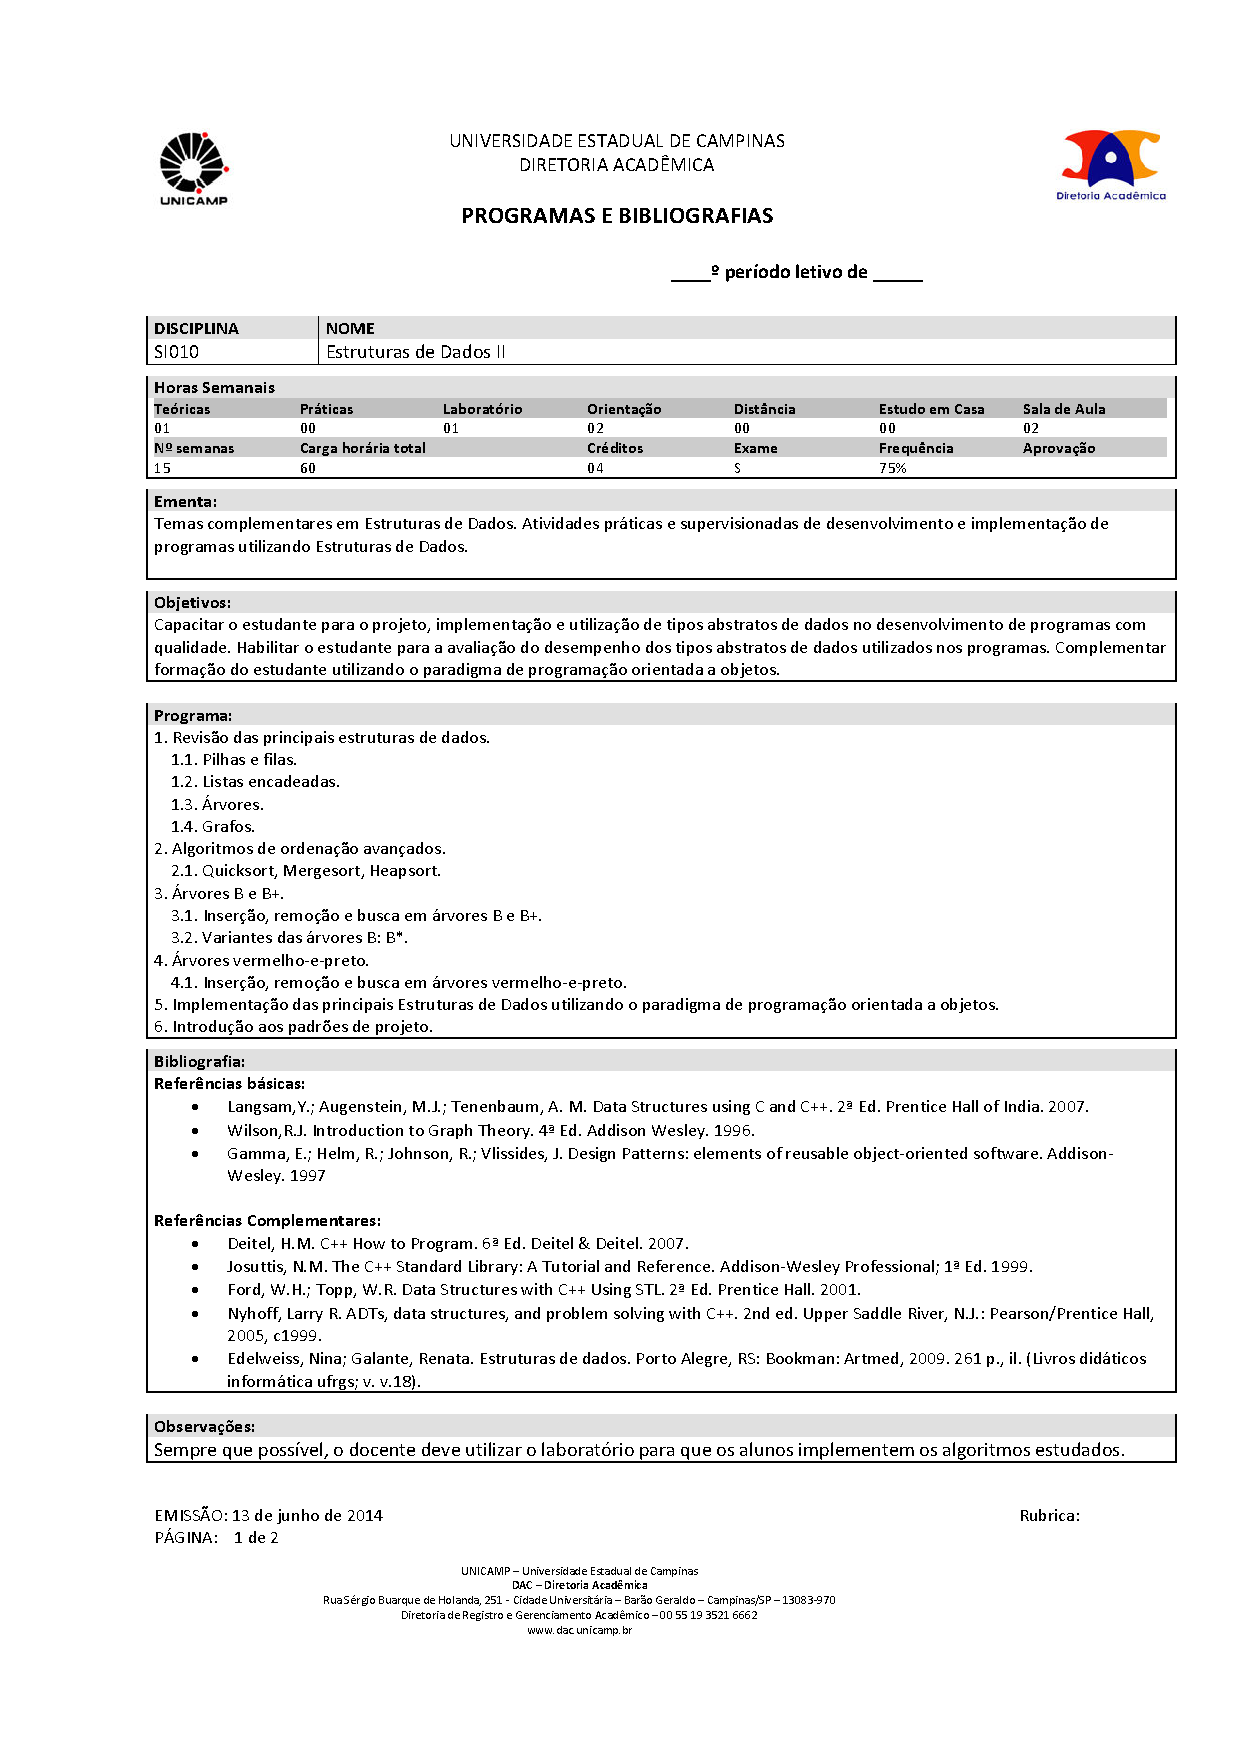
\includepdf{./docs/6_3_ProgramaDACEstruturasDadosII}
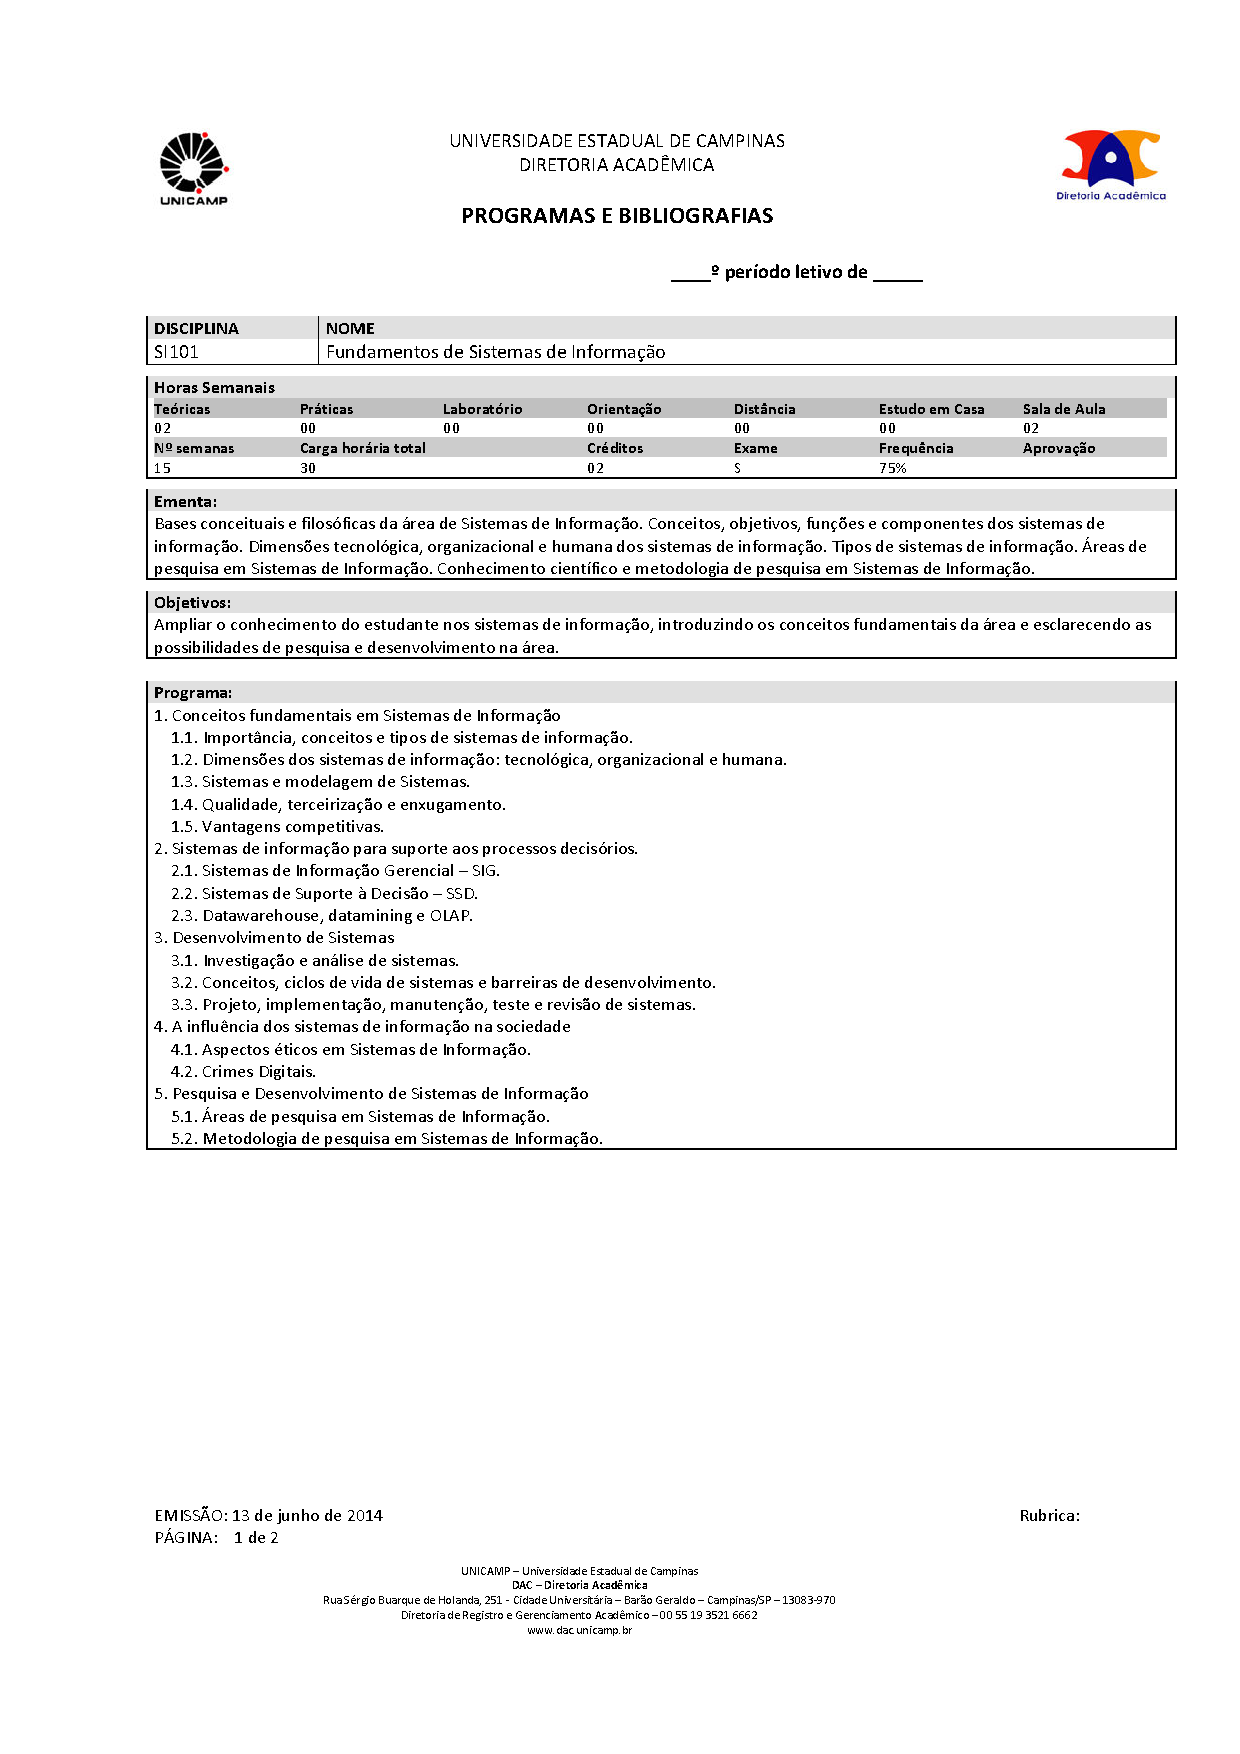
\includepdf{./docs/6_4_ProgramaDACFundamentosSistemasInformacao}
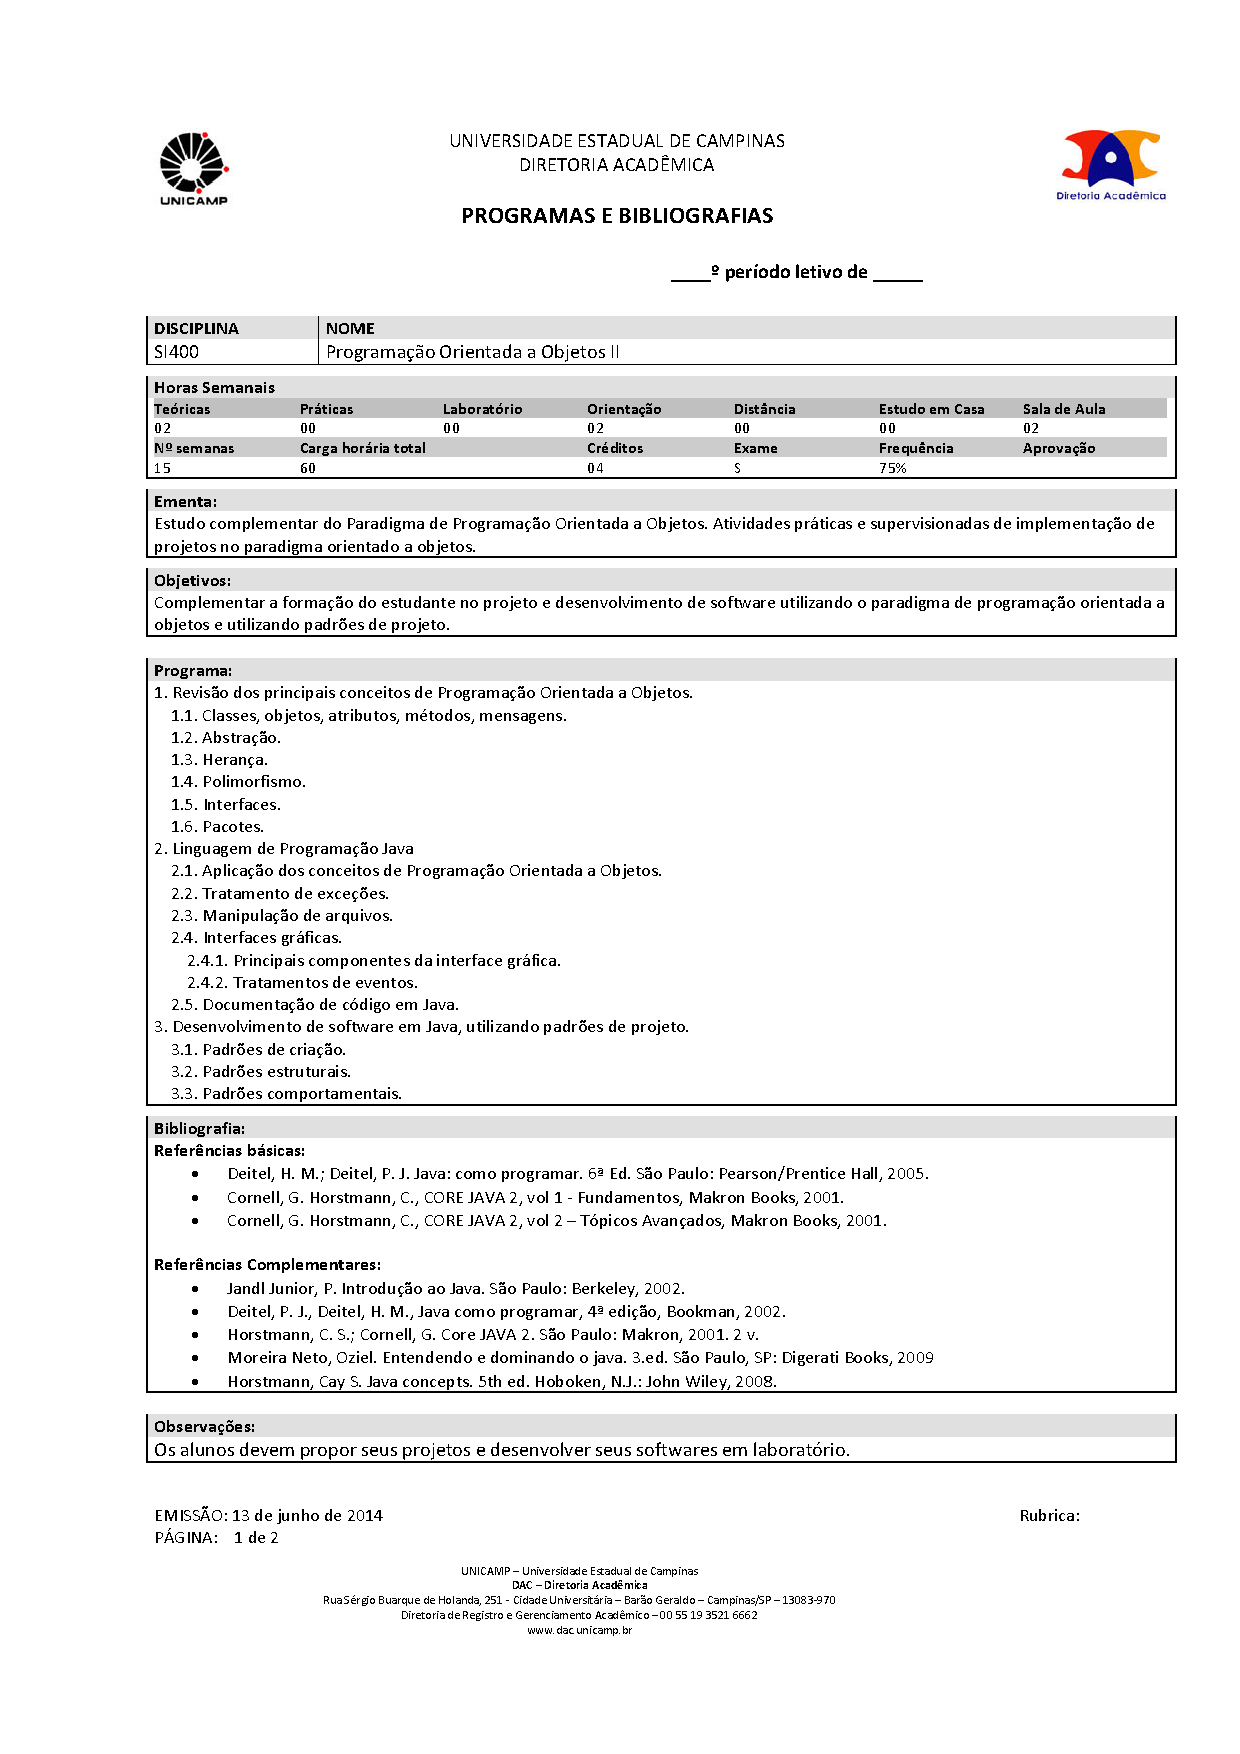
\includepdf{./docs/6_5_ProgramaDACProgramacaoOrientadaObjetosII}
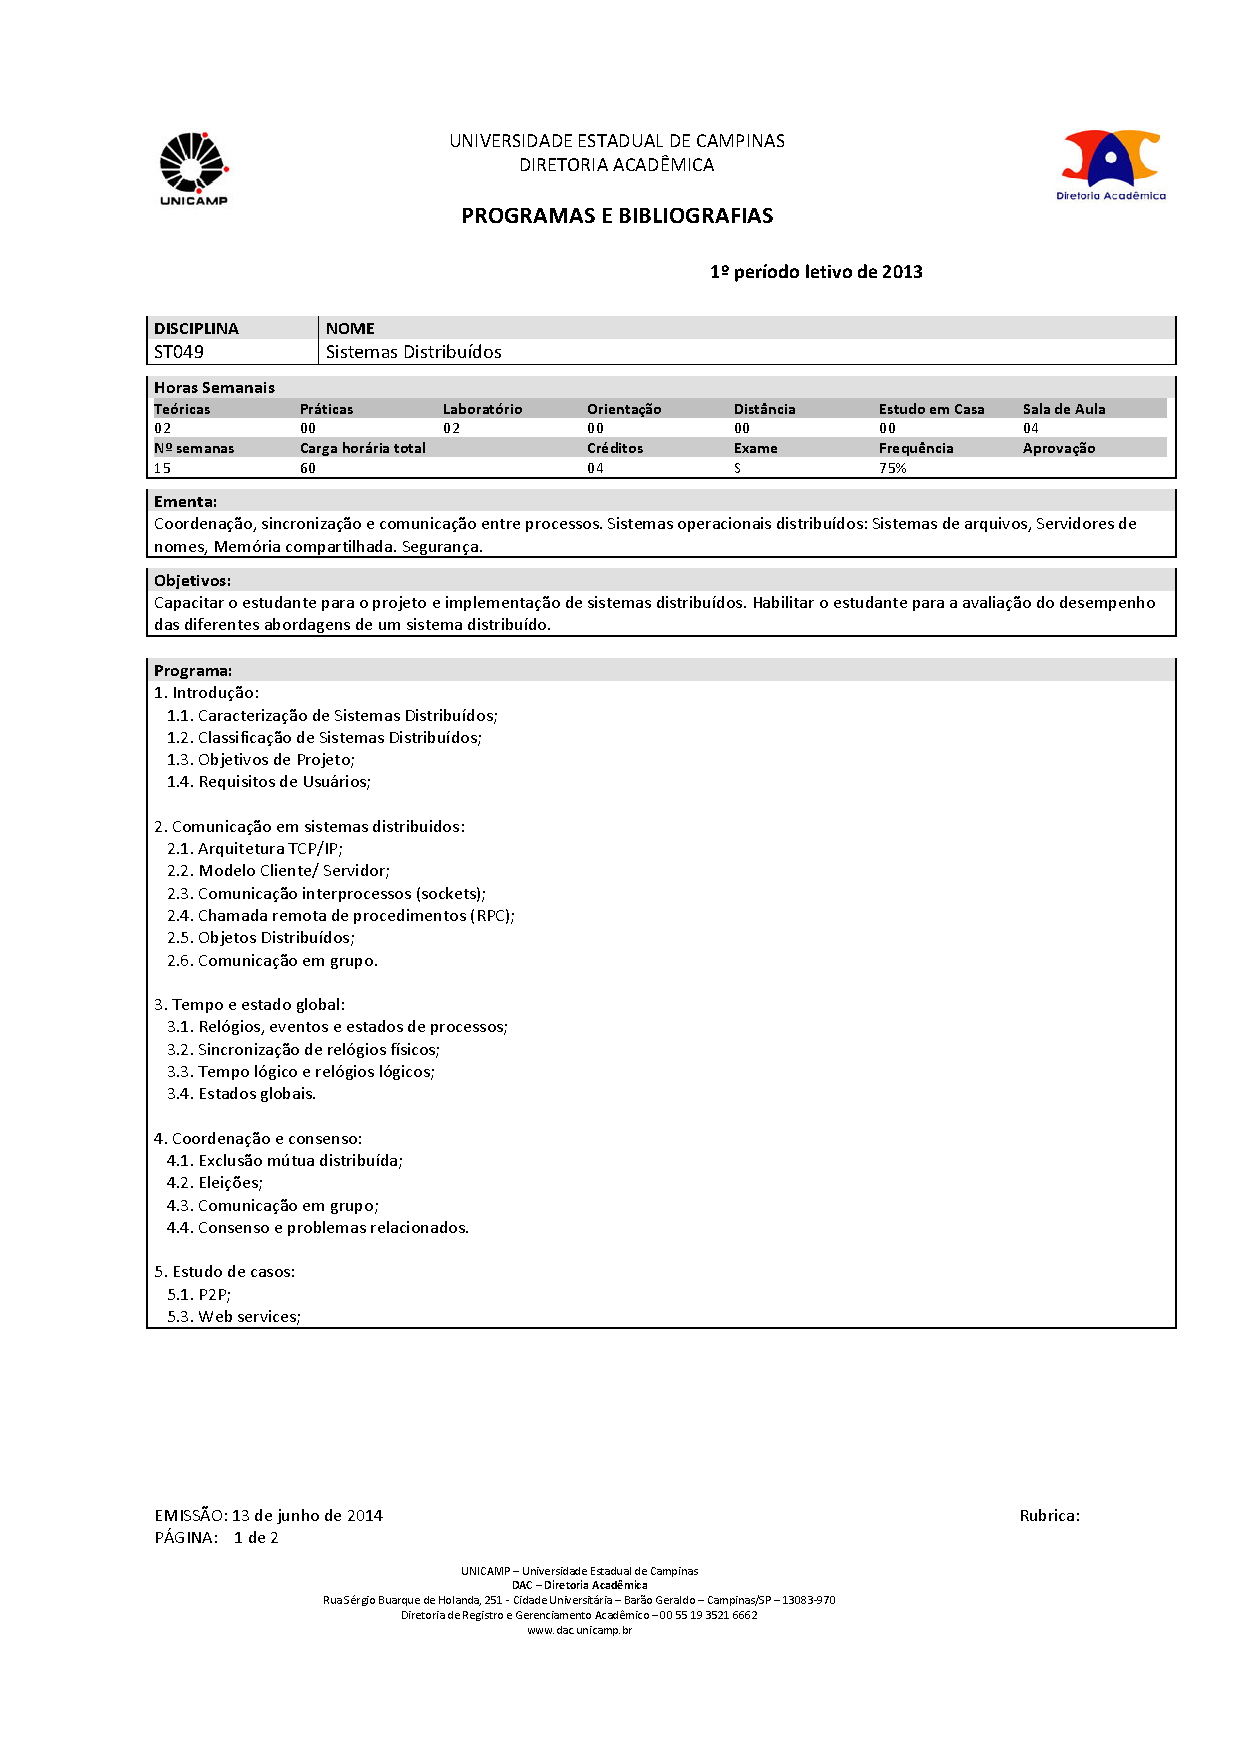
\includepdf{./docs/6_6_ProgramaDACSistemasDistribuidos}
%
%
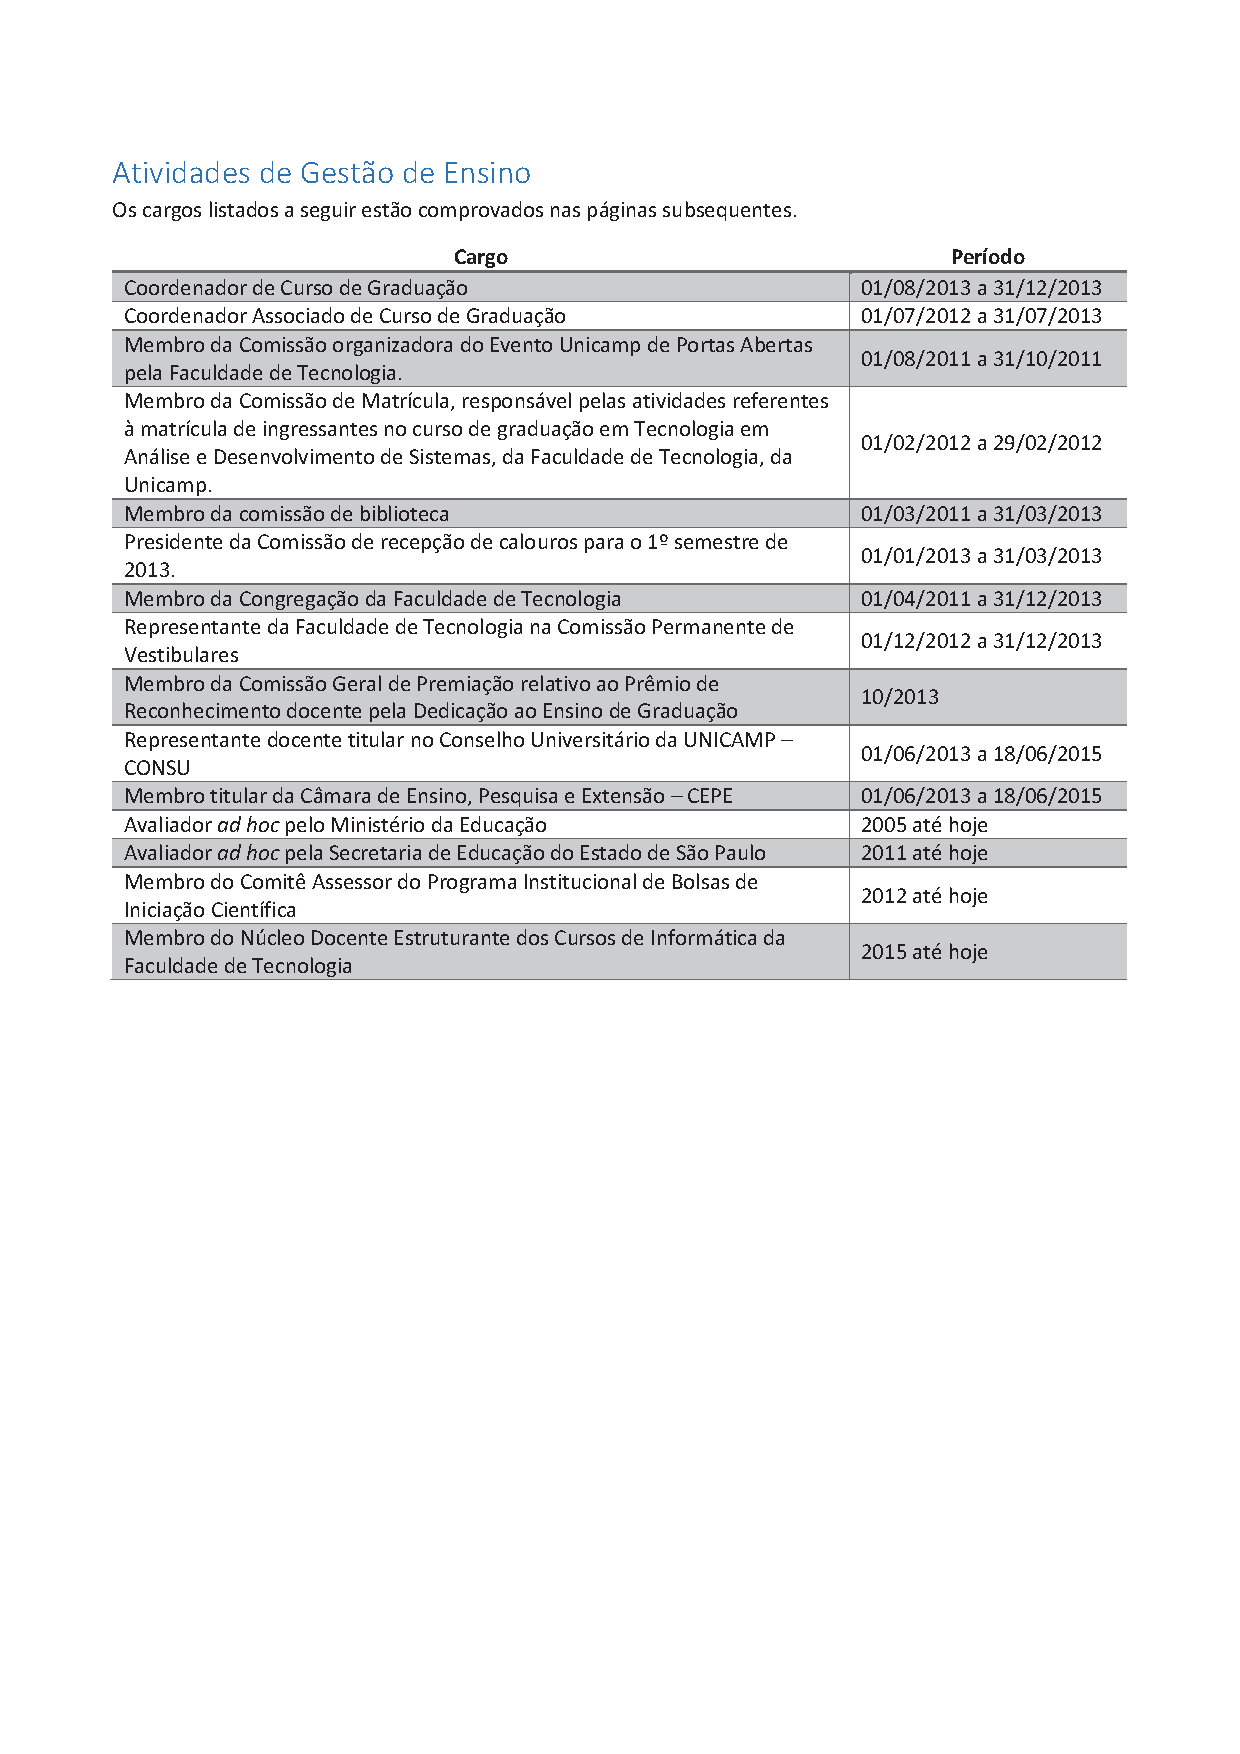
\includepdf{AtividadesGestao.pdf}
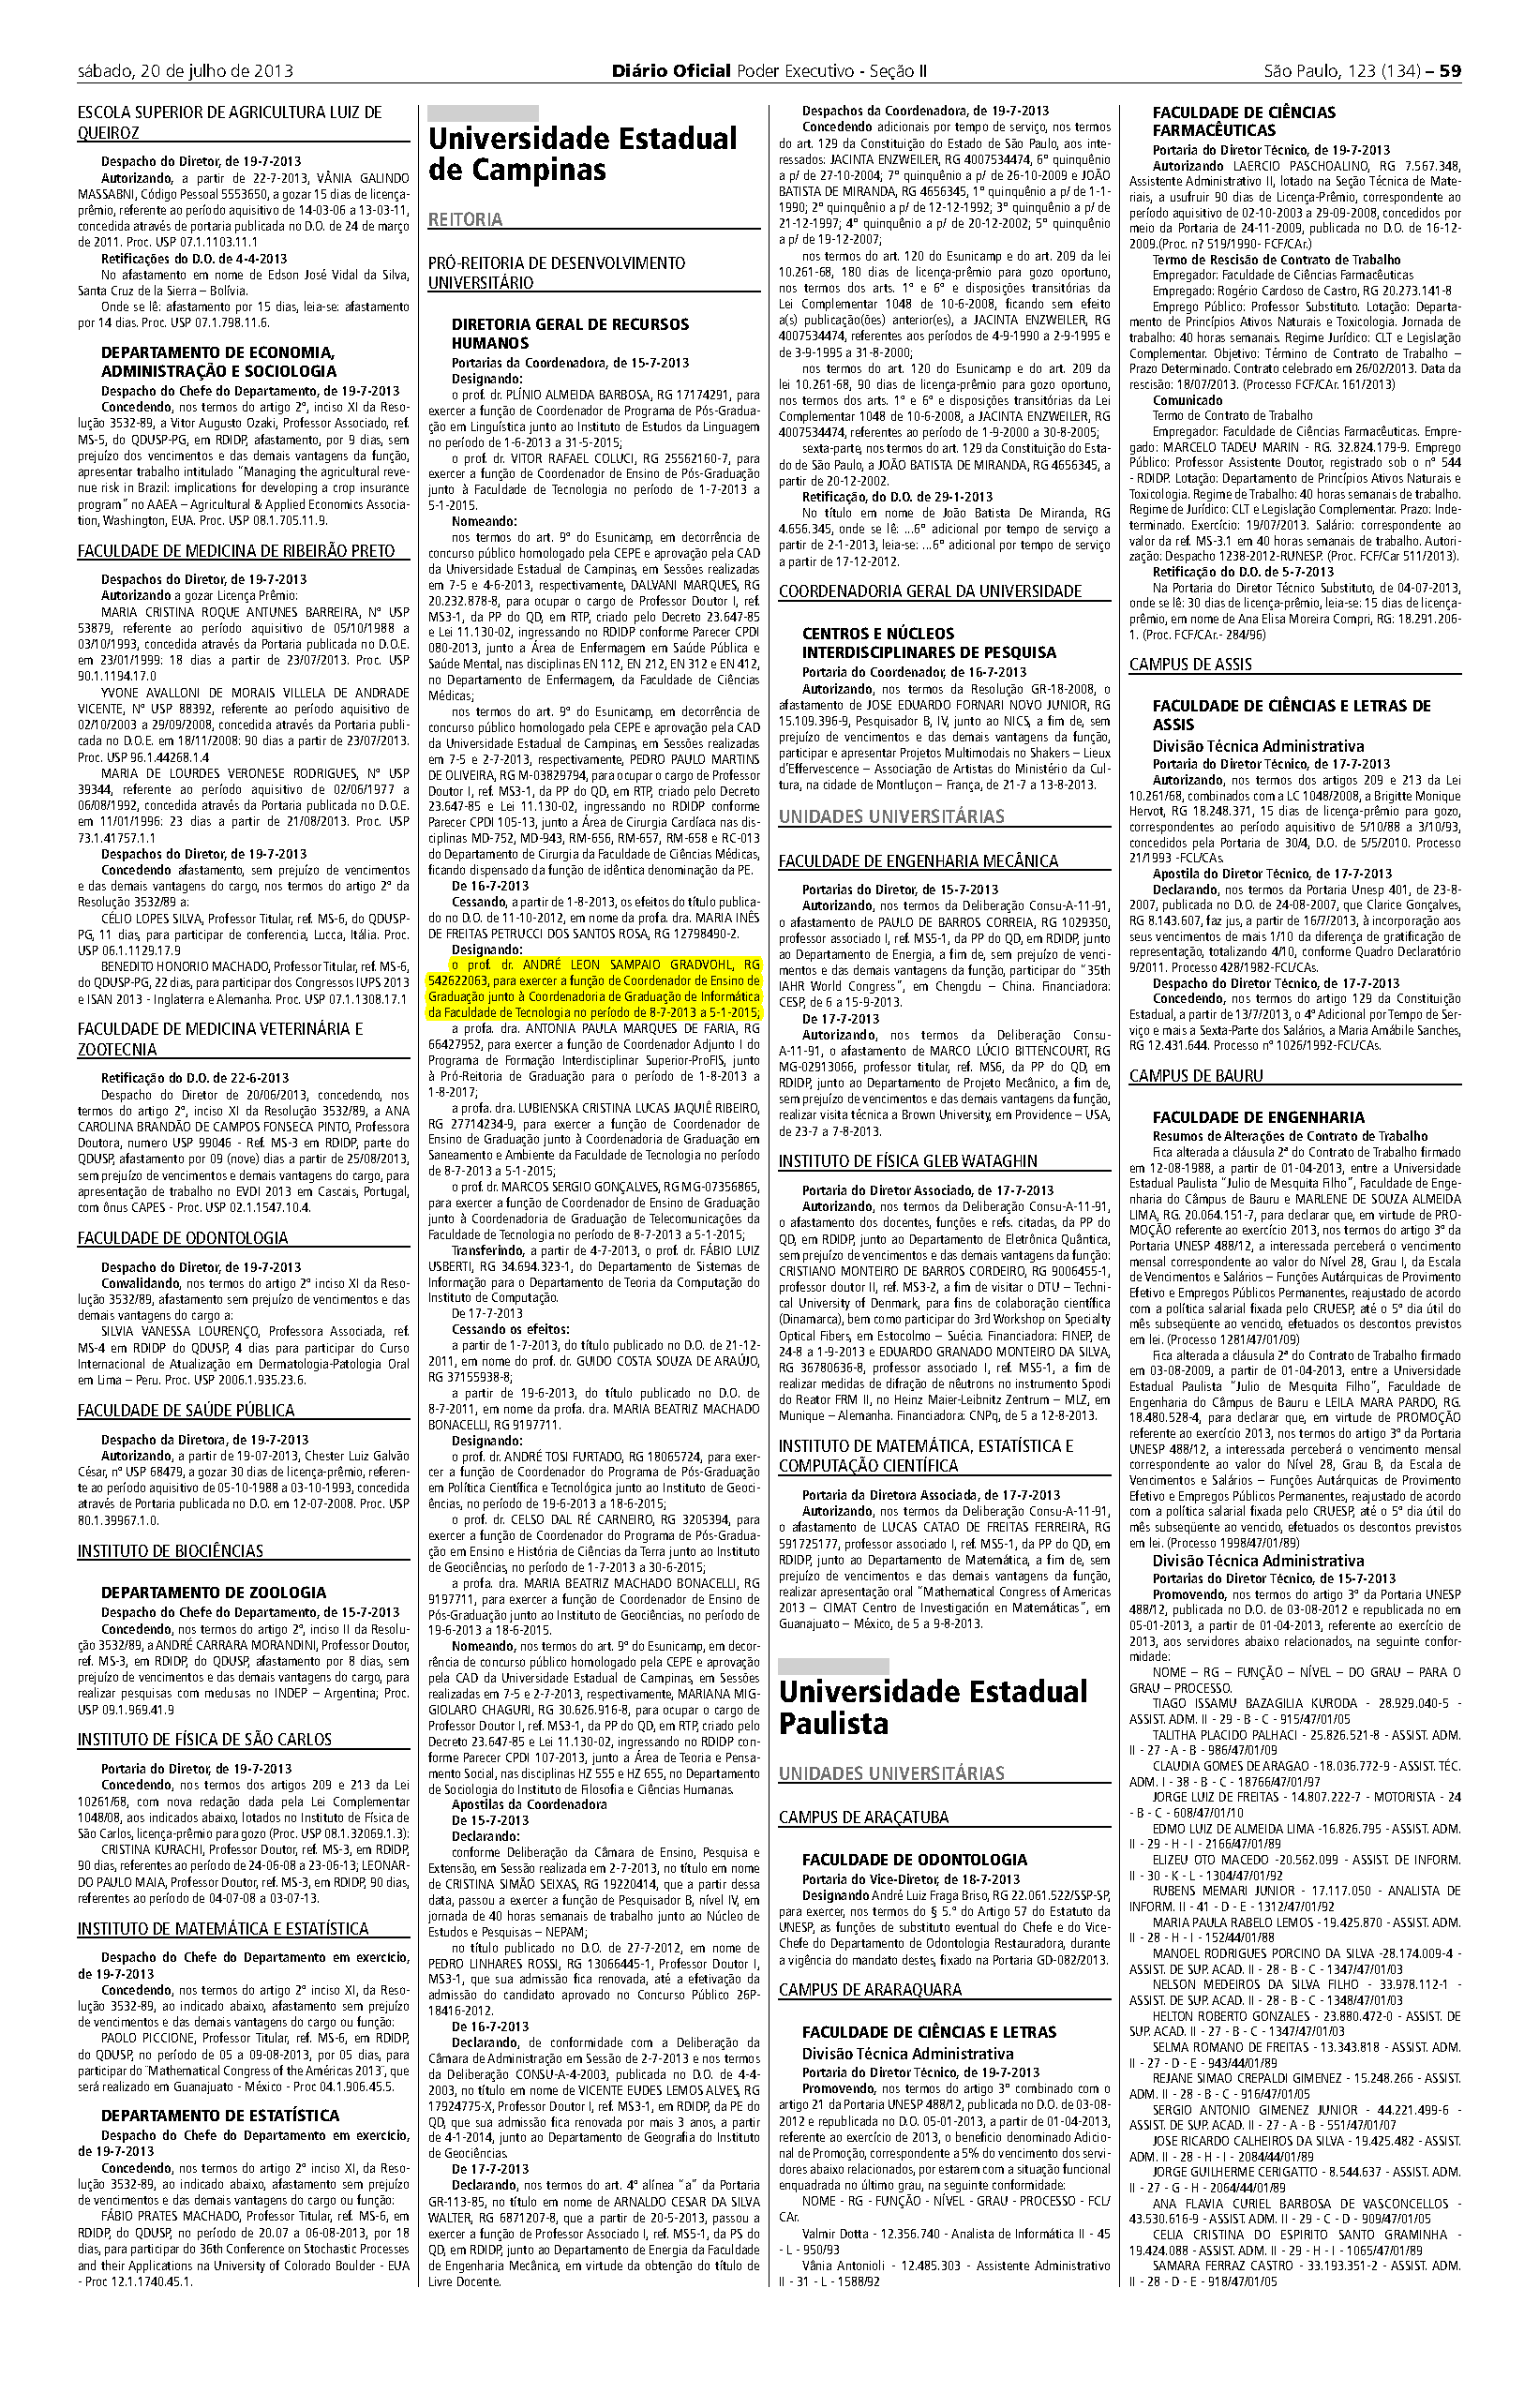
\includepdf{./docs/7_1_OficioDesignacaoCoordenadorInformaticaUnicamp}
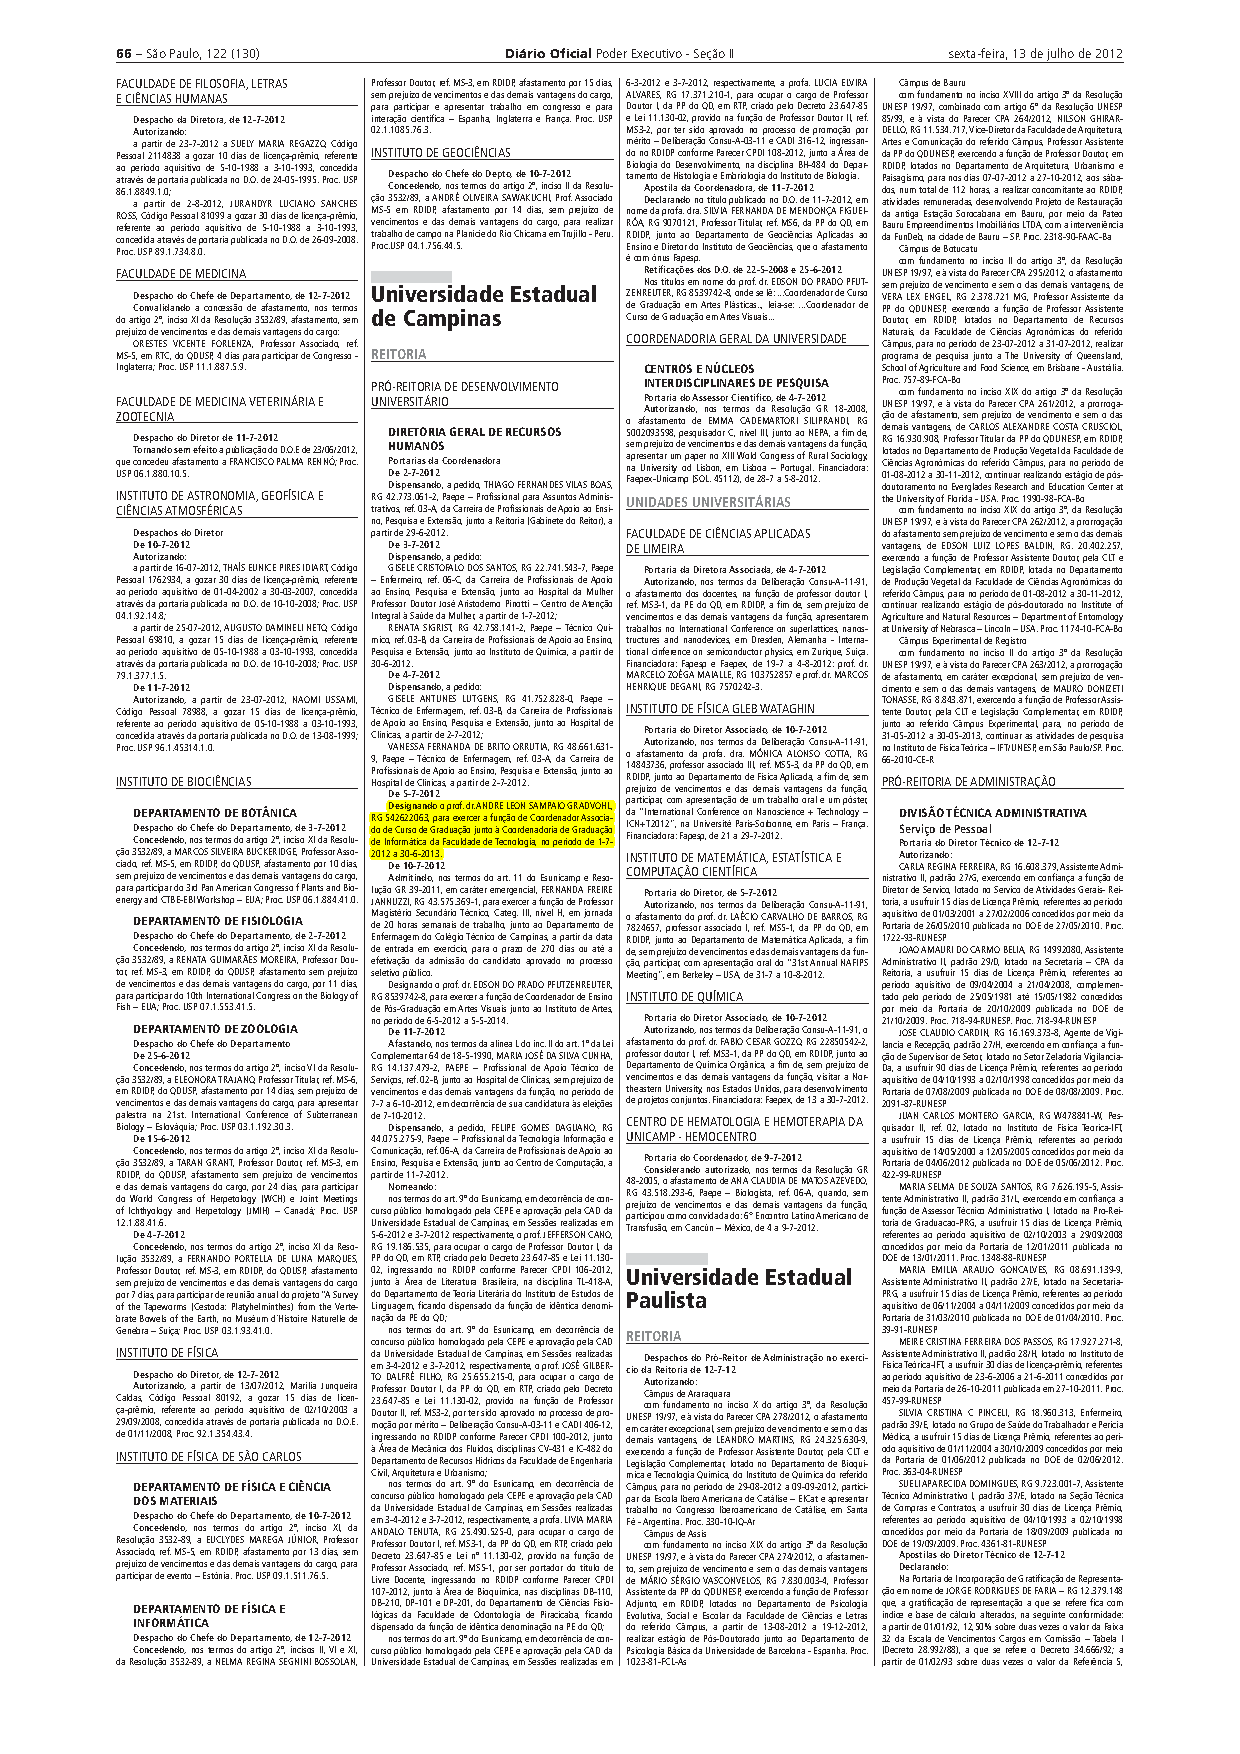
\includepdf{./docs/7_2_OficioDesignacaoCoordenadorAssociadoTADS}
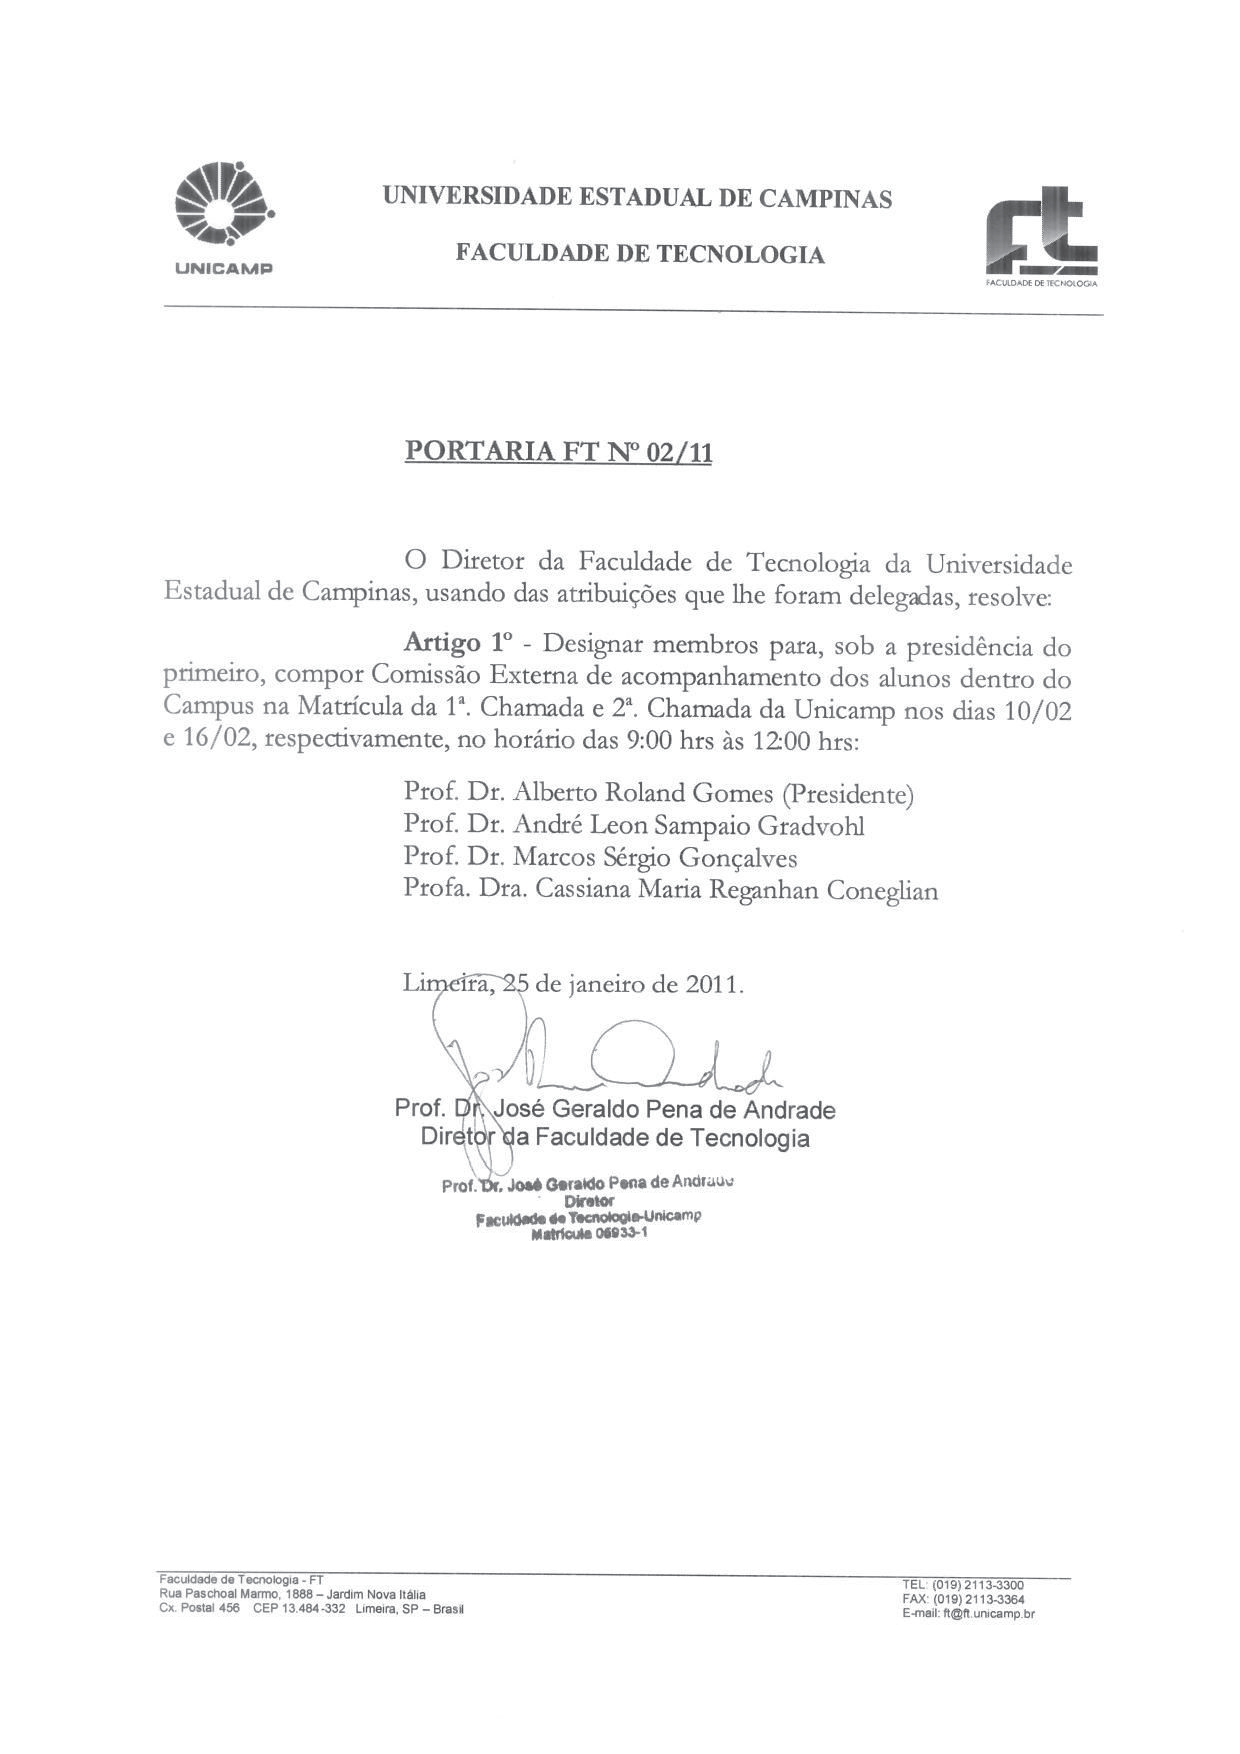
\includepdf{./docs/7_3_PortariaComisaoMatricula2012}
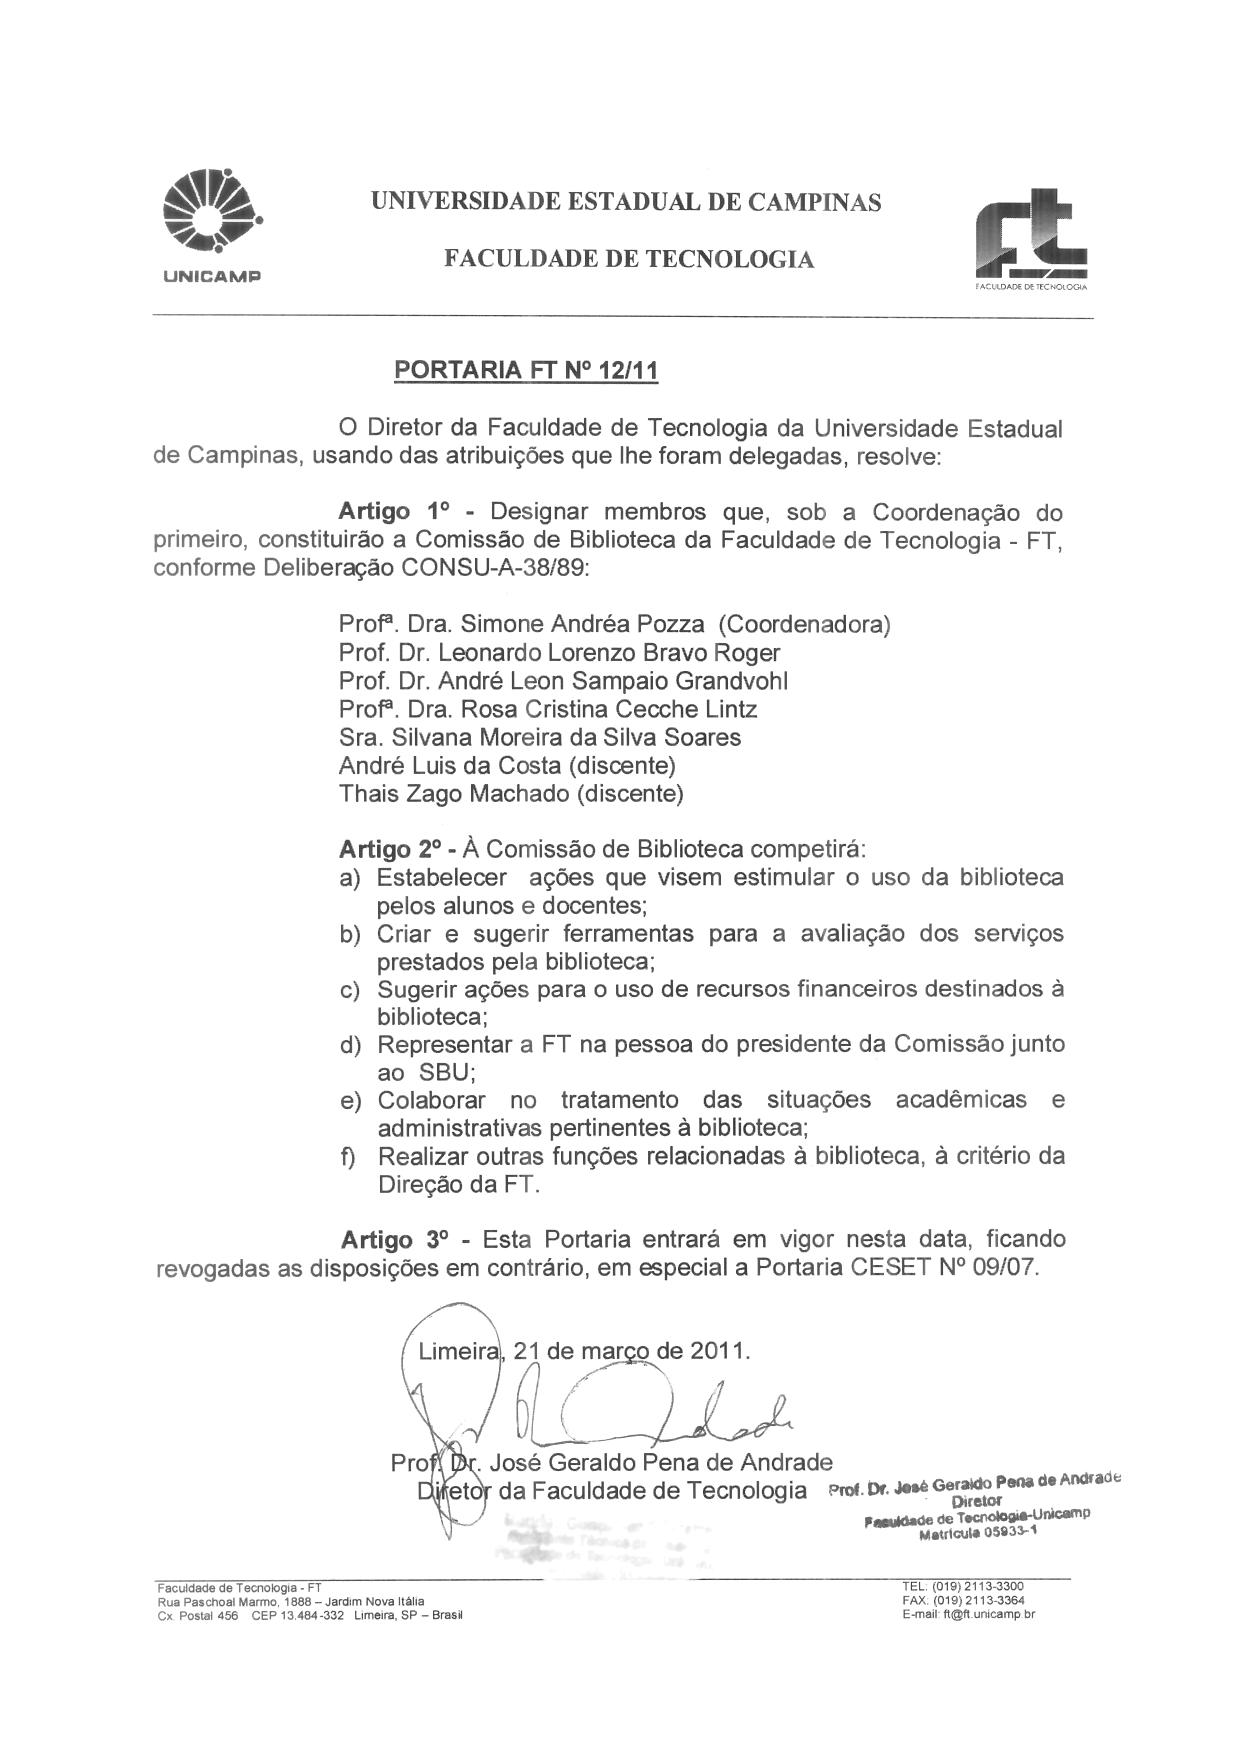
\includepdf{./docs/7_4_PortariaComissaoBiblioteca}
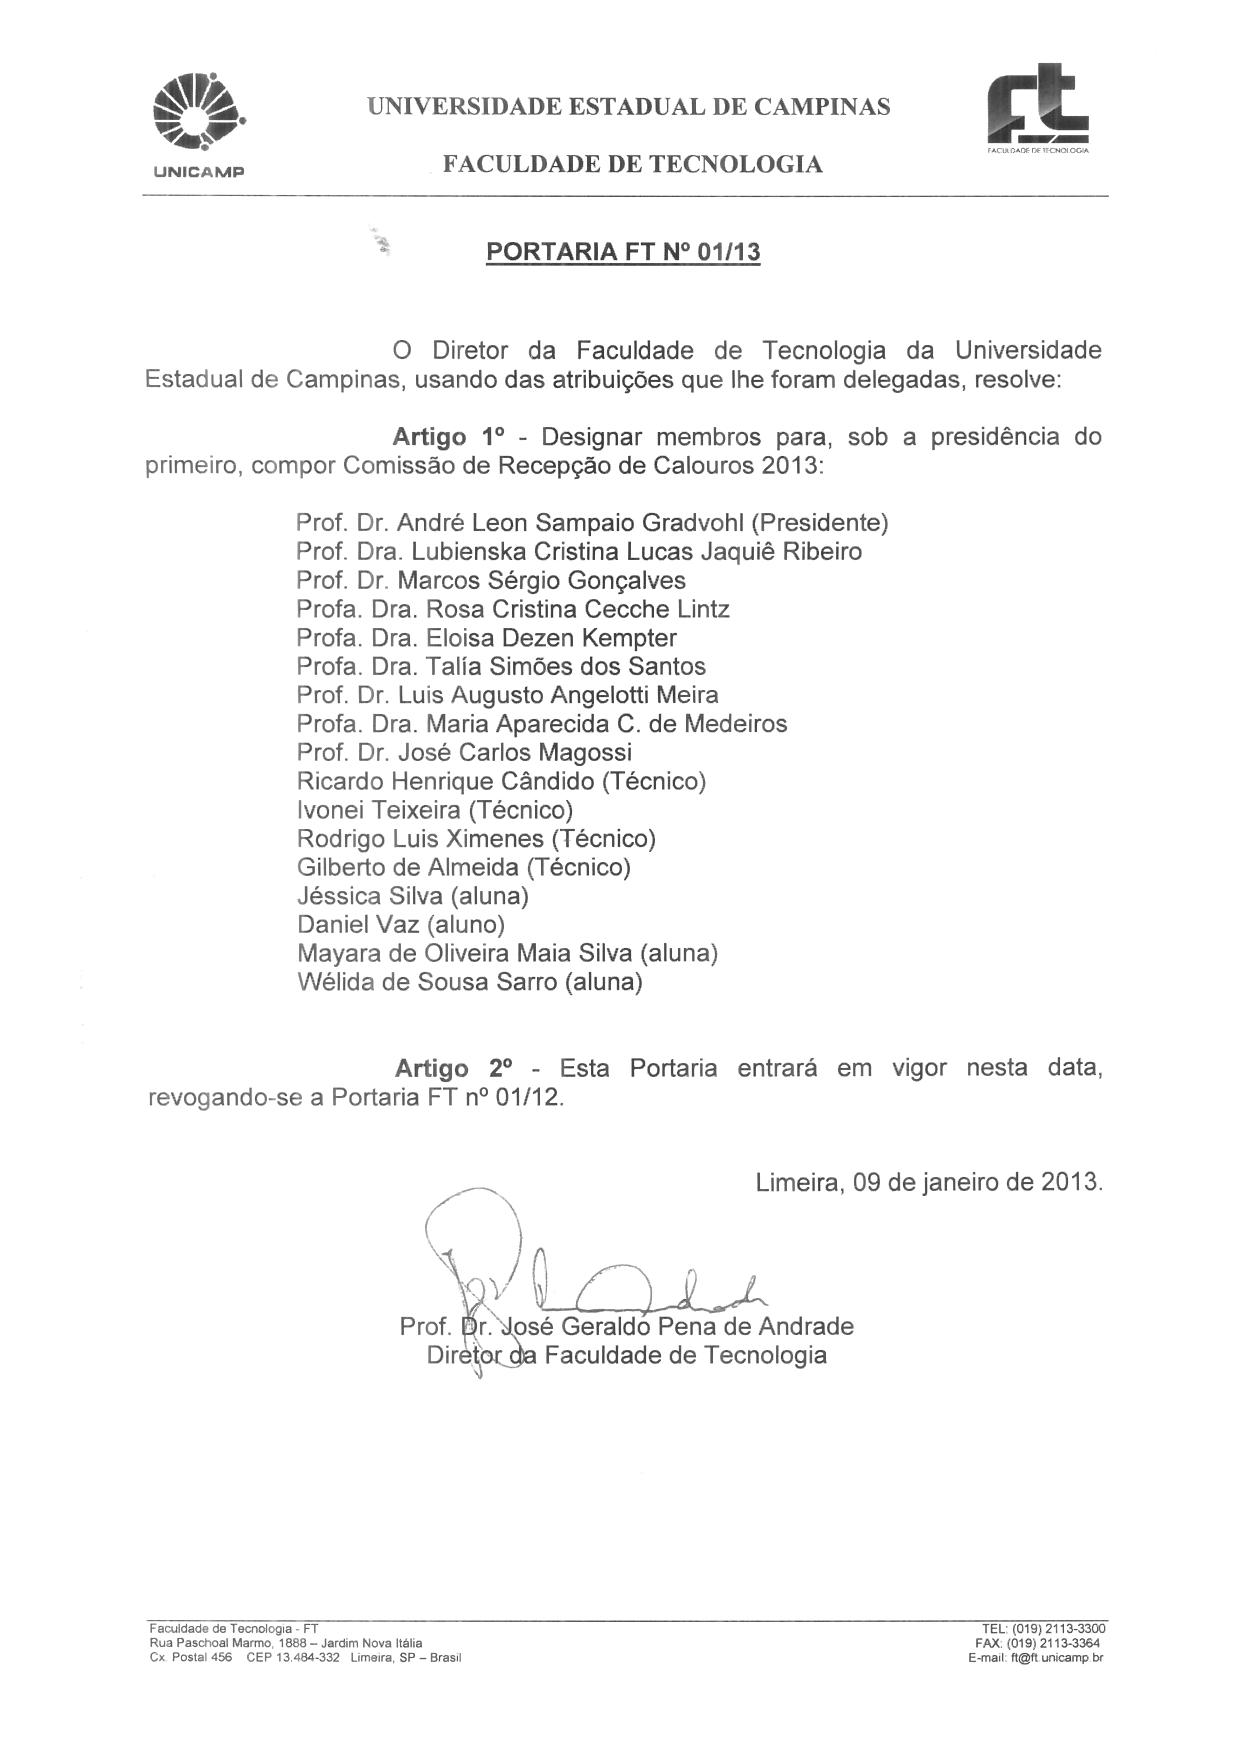
\includepdf{./docs/7_5_PresidenteComissaoRecepcaoCalouros2013}
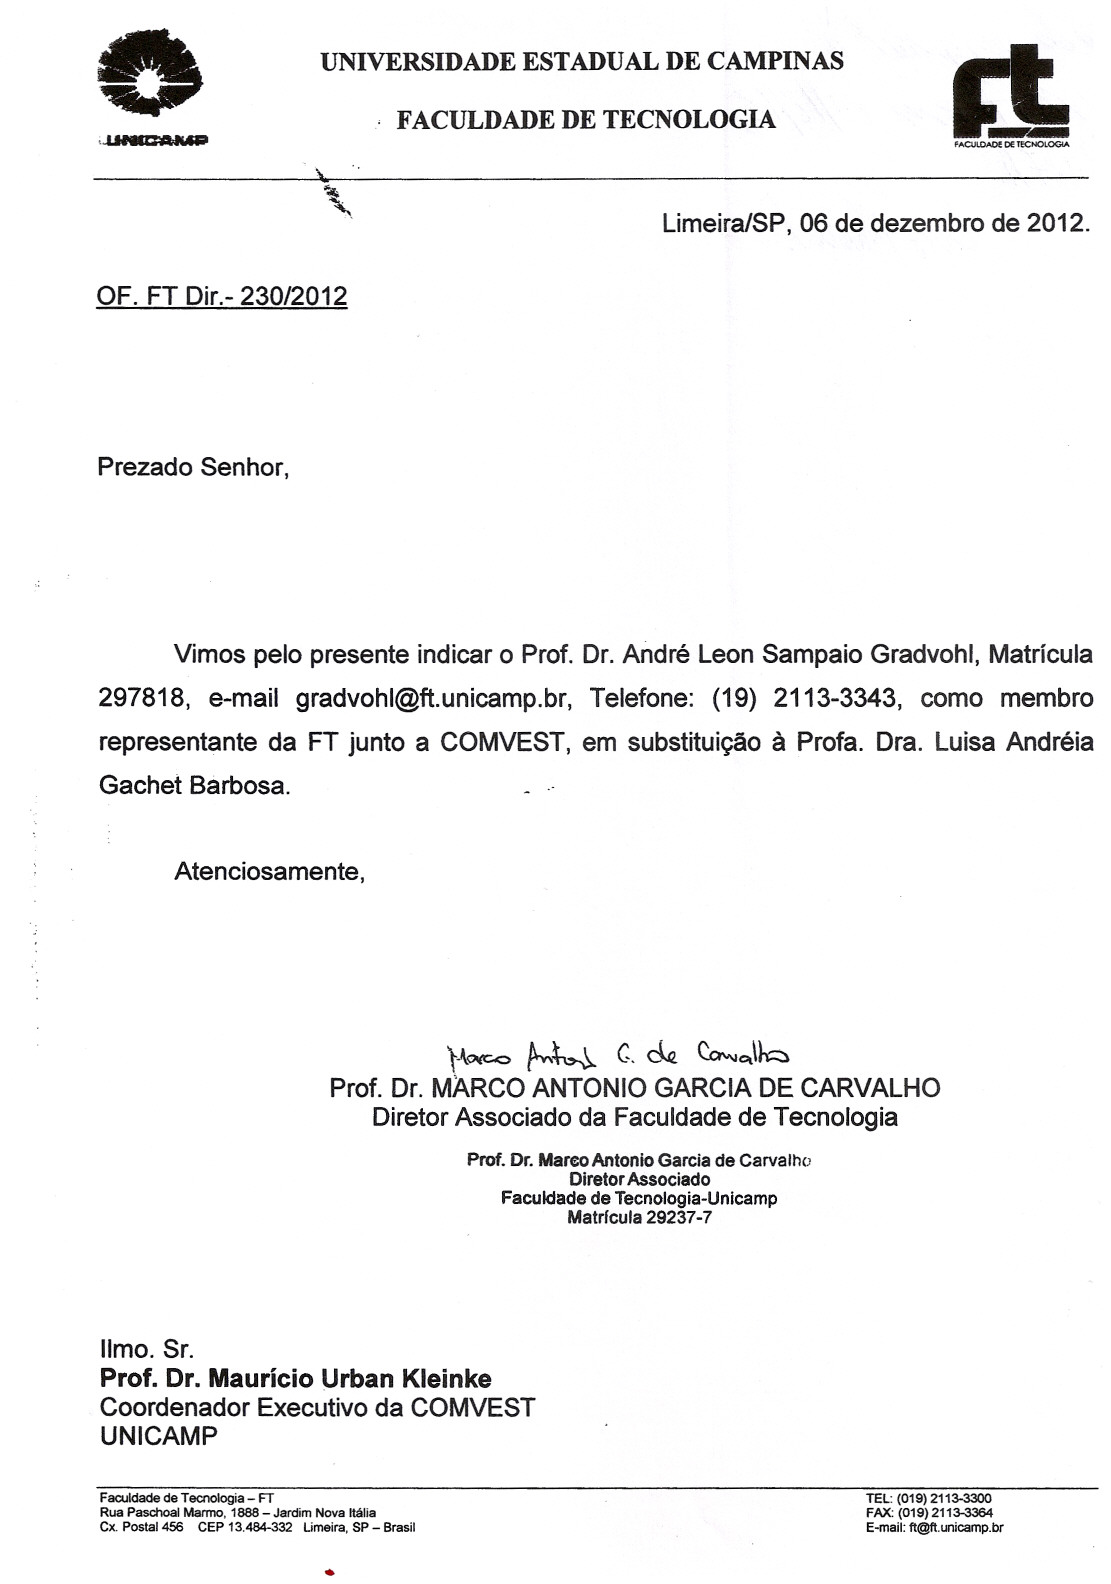
\includepdf{./docs/7_6_DeclaracaoParticipacaoComvest}
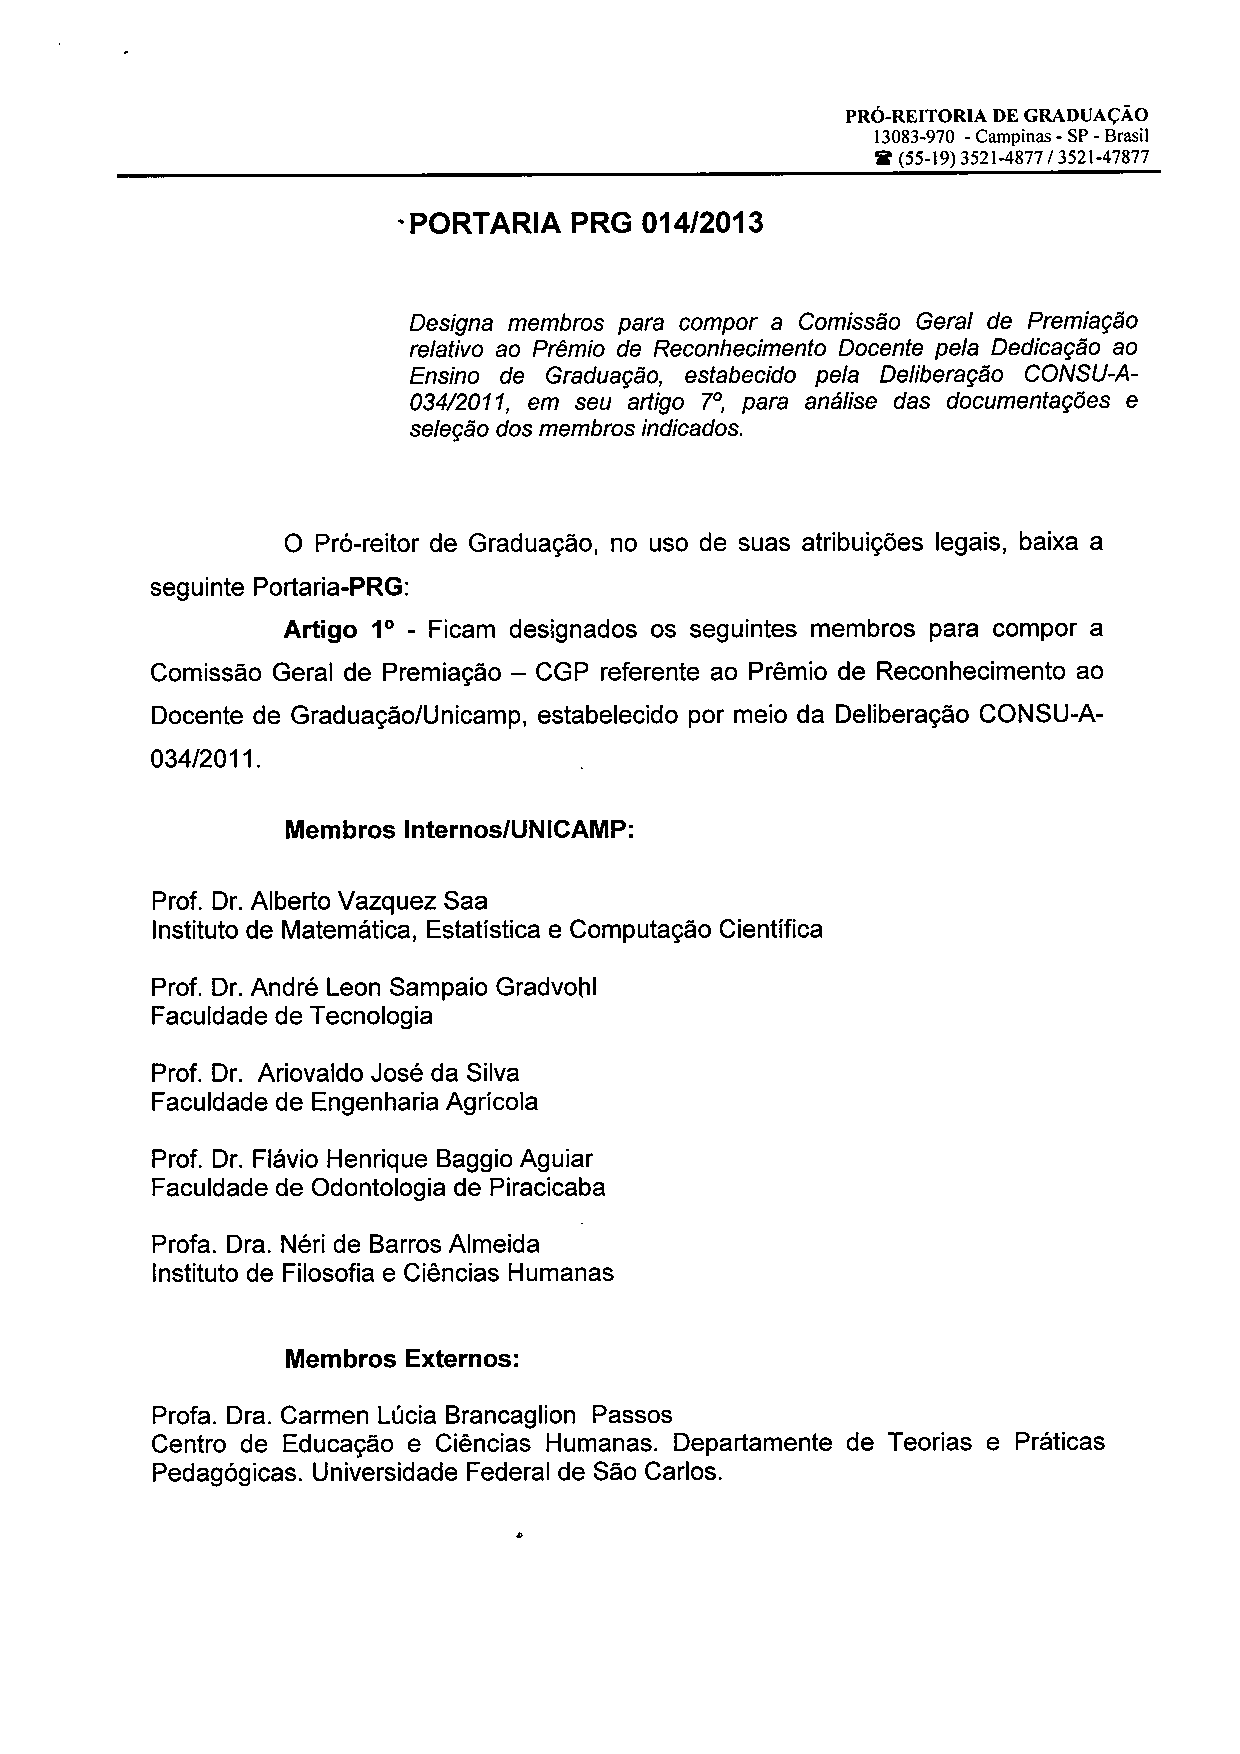
\includepdf{./docs/7_7_PortariaComissaoReconhecimentoDocente}
\includepdf{./docs/7_8_AtaEleicaoCONSU}
\includepdf{./docs/7_9_ParticipacaoCEPE}
\includepdf{./docs/7_10_ComprovanteAvaliacoesINEP}
\includepdf{./docs/7_11_ComprovanteAvaliacoesINEP_Atual}
\includepdf{./docs/7_12_DesignacaoAvaliadorCEESP_1}
\includepdf{./docs/7_13_DesignacaoAvaliadorCEESP_2}
\includepdf{./docs/7_14_DesignacaoAvaliadorCEESP_3}
\includepdf{./docs/7_15_DesignacaoAvaliadorCEESP_4}
\includepdf{./docs/7_16_DesignacaoAvaliadorCEESP_5}
\includepdf{./docs/7_17_PortariaComitePibic2012}
\includepdf{./docs/7_18_Portaria02_2013_ComitePibic}
\includepdf{./docs/7_19_Portaria042014_ComitePibic}
\includepdf{./docs/7_20_Portaria02_2015_ComitePibic}
\includepdf{./docs/7_21_Portaria04_2016_ComitePibic}
\includepdf{./docs/7_22_Portaria_NDE}
%
%
\includepdf{Intercambio.pdf}
\includepdf{./docs/8_1_ParticipacaoTopEspanha}
%
%
\includepdf{NovasMetodologias.pdf}
\includepdf{./docs/9_1_FormularioSTS}
%
%
\includepdf{Honrarias.pdf}
\includepdf{./docs/10_1_CertificateContestantHonorable_ACM_2012}
\includepdf{./docs/10_2_CertificateTeamHonorable_ACM_2012}
\includepdf{./docs/10_3_ConviteParaninfo_2014_2}
\includepdf{./docs/10_4_CertificadoParaninfo2015_2}
\includepdf{./docs/10_5_CertificadoParaninfo2016_1}

\includepdf{./docs/CertificadoParaninfo_2Sem2016}
\includepdf{./docs/CertificadoParaninfo_2Sem2017}
\includepdf{./docs/ConviteHomenageado2018}
\includepdf{./docs/certificadoParaninfo_2_2018}
\includepdf{./docs/10_6_CertificadoProfessorInovador2015}
\includepdf{./docs/10_7_CertificadoSeniorMemberIEEE}
\end{document}
